\documentclass[10pt]{article}
\usepackage{amsmath}
\usepackage{amssymb}
\usepackage{amsfonts}
\usepackage{amsthm}
\usepackage{amsbsy}
\usepackage{bm}
\usepackage[letterpaper, margin=1in]{geometry}
\usepackage[utf8]{inputenc}
\usepackage{appendix}
\usepackage{fancyhdr}
\usepackage{setspace}
\setlength{\parindent}{0pt}
\pagestyle{fancy}
\lhead{}
\rhead{}
\chead{}
\renewcommand{\headrulewidth}{0pt}
\usepackage{enumerate}
\usepackage{enumitem}
\renewcommand{\labelenumi}{\textbf{\arabic{enumi}.}}
\usepackage[normalem]{ulem}
\usepackage{graphicx}
\usepackage{float}
\usepackage{caption}
\usepackage{xspace}
\usepackage{xparse}
\usepackage[svgnames]{xcolor}
\usepackage[colorlinks, linkcolor=blue, anchorcolor=blue, urlcolor=red, citecolor=ForestGreen]{hyperref}
\usepackage[noabbrev, nameinlink, capitalise]{cleveref}
\usepackage{url}
\def\UrlBreaks{\do\A\do\B\do\C\do\D\do\E\do\F\do\G\do\H\do\I\do\J\do\K\do\L\do\M\do\N\do\O\do\P\do\Q\do\R\do\S\do\T\do\U\do\V\do\W\do\X\do\Y\do\Z\do\[\do\\\do\]\do\^\do\_\do\`\do\a\do\b\do\c\do\d\do\e\do\f\do\g\do\h\do\i\do\j\do\k\do\l\do\m\do\n\do\o\do\p\do\q\do\r\do\s\do\t\do\u\do\v\do\w\do\x\do\y\do\z\do\.\do\@\do\\\do\/\do\!\do\_\do\|\do\;\do\>\do\]\do\)\do\,\do\?\do\'\do+\do\=\do\#}
\usepackage{natbib}
\bibliographystyle{abbrvnat}
\setcitestyle{authoryear,open={(},close={)}}
\usepackage{tikz}

\crefname{section}{Sec.}{Secs.}
\crefname{appendix}{App.}{Apps.}
\crefname{table}{Tab.}{Tabs.}
\crefname{figure}{Fig.}{Figs.}
\crefname{equation}{Eq.}{Eqs.}

\theoremstyle{plain}
\newtheorem{theorem}{Theorem}
\crefname{theorem}{Thm.}{Thms.}
\newtheorem{lemma}[theorem]{Lemma}
\crefname{lemma}{Lem.}{Lems.}
\newtheorem{assumption}{Assumption}
\crefname{assumption}{Assump.}{Assumps.}
\newtheorem{proposition}[theorem]{Proposition}
\crefname{proposition}{Prop.}{Props.}
\newtheorem{corollary}[theorem]{Corollary}
\crefname{corollary}{Cor.}{Cors.}
\newtheorem{definition}[theorem]{Definition}
\crefname{definition}{Def.}{Defs.}
\newtheorem{remark}[theorem]{Remark}
\crefname{remark}{Rmk.}{Rmks.}
\newenvironment{sketchofproof}{\paragraph{\textbf{Sketch of Proof}}}{\hfill$\square$}
\usepackage[ruled, vlined, linesnumbered, commentsnumbered]{algorithm2e}
\crefname{algocf}{Alg.}{Algs.}

\usepackage{newtxtext}
\newcommand{\ro}[1]{\left(#1\right)}
\newcommand{\sq}[1]{\left[#1\right]}
\newcommand{\sqd}[1]{\left[\!\left[#1\right]\!\right]}
\newcommand{\cu}[1]{\left\{#1\right\}}
\newcommand{\abs}[1]{\left|#1\right|}
\newcommand{\norm}[1]{\left\|#1\right\|}
\newcommand{\inn}[1]{\left\langle#1\right\rangle}
\newcommand{\ceil}[1]{\left\lceil#1\right\rceil}
\newcommand{\floor}[1]{\left\lfloor#1\right\rfloor}

\newcommand{\e}{\mathrm{e}}

\newcommand{\pif}{{+\infty}}
\newcommand{\nif}{{-\infty}}

\newcommand{\tp}{^\mathrm{T}}

\newcommand{\const}{\operatorname{const}}
\newcommand{\id}{\operatorname{id}}

\renewcommand{\P}{\mathbb{P}}
\newcommand{\E}{\operatorname{\mathbb{E}}}
\newcommand{\var}{\operatorname{Var}}
\newcommand{\bias}{\operatorname{Bias}}
\newcommand{\cov}{\operatorname{Cov}}
\newcommand{\corr}{\operatorname{Corr}}

\newcommand{\iid}{\stackrel{\mathrm{i.i.d.}}{\sim}}
\newcommand{\idd}{\stackrel{\mathrm{d}}{=}}
\newcommand{\aseq}{\stackrel{\mathrm{a.s.}}{=}}

\newcommand{\R}{\mathbb{R}}
\newcommand{\N}{\mathbb{N}}
\newcommand{\Z}{\mathbb{Z}}

\newcommand{\n}[1]{\operatorname{\mathcal{N}}\left(#1\right)}
\newcommand{\un}{\operatorname{Unif}}

\renewcommand{\d}{\mathrm{d}}
\newcommand{\de}[2]{\frac{\mathrm{d}#1}{\mathrm{d}#2}}
\newcommand{\pd}[2]{\frac{\partial#1}{\partial#2}}

\newcommand{\tr}{\operatorname{tr}}
\newcommand{\diag}{\operatorname{diag}}
\newcommand{\dist}[1]{\operatorname{dist}\left(#1\right)}

\newcommand{\argmin}{\mathop\mathrm{argmin}}
\newcommand{\argmax}{\mathop\mathrm{argmax}}

\newcommand{\kl}{\operatorname{KL}}
\newcommand{\tv}{\operatorname{TV}}
\newcommand{\fisher}{\operatorname{FI}}
\newcommand{\renyi}{\operatorname{R}}

\newcommand{\red}[1]{{\color{red}#1}}
\newcommand{\blue}[1]{{\color{blue}#1}}
\newcommand{\magenta}[1]{{\color{magenta}#1}}
\newcommand{\gray}[1]{{\color{gray}#1}}
\newcommand{\orange}[1]{{\color{orange}#1}}
\newcommand{\green}[1]{{\color{green}#1}}

\newcommand{\Ot}{\widetilde{O}}
\newcommand{\Thetat}{\widetilde{\Theta}}
\newcommand{\Omegat}{\widetilde{\Omega}}
\newcommand{\poly}{\operatorname{poly}}

\newcommand{\cA}{\mathcal{A}}
\newcommand{\cE}{\mathcal{E}}
\newcommand{\cF}{\mathcal{F}}
\newcommand{\cL}{\mathcal{L}}
\newcommand{\cW}{\mathcal{W}}
\newcommand{\prob}{\operatorname{Pr}}
\renewcommand{\Pr}{\mathbb{P}^\to}
\newcommand{\Pl}{\mathbb{P}^\gets}
\newcommand{\Qr}{\mathbb{Q}^\to}
\newcommand{\Ql}{\mathbb{Q}^\gets}
\newcommand{\Qd}{\mathbb{Q}^\dagger}
\newcommand{\Phr}{\widehat{\mathbb{P}}^\to}
\newcommand{\Ptr}{\widetilde{\mathbb{P}}^\to}
\newcommand{\Pbr}{\overline{\mathbb{P}}^\to}
\newcommand{\cPr}{\mathcal{P}^\to}
\newcommand{\cPl}{\mathcal{P}^\gets}
\newcommand{\cQ}{\mathcal{Q}}

\newcommand{\Q}{\mathbb{Q}}
\newcommand{\W}{\mathbb{W}}
\newcommand{\Pbf}{\mathbf{P}}
\newcommand{\Qh}{\widehat{\mathbb{Q}}}
\newcommand{\Qbf}{\mathbf{Q}}
\newcommand{\Qhbf}{{\mathbf{\widehat{Q}}}}
\newcommand{\Fh}{\widehat{F}}
\newcommand{\Gh}{\widehat{G}}
\newcommand{\Gt}{\widetilde{G}}
\newcommand{\ut}{\widetilde{u}}
\newcommand{\mut}{\widetilde{\mu}}

\newcommand{\xb}{\overline{x}}
\newcommand{\Xh}{\widehat{X}}
\newcommand{\Xt}{\widetilde{X}}
\newcommand{\Xb}{\overline{X}}
\newcommand{\Zh}{\widehat{Z}}
\newcommand{\ph}{\widehat{p}}
\newcommand{\pt}{\widetilde{p}}
\newcommand{\pb}{\overline{p}}
\newcommand{\clsi}{C_\mathrm{LSI}}
\newcommand{\cpi}{C_\mathrm{PI}}
\newcommand{\Bl}{B^\gets}
\newcommand{\Xl}{X^\gets}
\newcommand{\Xr}{X^\to}
\newcommand{\xl}{x^\gets}
\newcommand{\Yl}{Y^\gets}
\newcommand{\Zl}{Z^\gets}
\newcommand{\Ml}{M^\gets}
\newcommand{\rhoh}{\widehat{\rho}}
\newcommand{\rhob}{\overline{\rho}}
\newcommand{\rhot}{\widetilde{\rho}}
\newcommand{\al}{a^\gets}
\newcommand{\bl}{b^\gets}
\newcommand{\pl}{p^\gets}
\newcommand{\xil}{\xi^\gets}
\newcommand{\etal}{\eta^\gets}
\newcommand{\pih}{\widehat{\pi}}
\newcommand{\pib}{\overline{\pi}}
\newcommand{\piu}{\underline{\pi}}
\newcommand{\pit}{\widetilde{\pi}}
\newcommand{\thetah}{\widehat{\theta}}
\newcommand{\vh}{\widehat{v}}
\newcommand{\vt}{\widetilde{v}}
\newcommand{\Vt}{\widetilde{V}}
\newcommand{\zetah}{\widehat{\zeta}}

\let\polishl\l
\renewcommand{\l}{\ell}
\title{Complexity Analysis of Normalizing Constant Estimation: from Jarzynski Equality to Annealed Importance Sampling and beyond}
\author{Wei Guo, Molei Tao, Yongxin Chen\\Georgia Institute of Technology\\\texttt{\{wei.guo,mtao,yongchen\}@gatech.edu}}
\date{}
\begin{document}
\maketitle
\begin{abstract}
    Given an unnormalized probability density $\pi\propto\mathrm{e}^{-V}$, estimating its normalizing constant $Z=\int_{\mathbb{R}^d}\mathrm{e}^{-V(x)}\mathrm{d}x$ or free energy $F=-\log Z$ is a crucial problem in Bayesian statistics, statistical mechanics, and machine learning. It is challenging especially in high dimensions or when $\pi$ is multimodal. To mitigate the high variance of conventional importance sampling estimators, annealing-based methods such as Jarzynski equality and annealed importance sampling are commonly adopted, yet their quantitative complexity guarantees remain largely unexplored. We take a first step toward a non-asymptotic analysis of annealed importance sampling. In particular, we derive an oracle complexity of $\widetilde{O}\left(\frac{d\beta^2{\mathcal{A}}^2}{\varepsilon^4}\right)$ for estimating $Z$ within $\varepsilon$ relative error with high probability, where $\beta$ is the smoothness of $V$ and $\mathcal{A}$ denotes the action of a curve of probability measures interpolating $\pi$ and a tractable reference distribution. Our analysis, leveraging Girsanov theorem and optimal transport, does not explicitly require isoperimetric assumptions on the target distribution. Finally, to tackle the large action of the widely used geometric interpolation of probability distributions, we propose a new normalizing constant estimation algorithm based on reverse diffusion samplers and establish a framework for analyzing its complexity.

    \noindent\textbf{Keywords:} Normalizing constant, free energy, Jarzynski equality, annealed importance sampling, reverse diffusion samplers.
\end{abstract}


\section{Introduction}

Node classification is a fundamental task in graph analysis, with a wide range of applications such as item tagging \cite{Mao2020ItemTF}, user profiling \cite{Yan2021RelationawareHG}, and financial fraud detection \cite{Zhang2022eFraudComAE}. Developing effective algorithms for node classification is crucial, as they can significantly impact commercial success. For instance, US banks lost 6 billion USD to fraudsters in 2016. Therefore, even a marginal improvement in fraud detection accuracy could result in substantial financial savings.

Given its practical importance, node classification has been a long-standing research focus in both academia and industry. The earliest attempts to address this task adopted techniques such as Laplacian regularization \cite{belkin2006manifold}, graph embeddings \cite{yang2016revisiting}, and label propagation \cite{zhu2003semi}. Over the past decade, GNN-based methods have been developed and have quickly become prominent due to their superior performance, as demonstrated by works such as \citet{kipf2017GCN}, \citet{velickovic2018GAT}, and \citet{hamilton2017SAGE}. Additionally, the incorporation of encoded textual information has been shown to further complement GNNs' node features, enhancing their effectiveness \cite{jin2023patton, zhao2022GLEM}.

Inspired by the recent success of LLMs, there has been a surge of interest in leveraging LLMs for node classification \cite{li2023survey}. LLMs, pre-trained on extensive text corpora, possess context-aware knowledge and superior semantic comprehension, overcoming the limitations of the non-contextualized shallow embeddings used by traditional GNNs. Typically, supervised methods fall into three categories: Encoder, Reasoner, and Predictor. In the Encoder paradigm, LLMs employ their vast parameters to encode nodes' textual information, producing more expressive features that surpass shallow embeddings \cite{Zhu2024ENGINE}. The Reasoner approach utilizes LLMs' reasoning capabilities to enhance node attributes and the task descriptions with a more detailed text \cite{chen2024exploring, he2023TAPE}. This generated text augments the nodes' original information, thereby enriching their attributes. Lastly, the Predictor role involves LLMs integrating graph context through graph encoders, enabling direct text-based predictions  \cite{chen23llaga,tang2023graphgpt,chai2023graphllm,Huang2024GraphAdapter}. For zero-shot learning with LLMs, methods can be categorized into two types: Direct Inference and Graph Foundation Models (GFMs). Direct Inference involves guiding LLMs to directly perform classification tasks via crafted prompts \cite{Huang2023CanLE}. In contrast, GFMs entail pre-training on extensive graph corpora before applying the model to target graphs, thereby equipping the model with specialized graph intelligence \cite{li2024zerog}. An illustration of these methods is shown in Figure \ref{fig:llm_role}. 

Despite tremendous efforts and promising results, the design principles for LLM-based node classification algorithms remain elusive. Given the significant training and inference costs associated with LLMs, practitioners may opt to deploy these algorithms only when they provide substantial performance enhancements compared to costs. This study, therefore, seeks to identify \textbf{(1) the most suitable settings for each algorithm category, and (2) the scenarios where LLMs surpass traditional LMs such as BERT}. While recent work like GLBench \cite{Li2024GLBench} has evaluated various methods using consistent data splits in semi-supervised and zero-shot settings, differences in backbone architectures and implementation codebases still hinder fair comparisons and rigorous conclusions. To address these limitations, we introduce a new benchmark that further standardizes backbones and codebases. Additionally, we extend GLBench by incorporating three new E-Commerce datasets relevant to practical applications and expanding the evaluation settings. Specifically, we assess the impact of supervision signals (e.g., supervised, semi-supervised), different language model backbones (e.g., RoBERTa, Mistral, LLaMA, GPT-4o), and various prompt types (e.g., CoT, ToT, ReAct). These enhancements enable a more detailed and reliable analysis of LLM-based node classification methods. In summary, our contributions to the field of LLMs for graph analysis are as follows:


% A fair comparison necessitates a benchmark that evaluates all methods using consistent data splitting ratios, learning paradigms, backbone architectures, and implementation codebases. A very recent work, GLBench~\cite{Li2024GLBench}, tested various methods on several datasets in a semi-supervised/zero-shot setting, maintaining the same data splits. However, differences in the underlying backbones and implementation codebases still pose challenges for a fair comparison and drawing rigorous conclusions of the above questions. This paper introduces a benchmark that further standardizes the backbones and implementation codebases. Moreover, we expand upon GLBench by providing additional datasets and evaluation settings. Specifically, we include three new datasets from the E-Commerce sector, which are more relevant for practical commercial applications. We also assess the influence of supervision signals (e.g., supervised or semi-supervised), various language model backbones (e.g., RoBERTa, Mistral, GPT-4o), and prompts (e.g., CoT, ToT, and ReAct). These datasets and settings enable a detailed analysis of the aforementioned questions. 



% However, existing works lack the necessary standardization for such comparisons. An algorithm that performs exceptionally well in its original paper might underperform when used as a baseline in subsequent studies. This discrepancy often arises from variations in data splitting, learning paradigms, backbone architectures, and implementation codebases.  The backbone architecture and implementations are adopted from the original papers, which 

% To address this issue, this paper introduces a testbed for LLM-based node classification algorithms and conducts extensive experiments to derive insights and guidelines. 

\begin{itemize}
    \item \textbf{A Testbed:} We release LLMNodeBed, a PyG-based testbed designed to facilitate reproducible and rigorous research in LLM-based node classification algorithms. The initial release includes ten datasets, eight LLM-based algorithms, and three learning configurations. LLMNodeBed allows for easy addition of new algorithms or datasets, and a single command to run all experiments, and to automatically generate all tables included in this work.
    
    \item \textbf{Comprehensive Experiments:} By training and evaluating over 2,200 models, we analyzed how the learning paradigm, homophily, language model type and size, and prompt design impact the performance of each algorithm category.
    
    \item \textbf{Insights and Tips:} Detailed experiments were conducted to analyze each influencing factor. We identified the settings where each algorithm category performs best and the key components for achieving this performance. Our work provides intuitive explanations, practical tips, and insights about the strengths and limitations of each algorithm category.
\end{itemize}




%It has been a research focus in both academia and industry due to its wide range of applications, including item tagging \cite{Mao2020ItemTF}, user profiling \cite{Yan2021RelationawareHG}, and financial fraud detection \cite{Zhang2022eFraudComAE}. 


%Building effective algorithms for node classification is a long-standing topic as it has a direct impact on commercial success \cite{Lo2022InspectionLSG}.

%Before the popularity of LLMs, node classification is typically tackled by graph neural networks (GNNs) or language models (LMs) such as BERT \cite{Devlin2019BERTPO}. GNNs \cite{kipf2017GCN,velickovic2018GAT,hamilton2017SAGE} enhance node representations by aggregating information from neighboring nodes, thereby capturing the structural context essential for accurate classification. In contrast, LMs \cite{Wang2022e5-large, Liu2019roberta} focus on semantic representations by encoding the textual information associated with each node, transforming the node classification into a text classification task. The encoded textual information can further complement GNNs' node features \cite{jin2023patton, zhao2022GLEM}. Yifei: I think the current intro is too long, to move it to related works

%Over the past decade, we have witnessed great progress in node classification algorithms. The classical ones include Graph Neural Networks (GNNs) \cite{kipf2017GCN,velickovic2018GAT,hamilton2017SAGE} and additional language modeling to enhance the node features \cite{jin2023patton, zhao2022GLEM}. Recently, there has been a surge of interest in applying LLMs for node classification \cite{li2023survey}. In these studies, the roles performed by LLMs can be primarily 


% Despite the importance of this area, the literature of LLM-based node classification is scattered: the algorithms are evaluated under different datasets, learning paradigms, baselines, and implementation codebases. The purpose of this work is to perform rigorous comparisons among algorithms, as well as to open-source our software for anyone to replicate and extend our analysis. This manuscript investigates the question: \emph{How useful are LLMs for node classification under a fair setting?}

% To answer this question, we implement and tune eight LLM-based node classification algorithms, to compare them across ten datasets and three learning paradigms.  There are four major takeaways from our investigations: (1) \textbf{LLM-as-Encoder is effective for low-homophily graphs:} These methods outperform classic LM counterparts on low-homophily graphs, with the advantages being more obvious under limited supervision.
% (2) \textbf{LLM-as-Reasoner is the most effective when LLMs have prior knowledge of the target graph:} These methods achieve superior performance on datasets where the LLMs possess prior knowledge like academic and web link datasets, and benefit from more powerful models like GPT-4o. 
% (3) \textbf{LLM-as-Predictor methods is highly effective when labeled data is abundant}: Predictor methods require extensive supervision for model training, with their performance improving as larger LLMs adhering to scaling laws \cite{Kaplan2020ScalingLF} are utilized. Among different LLMs, Mistral-7B \cite{Jiang2023Mistral7B} consistently serves as a robust backbone. (4) \textbf{Zero-shot methods are most effective when neighbor information is injected:} Although Graph Foundation Models (GFMs) \cite{liu2023one, li2024zerog, Zhu2024GraphCLIPET} outperform open-source LLMs in zero-shot settings, they still lag behind advanced models like GPT-4o. The most effective zero-shot approaches involve injecting neighbor information to guide LLMs for direct inference.

% As a result of this paper, we release LLMNodeBed, a PyTorch-based testbed designed to facilitate reproducible and rigorous research in node classification algorithms. The initial release includes ten datasets, eight algorithms, three learning configurations, and the infrastructure to run all experiments. Our experimental framework can be easily extended to include new methods and datasets. We are committed to updating this repository with new algorithms and datasets and welcome pull requests from fellow researchers to ensure its ongoing development.


%While a myriad of algorithms exists, diverse datasets, architectures, learning configurations, and implementation codebases, rendering fair and realistic comparisons difficult and conclusions inconsistent. Inspired by standardized benchmarks in computer vision like ImageNet, this paper conducts a rigorous comparison of various LLM-based node classification methods to assess the true efficacy of LLMs. This investigation addresses the following research question:

%\textit{Under What Circumstances do LLMs Help Node Classification Task?}

%At a first step, we implement LLMNodeBed, a codebase and testbed for node classification with LLMs. It includes ten multi-domain graph datasets with varying scales and levels of homophily, supports eight representative algorithms that represent diverse LLM roles, and offers three learning configurations: semi-supervised, fully-supervised, and zero-shot. Through extensive experiments, we provide empirical insights into when LLMs contribute to node classification performance: 



% In summary, we make the following contributions: 

% \begin{enumerate}
%     \item \textbf{LLMNodeBed:} We introduce LLMNodeBed, a comprehensive and extensible testbed for evaluating LLM-based node classification algorithms. It comprises ten datasets, eight representative algorithms, and three learning scenarios, and can easily accommodate new datasets, methods, and backbones.
%     \item \textbf{Comprehensive Evaluation:} We conduct extensive empirical analysis across different datasets, algorithms, and learning settings to elucidate the efficacy of different LLM roles in node classification performance. 
%     \item \textbf{Practical Guidelines:} Based on our findings, we provide actionable guidelines for effectively applying LLMs to diverse real-world node classification tasks, enhancing their performance and applicability in various scenarios.
% \end{enumerate}

\section{Preliminaries}
\label{sec:pre}
\paragraph{Notations and definitions.}
For $a,b\in\R$, let $\sqd{a,b}:=[a,b]\cap\Z$, $a\wedge b:=\min(a,b)$, and $a\vee b:=\max(a,b)$.
For $a,b>0$, the notations $a\lesssim b$, $b\gtrsim a$, $a=O(b)$, $b=\Omega(a)$ indicate that $a\le Cb$ for some constant $C>0$, and the notations $a\asymp b$, $a=\Theta(b)$ stand for $a\lesssim b\lesssim a$. $\Ot\ro{\cdot},\Thetat\ro{\cdot}$ hide logarithmic dependence in $O(\cdot),\Theta(\cdot)$.
A function $U\in C^2(\R^d)$ is $\alpha(>0)$-strongly-convex if $\nabla^2U\succeq\alpha I$, and is $\beta(>0)$-smooth if $-\beta I\preceq\nabla^2U\preceq\beta I$.
We do not distinguish probability measures on $\R^d$ from their Lebesgue densities.
For two probability measures $\mu,\nu$, the total-variation (TV) distance is $\tv(\mu,\nu)=\sup_{\textrm{measurable}~A}|\mu(A)-\nu(A)|$, and the Kullback-Leibler (KL) divergence is $\kl(\mu\|\nu)=\int\log\de{\mu}{\nu}\d\mu$.
We call $\E_\mu\|\cdot\|^2$ the second-order moment of $\mu$.
Finally, a function $T:\R^d\times\R^d\to[0,\pif)$ is a transition kernel if for any $x$, $T(x,\cdot)$ is a p.d.f.

\subsection{Stochastic Differential Equations and Girsanov Theorem}
Throughout this paper, $(B_t)$ and $(W_t)$ represent standard Brownian motions (BM) on $\R^d$. For a stochastic differential equation (SDE) $X=(X_t)_{t\in[0,T]}$ defined on $\Omega=C([0,T];\R^d)$, the distribution of $X$ over $\Omega$ is called the \textbf{path measure} of $X$, defined by $\P^X$: measurable $A\subset\Omega\mapsto\prob(X\in A)$. 
The following lemma
, as a corollary of the Girsanov theorem \cite[Prop. 2.3.1 \& Cor. 2.3.1]{ustunel2013transformation},
provides a method for computing the Radon-Nikod\'ym (RN) derivative and KL divergence between two path measures, which serves as a key technical tool in our proof.


\begin{lemma}
    \label{lem:rn_path_measure}
    Assume we have the following two SDEs with $t\in[0,T]$:
    $$\d X_t=a_t(X_t)\d t+\sigma\d B_t,~X_0\sim\mu;\quad\d Y_t =b_t(Y_t)\d t+\sigma\d B_t,~Y_0\sim\nu.$$
    Denote the path measures of $X$ and $Y$ as $\P^X$ and $\P^Y$, respectively. Then for any trajectory $\xi\in\Omega$, 
    \begin{align*}
        \log\de{\P^X}{\P^Y}(\xi) & =\log\de{\mu}{\nu}(\xi_0)+\frac{1}{\sigma^2}\int_0^T\inn{a_t(\xi_t)-b_t(\xi_t),\d\xi_t}-\frac{1}{2\sigma^2}\int_0^T(\|a_t(\xi_t)\|^2-\|b_t(\xi_t)\|^2)\d t.
    \end{align*}
    In particular, plugging in $\xi\gets X\sim\P^X$, we can compute the KL divergence:
    $$\kl(\P^X\|\P^Y)=\kl(\mu\|\nu)+\frac{1}{2\sigma^2}\int_0^T\E_{\P^X}\|a_t(X_t)-b_t(X_t)\|^2\d t.$$
\end{lemma}

We now define the \textbf{backward SDE}, which can be perceived as the time-reversal of a forward SDE. Given a BM $(B_t)_{t\in[0,T]}$, let its time-reversal be $(\Bl_t:=B_{T-t})_{t\in[0,T]}$. We say that a process $(\Xl_t)_{t\in[0,T]}$ satisfies the backward SDE
$$\d\Xl_t=a_t(\Xl_t)\d t+\sigma\d\Bl_t,~t\in[0,T];~\Xl_T\sim\nu$$
if its time-reversal $(X_t=\Xl_{T-t})_{t\in[0,T]}$ satisfies the following forward SDE:
$$\d X_t=-a_{T-t}(X_t)\d t+\sigma\d B_t,~t\in[0,T];~X_0\sim\nu.$$

The forward and backward SDEs are related through the Nelson's relation (\cref{lem:nelson}), which also allows us to calculate the RN derivative between path measures of forward and backward SDEs (\cref{lem:rn_path_measure_contd}). We postpone the detailed derivations to \cref{app:pre}.

\subsection{Wasserstein Distance, Metric Derivative, and Action}
We provide a concise overview of essential concepts in optimal transport (OT) that will be used in the paper. See standard textbooks \citep{villani2021topics,villani2008optimal,ambrosio2008gradient,ambrosio2021lectures} for details. 

For two probability measures $\mu,\nu$ on $\R^d$ with finite second-order moments, the \textbf{Wasserstein-2 ($\textbf{W}_\textbf{2}$) distance} between $\mu$ and $\nu$ is defined as $W_2(\mu,\nu)=\inf_{\gamma\in\Pi(\mu,\nu)}\ro{\int\|x-y\|^2\gamma(\d x,\d y)}^{\frac{1}{2}}$, where $\Pi(\mu,\nu)$ is the set of all couplings of $(\mu,\nu)$.
The Brenier's theorem states that when $\mu$ has a Lebesgue density, then there exists a unique coupling $\ro{\id\times T_{\mu\to\nu}}_\sharp\mu$ that reaches the infimum. Here, $\sharp$ stands for the push-forward of a measure ($T_\sharp\mu(\cdot)=\mu(\{\omega:T(\omega)\in\cdot\})$), and $T_{\mu\to\nu}$ is known as the \textbf{OT map} from $\mu$ to $\nu$ and can be written as the gradient of a convex function.

Given a vector field $v=(v_t)_{t\in[a,b]}$ and a curve of probability measures $\rho=(\rho_t)_{t\in[a,b]}$ with finite second-order moment on $\R^d$, we say that $v$ \textbf{generates} $\rho$ if the continuity equation $\partial_t\rho_t+\nabla\cdot(\rho_tv_t)=0$, $t\in[a,b]$ holds in the weak sense. The \textbf{metric derivative} of $\rho$ at $t\in[a,b]$ is defined as
$$|\dot\rho|_t:=\lim_{\delta\to0}\frac{W_2(\rho_{t+\delta},\rho_t)}{|\delta|},$$
which can be interpreted as the speed of this curve. We say $\rho$ is \textbf{absolutely continuous (AC)} if $|\dot\rho|_t$ exists and is finite for Lebesgue-a.e. $t\in[a,b]$. The metric derivative and the continuity equation are related through the following fact \citep[Thm. 8.3.1 \& Prop. 8.4.5]{ambrosio2008gradient}:
\begin{lemma}
    For an AC curve of probability measures $(\rho_t)_{t\in[a,b]}$, any vector field $(v_t)_{t\in[a,b]}$ that generates $(\rho_t)_{t\in[a,b]}$ satisfies $|\dot\rho|_t\le\|v_t\|_{L^2(\rho_t)}$ for Lebesgue-a.e. $t\in[a,b]$. Moreover, there exists an a.s. unique vector field $(v^*_t\in L^2(\rho_t))_{t\in[a,b]}$ that generates $(\rho_t)_{t\in[a,b]}$ and satisfies $|\dot\rho|_t=\|v^*_t\|_{L^2(\rho_t)}$ for Lebesgue-a.e. $t\in[a,b]$, which is $v^*_t=\lim_{\delta\to0}\frac{T_{\rho_t\to\rho_{t+\delta}}-\id}{\delta}$.
    \label{lem:metric}
\end{lemma}

Finally, we define the \textbf{action} of an AC curve of probability measures $(\rho_t)_{t\in[a,b]}$ as $\int_a^b|\dot\rho|_t^2\d t$, which plays a key role in characterizing the efficiency of a curve for normalizing constant estimation. For basic properties of the action and its relation to isoperimetric inequalities such as log-Sobolev and Poincar\'e inequalities, we refer the reader to \citet[Lem. 3 \& Ex. 1]{guo2025provable}.

\subsection{Langevin Diffusion and Langevin Monte Carlo}
The (overdamped) \textbf{Langevin diffusion (LD)} with target distribution $\pi\propto\e^{-V}$ is the solution to
\begin{equation}
    \d X_t=-\nabla V(X_t)\d t+\sqrt{2}\d B_t,~t\in[0,\infty).
    \label{eq:ld}
\end{equation}
Under mild regularity conditions, $\pi$ is the unique stationary distribution of this SDE, and when $\pi$ has good properties such as strong log-concavity, $X_t$ converges to $\pi$ in probability rapidly. In practice, when the closed-form solution of this SDE is unavailable, one usually leverages the Euler-Maruyama scheme to discretize \cref{eq:ld}, leading to the (overdamped) \textbf{Langevin Monte Carlo (LMC)} algorithm: with step size $h>0$, iterate the following update rule for $k=0,1,...$:
\begin{equation}
    X_{(k+1)h}=X_{kh}-h\nabla V(X_{kh})+\sqrt{2}(B_{(k+1)h}-B_{kh}),~\text{where}~B_{(k+1)h}-B_{kh}\iid\n{0,hI}.
    \label{eq:lmc_disc}
\end{equation}

\subsection{Reverse Diffusion Samplers}
Inspired by score-based generative models \citep{song2021scorebased}, recent advancements have led to the development of multimodal samplers based on reversing the Ornstein-Uhlenbeck (OU) process \citep{huang2024reverse,huang2024faster,he2024zeroth,vacher2025polynomial}. In this paper, we collectively refer to these methods as the \textbf{reverse diffusion samplers (RDS)}.

The following OU process transforms any target distribution $\pi$ into $\phi:=\n{0,I}$ as $T\to\infty$:
\begin{equation}
    \d Y_t=-Y_t\d t+\sqrt{2}\d B_t,~t\in[0,T];~Y_0\sim\pi,
    \label{eq:ou}
\end{equation}
We denote the law of $Y_t$ by $\pib_t$. The time-reversal $(\Yl_t:=Y_{T-t}\sim\pib_{T-t})_{t\in[0,T]}$ satisfies the SDE
\begin{equation}
    \d\Yl_t=(\Yl_t+2\nabla\log\pib_{T-t}(\Yl_t))\d t+\sqrt{2}\d W_t,~t\in[0,T];~\Yl_0\sim\pib_T(\approx\phi).
    \label{eq:ou_rev}
\end{equation}
Hence, to draw samples from $\pi$, it suffices to approximate the scores $\nabla\log\pib_t$ and discretize \cref{eq:ou_rev}, which can be implemented in various ways. For example, by Tweedie's formula \citep{robbins1992an}, $\nabla\log\pib_t$ is an affine function of $\E(Y_0|Y_t=\cdot)$ (\cref{eq:rds_score}), while the law of $Y_0|Y_t=\cdot$ is analytically tractable (\cref{eq:rds_post}) and provably easier to sample from than the target $\pi$ \citep{huang2024reverse}.
\section{Problem Setting}
\label{sec:prob_setting}
Motivated by \cite{brosse2018normalizing,ge2020estimating}, given an accuracy threshold $\varepsilon\ll1$, our goal is to study the complexity (measured by the number of calls to the oracles $V$ and $\nabla V$) required to obtain an estimator $\Zh$ of $Z$ such that with $\Omega(1)$ probability, the relative error is within $\varepsilon$:
\begin{equation}
    \prob\ro{\abs{\frac{\Zh}{Z}-1}\le\varepsilon}\ge\frac{3}{4}.
    \label{eq:acc_whp}
\end{equation}

\begin{remark}
We make two remarks regarding this criterion. 
First, similar to how taking the mean of i.i.d. estimates reduces variance, we show in \cref{lem:med_trick} that the probability above can be boosted to any $1-\zeta$
using the \underline{median trick}: obtaining $O\ro{\log\frac{1}{\zeta}}$ i.i.d. estimates satisfying \cref{eq:acc_whp} and taking their median. Therefore, we focus on the task of obtaining a \underline{single} estimate satisfying \cref{eq:acc_whp} hereafter.
Second, \cref{eq:acc_whp} also allows us to quantify the complexity of estimating the free energy $F=-\log Z$, which is often of greater interest in statistical mechanics than the partition function $Z$. We show in \cref{app:guarantee} that estimating $Z$ with $O(\varepsilon)$ \underline{relative} error and estimating $F$ with $O(\varepsilon)$ \underline{absolute} error share the same complexity up to constants. 
Further discussion of this guarantee, including a literature review and the comparison with bias and variance, is deferred to \cref{app:guarantee}.
\label{rmk:guarantee}
\end{remark}

Recall that the rationale behind annealing involves a gradual transition from $\pi_0$, a simple distribution that is easy to sample from and estimate the normalizing constant, to $\pi_1=\pi$, the more complicated target distribution. Throughout this paper, we define a curve of probability measures 
$$\ro{\pi_\theta=\frac{1}{Z_\theta}\e^{-V_\theta}}_{\theta\in[0,1]},$$
where $V_1=V$ is the potential of $\pi$, and the normalizing constant $Z_1=Z$ is what we need to estimate. We do not specify the exact form of this curve now, but only introduce the following mild regularity assumption on the curve, as assumed in classical textbooks such as \cite{ambrosio2008gradient,ambrosio2021lectures,santambrogio2015optimal}:
\begin{assumption}
    The potential $[0,1]\times\R^d\ni(\theta,x)\mapsto V_\theta(x)\in\R$ is jointly $C^1$, and the curve $(\pi_\theta)_{\theta\in[0,1]}$ is AC with finite action $\cA:=\int_0^1\abs{\dot\pi}_\theta^2\d\theta$.
    \label{assu:AC}
\end{assumption}

For the purpose of non-asymptotic analysis, we further introduce the following mild assumption:
\begin{assumption}
    $V$ is $\beta$-smooth, and there exists $x_*$, with $\|x_*\|=:R\lesssim\frac{1}{\sqrt{\beta}}$ such that $\nabla V(x_*)=0$. Moreover, let $m:=\sqrt{\E_\pi\|\cdot\|^2}<\pif$.
    \label{assu:pi}
\end{assumption}
\begin{remark}
    Finding a global minimum of (possibly non-convex) $V$ is challenging, but it is always feasible to find some $x_+$ close to a stationary point $x_*$ using optimization algorithms (e.g., \cite{zhu2018neon2}) within negligible cost compared with the complexity for normalizing constant estimation. By considering the translated distribution $\pi(\cdot-x_+)$, we can assume the existence of a stationary point near $0$. The assumption $R\lesssim\frac{1}{\sqrt{\beta}}$ is for technical purposes in our proof.
\end{remark}

Equipped with this foundational setup, we now proceed to introduce the annealed LD and annealed LMC algorithms, and establish an analysis for JE and AIS.
\section{Analysis of the Jarzynski Equality}
\label{sec:jar}
To elucidate how annealing works in the task of normalizing constant estimation, we first consider \textbf{annealed Langevin diffusion (ALD)}, which runs LD with a dynamically changing target distribution. We introduce a reparameterized curve $(\pit_t=\pi_{\frac{t}{T}})_{t\in[0,T]}$ for some large $T$ to be determined later, and define the ALD as the following SDE:
\begin{align}
    \d X_t&=\nabla\log\pit_t(X_t)\d t+\sqrt{2}\d B_t,~t\in[0,T];~X_0\sim\pit_0.
    \label{eq:jar_pr}
\end{align}

The following Jarzynski equality provides a connection between the work functional and the free energy difference, which naturally yields a method for normalizing constant estimation.

\begin{theorem}[Jarzynski equality \citep{jarzynski1997nonequilibrium}]
    Let $\Pr$ be the path measure of \cref{eq:jar_pr}, and define the work functional $W$ and the free energy difference $\Delta F$ as
    $$W(X):=\frac{1}{T}\int_0^T\partial_\theta V_\theta|_{\theta=\frac{t}{T}}(X_t)\d t,\qquad\Delta F:=-\log\frac{Z_1}{Z_0}.$$
    Then we have the following relation:
    $$\E_{\Pr}\e^{-W}=\e^{-\Delta F}.$$
    \label{thm:jar}
\end{theorem}
\vspace{-2em}

Below, we sketch the proof from \citet[Prop. 3.3]{vargas2024transport}, which offers a crucial aspect for our analysis. The complete proof is detailed in \cref{prf:thm:jar}.

\begin{sketchofproof}
    Let $\Pl$ be the path measure of the following backward SDE:
    \begin{equation}
        \d X_t=-\nabla\log\pit_t(X_t)\d t+\sqrt{2}\d\Bl_t,~t\in[0,T];~X_T\sim\pit_T.
        \label{eq:jar_pl}        
    \end{equation}
    Leveraging Girsanov theorem (\cref{lem:rn_path_measure}) and It\^o's formula, one can establish the following identity of the RN derivative, known as the \emph{Crooks fluctuation theorem} \citep{crooks1998nonequilibrium,crooks1999entropy}:
    \begin{equation}
        \log\de{\Pr}{\Pl}(X)=-\int_0^T(\partial_t\log\pit_t)(X_t)\d t=W(X)-\Delta F,\quad\text{a.s.}~X\sim\Pr,
        \label{eq:jar_rn}
    \end{equation}
    which directly implies JE by the identity $\E_{\Pr}{\de{\Pl}{\Pr}}=1$. 
\end{sketchofproof}

Assume for the moment that (i) $Z_0$ is known, (ii) we can exactly simulate \cref{eq:jar_pr}, and (iii) we can calculate the work functional $W(X)$ given any continuous trajectory $X$. According to \cref{thm:jar}, $\Zh:=Z_0\e^{-W(X)}$ with $X\sim\Pr$ is an unbiased estimator of $Z=Z_0\e^{-\Delta F}$. We establish an upper bound on the time $T$ required to run the ALD in order to satisfy the accuracy criterion \cref{eq:acc_whp} in the following theorem, whose proof is detailed in \cref{prf:thm:jar_complexity}.

\begin{theorem}
    Under \cref{assu:AC}, it suffices to choose $T=\frac{32\cA}{\varepsilon^2}$ to obtain $\prob\ro{\abs{\frac{\Zh}{Z}-1}\le\varepsilon}\ge\frac{3}{4}$.
    \label{thm:jar_complexity}
\end{theorem}

To illustrate the proof idea of \cref{thm:jar_complexity}, note that while the ALD (\cref{eq:jar_pr}) targets the distribution $\pit_t$ at time $t$, there is always a lag between $\pit_t$ and the actual law of $X_t$. Similarly, the backward SDE (\cref{eq:jar_pl}) can also be seen as a time-reversed ALD which targets $\pit_t$ at time $t$, and the same lag exists. This lag turns out to be the source of the error in the estimator $\Zh$.

In practice, to alleviate the issue of high variance in estimating free energy differences, \cite{vaikuntanathan2008escorted} proposed adding a compensatory drift term $v_t(X_t)$ to the ALD (\cref{eq:jar_pr}). Ideally, the optimal choice would eliminate the lag entirely, ensuring $X_t\sim\pit_t$ for all $t\in[0,T]$. Inspired by this, we compare the path measure of ALD $\Pr$ to the SDE having the perfect compensatory drift term, whose path measure $\P$ has marginal distribution $\pit_t$ at time $t$. To make possible the perfect match, $v_t$ must satisfy the Fokker-Planck equation. The Girsanov theorem (\cref{lem:rn_path_measure}) enables the computation of $\kl(\P\|\Pr)$ and $\kl(\P\|\Pl)$, which are related to $\|v_t\|_{L^2(\pit_t)}^2$. Finally, among all admissible drift terms $v_t$, \cref{lem:metric} suggests the optimal choice of $v^*_t=\lim_{\delta\to0}\frac{T_{\pit_t\to\pit_{t+\delta}}-\id}{\delta}$ to minimize this norm, thereby leading to the metric derivative $|\dot\pit|_t$ and the action $\cA$. Through this approach, we derive a bound not explicitly relying on isoperimetric assumptions.

A similar connection between free energy and action integral was discovered in stochastic thermodynamics \citep{sekimoto2010stochastic,seifert2012stochastic}, one paradigm for non-equilibrium thermodynamics. By the second law of thermodynamics, the averaged dissipated work, defined as the averaged work minus the free energy difference, i.e., $\cW_\mathrm{diss}:=\cW-\Delta F:=\E_{\Pr}W-\Delta F$, is non-negative. When the underlying process is modeled by an overdamped LD, $\cW_\mathrm{diss}$ can be quantified by an action integral divided by the length of the process \citep{aurell2011optimal,chen2020stochastic}. This follows from the observation that $\cW_\mathrm{diss}=\kl(\Pr\|\Pl)$ and then a similar argument to that above. This connection provides a finer description of the second law of thermodynamics \citep{aurell2012refined} over a finite time horizon. Finally, we also observe that our bound aligns with the $O\ro{\frac1T}$ decay rate of the variance of the work in \cite{mazonka1999exactly} (see also \citet[Chap. 4.1.4]{lelievre2010free}), computed when the curve consists of Gaussian distributions with linearly varying means.
\section{Analysis of the Annealed Importance Sampling}
\label{sec:ais}
In practice, it is not feasible to simulate the ALD precisely, nor is it possible to evaluate the exact value of the work $W(X)$. Therefore, discretization and approximation are required. To address this, we first outline the following annealed importance sampling (AIS) equality akin to JE. 

\begin{theorem}[Annealed importance sampling equality \citep{neal2001annealed}] 
Suppose we have probability distributions $\pi_\l=\frac{1}{Z_\l}f_\l$, $\l\in\sqd{0,M}$ and transition kernels $F_\l(x,\cdot)$, $\l\in\sqd{1,M}$, and assume that each $\pi_\l$ is an invariant distribution of $F_\l$, $\l\in\sqd{1,M}$. Define the path measure
    \begin{equation}
        \Pr(x_{0:M})=\pi_0(x_0)\prod_{\l=1}^MF_\l(x_{\l-1},x_\l).
        \label{eq:ais_pr}
    \end{equation}
    Then the same relation between the work function $W$ and free energy difference $\Delta F$ holds:
    $$\E_{\Pr}\e^{-W}=\e^{-\Delta F},\quad\text{where}~~W(x_{0:M}):=\log\prod_{\l=0}^{M-1}\frac{f_\l(x_\l)}{f_{\l+1}(x_\l)}~~\text{and}~~\Delta F:=-\log\frac{Z_M}{Z_0}.$$
    \label{thm:ais}
\end{theorem}
\vspace{-1em}
\begin{proof}
    Since $\pi_\l$ is invariant for $F_\l$, the following backward transition kernels are well-defined:
    $$B_\l(x,x')=\frac{\pi_\l(x')}{\pi_\l(x)}F_\l(x',x),~\l\in\sqd{1,M}.$$
    By applying these backward transition kernels sequentially, we define the backward path measure
    \begin{equation}
        \Pl(x_{0:M})=\pi_M(x_M)\prod_{\l=1}^MB_\l(x_\l,x_{\l-1}).
        \label{eq:ais_pl}
    \end{equation}
    It can be easily demonstrated, as in \cref{eq:jar_rn}, that $\log\de{\Pr}{\Pl}(x_{0:M})=W(x_{0:M})-\Delta F$. Consequently, the identity $\E_{\Pr}{\de{\Pl}{\Pr}}=1$ implies the desired equality.
\end{proof}

To study non-asymptotic complexity guarantees, we focus on a widely used curve in theoretical analysis \citep{brosse2018normalizing,ge2020estimating}, which we refer to as the \emph{geometric interpolation}\footnote{\cref{eq:pi_theta} differs slightly from a widely used curve in applications \citep{gelman1998simulating,neal2001annealed}: $\pi_\theta\propto\pi^{1-\lambda(\theta)}\phi^{\lambda(\theta)}$, where $\phi$ is a prior distribution (typically Gaussian). We refer to both as \emph{geometric interpolation}.}:
\begin{equation}
    \pi_\theta=\frac{1}{Z_\theta}f_\theta=\frac{1}{Z_\theta}\exp\ro{-V-\frac{\lambda(\theta)}{2}\|\cdot\|^2},~\theta\in[0,1],
    \label{eq:pi_theta}
\end{equation}
where $\lambda(\cdot)$ is a decreasing function with $\lambda(0)=2\beta$ and $\lambda(1)=0$, referred to as the \emph{annealing schedule}. With this choice of $\lambda(0)$, by \cref{assu:pi}, the potential of $\pi_0$ is $\beta$-strongly-convex and $3\beta$-smooth, making sampling and normalizing constant estimation relatively easy. To estimate $Z_0$, we use the TI algorithm from \cite{ge2020estimating}, which requires $\Ot\ro{\frac{d^{\frac32}}{\varepsilon^2}}$ gradient oracle calls. In a nutshell, TI is an equilibrium method that constructs a series of intermediate distributions and estimates adjacent normalizing constant ratios via expectation under these intermediate distributions, realized through MCMC sampling from each intermediate distribution. As TI is peripheral to our primary focus, we defer its full description and complexity analysis to \cref{app:rel_work_ti,lem:ais_est_z0}.

Given the curve \cref{eq:pi_theta}, we introduce discrete time points $0=\theta_0<\theta_1<...<\theta_M=1$ to be specified later, and adopt the framework outlined in \cref{thm:ais} by setting $\pi_\l=\frac{1}{Z_\l}f_\l$ to correspond to $\pi_{\theta_\l}=\frac{1}{Z_{\theta_\l}}f_{\theta_\l}$, albeit with a slight abuse of notation. To estimate the normalizing constant, we need to sample from the forward path measure $\Pr$, and calculate the work function along the trajectory. Since $\pi_{\theta_\l}$ must be an invariant distribution of the transition kernel $F_\l$ in $\Pr$, we define $F_\l$ via running LD targeting $\pi_{\theta_\l}$ for a short time $T_\l$, i.e., $F_\l(x,\cdot)$ is given by the law of $X_{T_\l}$ in the following SDE initialized at $X_0=x$:
\begin{equation}
    \d X_t=\nabla\log\pi_{\theta_\l}(X_t)\d t+\sqrt{2}\d B_t,~t\in[0,T_\l].
    \label{eq:ais_ker_f}
\end{equation}
In this setting, AIS can be interpreted as a discretized version of JE \cite[Remark 4.5]{lelievre2010free}. However, in practice, exact samples from $\pi_0$ are often unavailable, and the simulation of LD cannot be performed perfectly. To capture these practical considerations, we define the following sampling path measure:
\begin{equation}
    \Phr(x_{0:M})=\pih_0(x_0)\prod_{\l=1}^{M}\Fh_\l(x_{\l-1},x_\l),
    \label{eq:ais_phr}
\end{equation}
where $\pih_0$ is the law of an approximate sample from $\pi_0$, and the transition kernel $\Fh_\l$ is a discretization of the LD in $F_\l$, defined as running \emph{one step} of \textbf{annealed Langevin Monte Carlo (ALMC)} using the exponential integrator discretization scheme \citep{zhang2023fast,zhang2023gddim,zhang2023improved} with step size $T_\l$. Formally, $\Fh_\l(x,\cdot)$ is the law of $X_{T_\l}$ in the following SDE initialized at $X_0=x$:
\begin{equation}
    \d X_t=-\ro{\nabla V(X_0)+\lambda\ro{\theta_{\l-1}+\frac{t}{T_\l}(\theta_\l-\theta_{\l-1})}X_t}\d t+\sqrt{2}\d B_t,~t\in[0,T_\l].
    \label{eq:ais_ker_fh}
\end{equation}
Here, instead of simply setting $\Fh_\l$ as one step of LMC targeting $\pi_{\theta_\l}$, the dynamically changing $\lambda(\cdot)$ helps reduce the discretization error, as will be shown in our proof. Furthermore, with a sufficiently small step size, the overall discretization error can also be minimized, motivating us to apply just one update step in each transition kernel.

We refer readers to \cref{alg:ais} for a summary of the detailed implementation of our proposed AIS algorithm, including the TI procedure and the update rules in \cref{eq:ais_ker_fh}. The following theorem delineates the oracle complexity of the algorithm required to obtain an estimate $\Zh$ meeting the desired accuracy criterion (\cref{eq:acc_whp}), whose detailed proof can be located in \cref{prf:thm:ais_complexity}.

\begin{theorem}
    Let $\Zh$ be the AIS estimator described as in \cref{alg:ais}, i.e., $\Zh:=\Zh_0\e^{-W(x_{0:M})}$ where $\Zh_0$ is estimated by TI and $x_{0:M}\sim\Phr$.
    Under \cref{assu:pi,assu:AC}, consider the annealing schedule $\lambda(\theta)=2\beta(1-\theta)^r$ for some $1\le r\lesssim1$. Use $\cA_r$ to denote the action of $(\pi_\theta)_{\theta\in[0,1]}$ to emphasize the dependence on $r$. Then, the oracle complexity for obtaining an estimate $\Zh$ that satisfies the criterion $\prob\ro{\abs{\frac{\Zh}{Z}-1}\le\varepsilon}\ge\frac{3}{4}$ is
    \begin{equation}
        \Ot\ro{
        \frac{d^\frac{3}{2}}{\varepsilon^2}
        \vee
        \frac{m\beta\cA_r^\frac{1}{2}}{\varepsilon^2}
        \vee
        \frac{d\beta^2\cA_r^2}{\varepsilon^4}
        }.
        \label{eq:ais_complexity}
    \end{equation}
            
    \label{thm:ais_complexity}
\end{theorem}

We present a high-level proof sketch using \cref{fig:prf_idea}. The continuous dynamics, comprising the forward path $\Pr$, the backward path $\Pl$, and the reference path $\P$, are depicted as three black curves. To address discretization error, the $\l$-th \red{red} ({\color[RGB]{189,16,224}purple}) arrow proceeding from left to right represents the transition kernel $\Fh_\l$ ($B_\l$), whose composition forms $\Phr$ ($\Pl$).

\begin{figure}[ht]
    \centering
    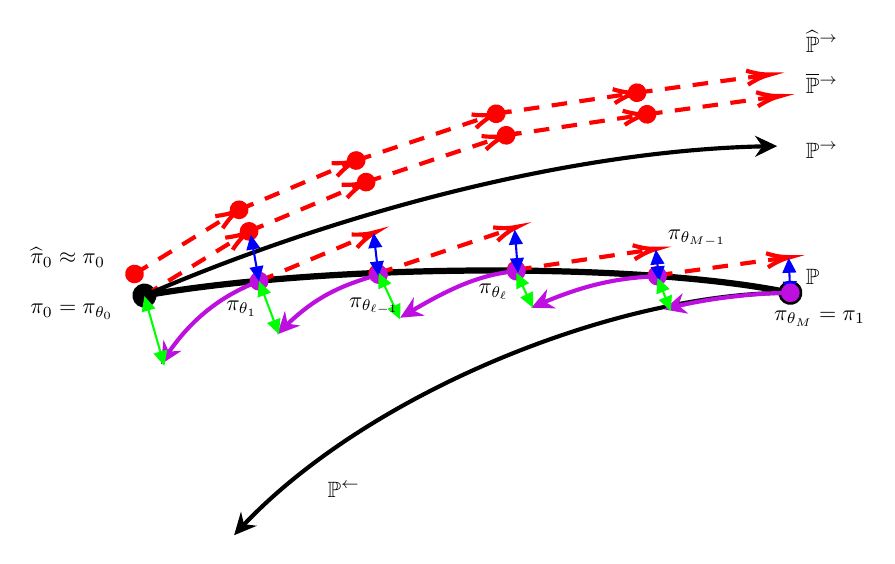
\begin{tikzpicture}[x=0.75pt,y=0.75pt,yscale=-0.8,xscale=0.8,every node/.style={scale=0.8}]
\draw [color={rgb, 255:red, 0; green, 0; blue, 0 }  ,draw opacity=1 ][line width=2.25]    (82,179.33) .. controls (190,160.33) and (379,158.67) .. (471,177.67) ;
\draw [shift={(471,177.67)}, rotate = 11.67] [color={rgb, 255:red, 0; green, 0; blue, 0 }  ,draw opacity=1 ][fill={rgb, 255:red, 0; green, 0; blue, 0 }  ,fill opacity=1 ][line width=2.25]      (0, 0) circle [x radius= 5.36, y radius= 5.36]   ;
\draw [shift={(82,179.33)}, rotate = 350.02] [color={rgb, 255:red, 0; green, 0; blue, 0 }  ,draw opacity=1 ][fill={rgb, 255:red, 0; green, 0; blue, 0 }  ,fill opacity=1 ][line width=2.25]      (0, 0) circle [x radius= 5.36, y radius= 5.36]   ;
\draw [color={rgb, 255:red, 255; green, 0; blue, 0 }  ,draw opacity=1 ][line width=1.5]  [dash pattern={on 5.63pt off 4.5pt}]  (82,179.33) -- (142.44,142.24) ;
\draw [shift={(145,140.67)}, rotate = 148.46] [color={rgb, 255:red, 255; green, 0; blue, 0 }  ,draw opacity=1 ][line width=1.5]    (14.21,-4.28) .. controls (9.04,-1.82) and (4.3,-0.39) .. (0,0) .. controls (4.3,0.39) and (9.04,1.82) .. (14.21,4.28)   ;
\draw [color={rgb, 255:red, 255; green, 0; blue, 0 }  ,draw opacity=1 ][line width=1.5]  [dash pattern={on 5.63pt off 4.5pt}]  (145,140.67) -- (212.73,112.16) ;
\draw [shift={(215.5,111)}, rotate = 157.18] [color={rgb, 255:red, 255; green, 0; blue, 0 }  ,draw opacity=1 ][line width=1.5]    (14.21,-4.28) .. controls (9.04,-1.82) and (4.3,-0.39) .. (0,0) .. controls (4.3,0.39) and (9.04,1.82) .. (14.21,4.28)   ;
\draw [shift={(145,140.67)}, rotate = 337.18] [color={rgb, 255:red, 255; green, 0; blue, 0 }  ,draw opacity=1 ][fill={rgb, 255:red, 255; green, 0; blue, 0 }  ,fill opacity=1 ][line width=1.5]      (0, 0) circle [x radius= 4.36, y radius= 4.36]   ;
\draw [color={rgb, 255:red, 255; green, 0; blue, 0 }  ,draw opacity=1 ][line width=1.5]  [dash pattern={on 5.63pt off 4.5pt}]  (215.5,111) -- (296.99,83.78) ;
\draw [shift={(299.83,82.83)}, rotate = 161.53] [color={rgb, 255:red, 255; green, 0; blue, 0 }  ,draw opacity=1 ][line width=1.5]    (14.21,-4.28) .. controls (9.04,-1.82) and (4.3,-0.39) .. (0,0) .. controls (4.3,0.39) and (9.04,1.82) .. (14.21,4.28)   ;
\draw [shift={(215.5,111)}, rotate = 341.53] [color={rgb, 255:red, 255; green, 0; blue, 0 }  ,draw opacity=1 ][fill={rgb, 255:red, 255; green, 0; blue, 0 }  ,fill opacity=1 ][line width=1.5]      (0, 0) circle [x radius= 4.36, y radius= 4.36]   ;
\draw [color={rgb, 255:red, 255; green, 0; blue, 0 }  ,draw opacity=1 ][line width=1.5]  [dash pattern={on 5.63pt off 4.5pt}]  (299.83,82.83) -- (381.7,70.61) ;
\draw [shift={(384.67,70.17)}, rotate = 171.51] [color={rgb, 255:red, 255; green, 0; blue, 0 }  ,draw opacity=1 ][line width=1.5]    (14.21,-4.28) .. controls (9.04,-1.82) and (4.3,-0.39) .. (0,0) .. controls (4.3,0.39) and (9.04,1.82) .. (14.21,4.28)   ;
\draw [shift={(299.83,82.83)}, rotate = 351.51] [color={rgb, 255:red, 255; green, 0; blue, 0 }  ,draw opacity=1 ][fill={rgb, 255:red, 255; green, 0; blue, 0 }  ,fill opacity=1 ][line width=1.5]      (0, 0) circle [x radius= 4.36, y radius= 4.36]   ;
\draw [color={rgb, 255:red, 255; green, 0; blue, 0 }  ,draw opacity=1 ][line width=1.5]  [dash pattern={on 5.63pt off 4.5pt}]  (384.67,70.17) -- (462.03,59.57) ;
\draw [shift={(465,59.17)}, rotate = 172.2] [color={rgb, 255:red, 255; green, 0; blue, 0 }  ,draw opacity=1 ][line width=1.5]    (14.21,-4.28) .. controls (9.04,-1.82) and (4.3,-0.39) .. (0,0) .. controls (4.3,0.39) and (9.04,1.82) .. (14.21,4.28)   ;
\draw [shift={(384.67,70.17)}, rotate = 352.2] [color={rgb, 255:red, 255; green, 0; blue, 0 }  ,draw opacity=1 ][fill={rgb, 255:red, 255; green, 0; blue, 0 }  ,fill opacity=1 ][line width=1.5]      (0, 0) circle [x radius= 4.36, y radius= 4.36]   ;
\draw [color={rgb, 255:red, 0; green, 0; blue, 0 }  ,draw opacity=1 ][line width=1.5]    (82,179.33) .. controls (186.94,133.79) and (334.02,91.19) .. (459.21,89.38) ;
\draw [shift={(463,89.33)}, rotate = 179.55] [fill={rgb, 255:red, 0; green, 0; blue, 0 }  ,fill opacity=1 ][line width=0.08]  [draw opacity=0] (13.4,-6.43) -- (0,0) -- (13.4,6.44) -- (8.9,0) -- cycle    ;
\draw [shift={(82,179.33)}, rotate = 336.54] [color={rgb, 255:red, 0; green, 0; blue, 0 }  ,draw opacity=1 ][fill={rgb, 255:red, 0; green, 0; blue, 0 }  ,fill opacity=1 ][line width=1.5]      (0, 0) circle [x radius= 4.36, y radius= 4.36]   ;
\draw [color={rgb, 255:red, 0; green, 0; blue, 0 }  ,draw opacity=1 ][line width=1.5]    (139.43,319.9) .. controls (215.61,237.81) and (366.59,177.34) .. (471,177.67) ;
\draw [shift={(471,177.67)}, rotate = 0.18] [color={rgb, 255:red, 0; green, 0; blue, 0 }  ,draw opacity=1 ][fill={rgb, 255:red, 0; green, 0; blue, 0 }  ,fill opacity=1 ][line width=1.5]      (0, 0) circle [x radius= 4.36, y radius= 4.36]   ;
\draw [shift={(136,323.67)}, rotate = 311.76] [fill={rgb, 255:red, 0; green, 0; blue, 0 }  ,fill opacity=1 ][line width=0.08]  [draw opacity=0] (13.4,-6.43) -- (0,0) -- (13.4,6.44) -- (8.9,0) -- cycle    ;
\draw [color={rgb, 255:red, 255; green, 0; blue, 0 }  ,draw opacity=1 ][line width=1.5]  [dash pattern={on 5.63pt off 4.5pt}]  (76,166.33) -- (136.44,129.24) ;
\draw [shift={(139,127.67)}, rotate = 148.46] [color={rgb, 255:red, 255; green, 0; blue, 0 }  ,draw opacity=1 ][line width=1.5]    (14.21,-4.28) .. controls (9.04,-1.82) and (4.3,-0.39) .. (0,0) .. controls (4.3,0.39) and (9.04,1.82) .. (14.21,4.28)   ;
\draw [shift={(76,166.33)}, rotate = 328.46] [color={rgb, 255:red, 255; green, 0; blue, 0 }  ,draw opacity=1 ][fill={rgb, 255:red, 255; green, 0; blue, 0 }  ,fill opacity=1 ][line width=1.5]      (0, 0) circle [x radius= 4.36, y radius= 4.36]   ;
\draw [color={rgb, 255:red, 255; green, 0; blue, 0 }  ,draw opacity=1 ][line width=1.5]  [dash pattern={on 5.63pt off 4.5pt}]  (139,127.67) -- (206.73,99.16) ;
\draw [shift={(209.5,98)}, rotate = 157.18] [color={rgb, 255:red, 255; green, 0; blue, 0 }  ,draw opacity=1 ][line width=1.5]    (14.21,-4.28) .. controls (9.04,-1.82) and (4.3,-0.39) .. (0,0) .. controls (4.3,0.39) and (9.04,1.82) .. (14.21,4.28)   ;
\draw [shift={(139,127.67)}, rotate = 337.18] [color={rgb, 255:red, 255; green, 0; blue, 0 }  ,draw opacity=1 ][fill={rgb, 255:red, 255; green, 0; blue, 0 }  ,fill opacity=1 ][line width=1.5]      (0, 0) circle [x radius= 4.36, y radius= 4.36]   ;
\draw [color={rgb, 255:red, 255; green, 0; blue, 0 }  ,draw opacity=1 ][line width=1.5]  [dash pattern={on 5.63pt off 4.5pt}]  (209.5,98) -- (290.99,70.78) ;
\draw [shift={(293.83,69.83)}, rotate = 161.53] [color={rgb, 255:red, 255; green, 0; blue, 0 }  ,draw opacity=1 ][line width=1.5]    (14.21,-4.28) .. controls (9.04,-1.82) and (4.3,-0.39) .. (0,0) .. controls (4.3,0.39) and (9.04,1.82) .. (14.21,4.28)   ;
\draw [shift={(209.5,98)}, rotate = 341.53] [color={rgb, 255:red, 255; green, 0; blue, 0 }  ,draw opacity=1 ][fill={rgb, 255:red, 255; green, 0; blue, 0 }  ,fill opacity=1 ][line width=1.5]      (0, 0) circle [x radius= 4.36, y radius= 4.36]   ;
\draw [color={rgb, 255:red, 255; green, 0; blue, 0 }  ,draw opacity=1 ][line width=1.5]  [dash pattern={on 5.63pt off 4.5pt}]  (293.83,69.83) -- (375.7,57.61) ;
\draw [shift={(378.67,57.17)}, rotate = 171.51] [color={rgb, 255:red, 255; green, 0; blue, 0 }  ,draw opacity=1 ][line width=1.5]    (14.21,-4.28) .. controls (9.04,-1.82) and (4.3,-0.39) .. (0,0) .. controls (4.3,0.39) and (9.04,1.82) .. (14.21,4.28)   ;
\draw [shift={(293.83,69.83)}, rotate = 351.51] [color={rgb, 255:red, 255; green, 0; blue, 0 }  ,draw opacity=1 ][fill={rgb, 255:red, 255; green, 0; blue, 0 }  ,fill opacity=1 ][line width=1.5]      (0, 0) circle [x radius= 4.36, y radius= 4.36]   ;
\draw [color={rgb, 255:red, 255; green, 0; blue, 0 }  ,draw opacity=1 ][line width=1.5]  [dash pattern={on 5.63pt off 4.5pt}]  (378.67,57.17) -- (456.03,46.57) ;
\draw [shift={(459,46.17)}, rotate = 172.2] [color={rgb, 255:red, 255; green, 0; blue, 0 }  ,draw opacity=1 ][line width=1.5]    (14.21,-4.28) .. controls (9.04,-1.82) and (4.3,-0.39) .. (0,0) .. controls (4.3,0.39) and (9.04,1.82) .. (14.21,4.28)   ;
\draw [shift={(378.67,57.17)}, rotate = 352.2] [color={rgb, 255:red, 255; green, 0; blue, 0 }  ,draw opacity=1 ][fill={rgb, 255:red, 255; green, 0; blue, 0 }  ,fill opacity=1 ][line width=1.5]      (0, 0) circle [x radius= 4.36, y radius= 4.36]   ;
\draw [color={rgb, 255:red, 255; green, 0; blue, 0 }  ,draw opacity=1 ][line width=1.5]  [dash pattern={on 5.63pt off 4.5pt}]  (151,170.67) -- (218.73,142.16) ;
\draw [shift={(221.5,141)}, rotate = 157.18] [color={rgb, 255:red, 255; green, 0; blue, 0 }  ,draw opacity=1 ][line width=1.5]    (14.21,-4.28) .. controls (9.04,-1.82) and (4.3,-0.39) .. (0,0) .. controls (4.3,0.39) and (9.04,1.82) .. (14.21,4.28)   ;
\draw [shift={(151,170.67)}, rotate = 337.18] [color={rgb, 255:red, 255; green, 0; blue, 0 }  ,draw opacity=1 ][fill={rgb, 255:red, 255; green, 0; blue, 0 }  ,fill opacity=1 ][line width=1.5]      (0, 0) circle [x radius= 4.36, y radius= 4.36]   ;
\draw [color={rgb, 255:red, 255; green, 0; blue, 0 }  ,draw opacity=1 ][line width=1.5]  [dash pattern={on 5.63pt off 4.5pt}]  (222.5,166) -- (303.99,138.78) ;
\draw [shift={(306.83,137.83)}, rotate = 161.53] [color={rgb, 255:red, 255; green, 0; blue, 0 }  ,draw opacity=1 ][line width=1.5]    (14.21,-4.28) .. controls (9.04,-1.82) and (4.3,-0.39) .. (0,0) .. controls (4.3,0.39) and (9.04,1.82) .. (14.21,4.28)   ;
\draw [shift={(222.5,166)}, rotate = 341.53] [color={rgb, 255:red, 255; green, 0; blue, 0 }  ,draw opacity=1 ][fill={rgb, 255:red, 255; green, 0; blue, 0 }  ,fill opacity=1 ][line width=1.5]      (0, 0) circle [x radius= 4.36, y radius= 4.36]   ;
\draw [color={rgb, 255:red, 255; green, 0; blue, 0 }  ,draw opacity=1 ][line width=1.5]  [dash pattern={on 5.63pt off 4.5pt}]  (305.83,163.83) -- (387.7,151.61) ;
\draw [shift={(390.67,151.17)}, rotate = 171.51] [color={rgb, 255:red, 255; green, 0; blue, 0 }  ,draw opacity=1 ][line width=1.5]    (14.21,-4.28) .. controls (9.04,-1.82) and (4.3,-0.39) .. (0,0) .. controls (4.3,0.39) and (9.04,1.82) .. (14.21,4.28)   ;
\draw [shift={(305.83,163.83)}, rotate = 351.51] [color={rgb, 255:red, 255; green, 0; blue, 0 }  ,draw opacity=1 ][fill={rgb, 255:red, 255; green, 0; blue, 0 }  ,fill opacity=1 ][line width=1.5]      (0, 0) circle [x radius= 4.36, y radius= 4.36]   ;
\draw [color={rgb, 255:red, 255; green, 0; blue, 0 }  ,draw opacity=1 ][line width=1.5]  [dash pattern={on 5.63pt off 4.5pt}]  (390.67,167.17) -- (468.03,156.57) ;
\draw [shift={(471,156.17)}, rotate = 172.2] [color={rgb, 255:red, 255; green, 0; blue, 0 }  ,draw opacity=1 ][line width=1.5]    (14.21,-4.28) .. controls (9.04,-1.82) and (4.3,-0.39) .. (0,0) .. controls (4.3,0.39) and (9.04,1.82) .. (14.21,4.28)   ;
\draw [shift={(390.67,167.17)}, rotate = 352.2] [color={rgb, 255:red, 255; green, 0; blue, 0 }  ,draw opacity=1 ][fill={rgb, 255:red, 255; green, 0; blue, 0 }  ,fill opacity=1 ][line width=1.5]      (0, 0) circle [x radius= 4.36, y radius= 4.36]   ;
\draw [color={rgb, 255:red, 189; green, 16; blue, 224 }  ,draw opacity=1 ][line width=1.5]    (318.87,184.96) .. controls (345.9,173.22) and (366.17,168.62) .. (391,167.67) ;
\draw [shift={(391,167.67)}, rotate = 357.8] [color={rgb, 255:red, 189; green, 16; blue, 224 }  ,draw opacity=1 ][fill={rgb, 255:red, 189; green, 16; blue, 224 }  ,fill opacity=1 ][line width=1.5]      (0, 0) circle [x radius= 4.36, y radius= 4.36]   ;
\draw [shift={(315,186.67)}, rotate = 335.85] [fill={rgb, 255:red, 189; green, 16; blue, 224 }  ,fill opacity=1 ][line width=0.08]  [draw opacity=0] (13.4,-6.43) -- (0,0) -- (13.4,6.44) -- (8.9,0) -- cycle    ;
\draw [color={rgb, 255:red, 189; green, 16; blue, 224 }  ,draw opacity=1 ][line width=1.5]    (239.63,190.52) .. controls (260.43,178.27) and (281.43,166.56) .. (306,164.67) ;
\draw [shift={(306,164.67)}, rotate = 355.6] [color={rgb, 255:red, 189; green, 16; blue, 224 }  ,draw opacity=1 ][fill={rgb, 255:red, 189; green, 16; blue, 224 }  ,fill opacity=1 ][line width=1.5]      (0, 0) circle [x radius= 4.36, y radius= 4.36]   ;
\draw [shift={(236,192.67)}, rotate = 329.42] [fill={rgb, 255:red, 189; green, 16; blue, 224 }  ,fill opacity=1 ][line width=0.08]  [draw opacity=0] (13.4,-6.43) -- (0,0) -- (13.4,6.44) -- (8.9,0) -- cycle    ;
\draw [color={rgb, 255:red, 189; green, 16; blue, 224 }  ,draw opacity=1 ][line width=1.5]    (164.81,199.79) .. controls (184.46,180.04) and (200.08,173.35) .. (223,166.67) ;
\draw [shift={(223,166.67)}, rotate = 343.74] [color={rgb, 255:red, 189; green, 16; blue, 224 }  ,draw opacity=1 ][fill={rgb, 255:red, 189; green, 16; blue, 224 }  ,fill opacity=1 ][line width=1.5]      (0, 0) circle [x radius= 4.36, y radius= 4.36]   ;
\draw [shift={(162,202.67)}, rotate = 313.67] [fill={rgb, 255:red, 189; green, 16; blue, 224 }  ,fill opacity=1 ][line width=0.08]  [draw opacity=0] (13.4,-6.43) -- (0,0) -- (13.4,6.44) -- (8.9,0) -- cycle    ;
\draw [color={rgb, 255:red, 189; green, 16; blue, 224 }  ,draw opacity=1 ][line width=1.5]    (94.32,216.97) .. controls (110.89,191.42) and (130.95,178.31) .. (151,170.67) ;
\draw [shift={(151,170.67)}, rotate = 339.15] [color={rgb, 255:red, 189; green, 16; blue, 224 }  ,draw opacity=1 ][fill={rgb, 255:red, 189; green, 16; blue, 224 }  ,fill opacity=1 ][line width=1.5]      (0, 0) circle [x radius= 4.36, y radius= 4.36]   ;
\draw [shift={(92,220.67)}, rotate = 301.26] [fill={rgb, 255:red, 189; green, 16; blue, 224 }  ,fill opacity=1 ][line width=0.08]  [draw opacity=0] (13.4,-6.43) -- (0,0) -- (13.4,6.44) -- (8.9,0) -- cycle    ;
\draw [color={rgb, 255:red, 0; green, 0; blue, 255 }  ,draw opacity=1 ][line width=0.75]    (146.53,145.62) -- (150.47,167.71) ;
\draw [shift={(151,170.67)}, rotate = 259.88] [fill={rgb, 255:red, 0; green, 0; blue, 255 }  ,fill opacity=1 ][line width=0.08]  [draw opacity=0] (8.93,-4.29) -- (0,0) -- (8.93,4.29) -- cycle    ;
\draw [shift={(146,142.67)}, rotate = 79.88] [fill={rgb, 255:red, 0; green, 0; blue, 255 }  ,fill opacity=1 ][line width=0.08]  [draw opacity=0] (8.93,-4.29) -- (0,0) -- (8.93,4.29) -- cycle    ;
\draw [color={rgb, 255:red, 0; green, 0; blue, 255 }  ,draw opacity=1 ][line width=0.75]    (220.34,144.65) -- (222.66,164.69) ;
\draw [shift={(223,167.67)}, rotate = 263.42] [fill={rgb, 255:red, 0; green, 0; blue, 255 }  ,fill opacity=1 ][line width=0.08]  [draw opacity=0] (8.93,-4.29) -- (0,0) -- (8.93,4.29) -- cycle    ;
\draw [shift={(220,141.67)}, rotate = 83.42] [fill={rgb, 255:red, 0; green, 0; blue, 255 }  ,fill opacity=1 ][line width=0.08]  [draw opacity=0] (8.93,-4.29) -- (0,0) -- (8.93,4.29) -- cycle    ;
\draw [color={rgb, 255:red, 0; green, 0; blue, 255 }  ,draw opacity=1 ][line width=0.75]    (305.23,142.66) -- (306.77,162.68) ;
\draw [shift={(307,165.67)}, rotate = 265.6] [fill={rgb, 255:red, 0; green, 0; blue, 255 }  ,fill opacity=1 ][line width=0.08]  [draw opacity=0] (8.93,-4.29) -- (0,0) -- (8.93,4.29) -- cycle    ;
\draw [shift={(305,139.67)}, rotate = 85.6] [fill={rgb, 255:red, 0; green, 0; blue, 255 }  ,fill opacity=1 ][line width=0.08]  [draw opacity=0] (8.93,-4.29) -- (0,0) -- (8.93,4.29) -- cycle    ;
\draw [color={rgb, 255:red, 0; green, 0; blue, 255 }  ,draw opacity=1 ][line width=0.75]    (390.31,154.65) -- (391.69,167.68) ;
\draw [shift={(392,170.67)}, rotate = 263.99] [fill={rgb, 255:red, 0; green, 0; blue, 255 }  ,fill opacity=1 ][line width=0.08]  [draw opacity=0] (8.93,-4.29) -- (0,0) -- (8.93,4.29) -- cycle    ;
\draw [shift={(390,151.67)}, rotate = 83.99] [fill={rgb, 255:red, 0; green, 0; blue, 255 }  ,fill opacity=1 ][line width=0.08]  [draw opacity=0] (8.93,-4.29) -- (0,0) -- (8.93,4.29) -- cycle    ;
\draw [color={rgb, 255:red, 0; green, 0; blue, 255 }  ,draw opacity=1 ][line width=0.75]    (470.13,159.66) -- (470.87,176.67) ;
\draw [shift={(471,179.67)}, rotate = 267.51] [fill={rgb, 255:red, 0; green, 0; blue, 255 }  ,fill opacity=1 ][line width=0.08]  [draw opacity=0] (8.93,-4.29) -- (0,0) -- (8.93,4.29) -- cycle    ;
\draw [shift={(470,156.67)}, rotate = 87.51] [fill={rgb, 255:red, 0; green, 0; blue, 255 }  ,fill opacity=1 ][line width=0.08]  [draw opacity=0] (8.93,-4.29) -- (0,0) -- (8.93,4.29) -- cycle    ;
\draw [color={rgb, 255:red, 0; green, 255; blue, 0 }  ,draw opacity=1 ][line width=0.75]    (82.82,182.55) -- (93.18,218.78) ;
\draw [shift={(94,221.67)}, rotate = 254.05] [fill={rgb, 255:red, 0; green, 255; blue, 0 }  ,fill opacity=1 ][line width=0.08]  [draw opacity=0] (8.93,-4.29) -- (0,0) -- (8.93,4.29) -- cycle    ;
\draw [shift={(82,179.67)}, rotate = 74.05] [fill={rgb, 255:red, 0; green, 255; blue, 0 }  ,fill opacity=1 ][line width=0.08]  [draw opacity=0] (8.93,-4.29) -- (0,0) -- (8.93,4.29) -- cycle    ;
\draw [color={rgb, 255:red, 0; green, 255; blue, 0 }  ,draw opacity=1 ][line width=0.75]    (152.05,173.48) -- (161.95,199.86) ;
\draw [shift={(163,202.67)}, rotate = 249.44] [fill={rgb, 255:red, 0; green, 255; blue, 0 }  ,fill opacity=1 ][line width=0.08]  [draw opacity=0] (8.93,-4.29) -- (0,0) -- (8.93,4.29) -- cycle    ;
\draw [shift={(151,170.67)}, rotate = 69.44] [fill={rgb, 255:red, 0; green, 255; blue, 0 }  ,fill opacity=1 ][line width=0.08]  [draw opacity=0] (8.93,-4.29) -- (0,0) -- (8.93,4.29) -- cycle    ;
\draw [color={rgb, 255:red, 0; green, 255; blue, 0 }  ,draw opacity=1 ][line width=0.75]    (224.26,168.39) -- (234.74,190.95) ;
\draw [shift={(236,193.67)}, rotate = 245.1] [fill={rgb, 255:red, 0; green, 255; blue, 0 }  ,fill opacity=1 ][line width=0.08]  [draw opacity=0] (8.93,-4.29) -- (0,0) -- (8.93,4.29) -- cycle    ;
\draw [shift={(223,165.67)}, rotate = 65.1] [fill={rgb, 255:red, 0; green, 255; blue, 0 }  ,fill opacity=1 ][line width=0.08]  [draw opacity=0] (8.93,-4.29) -- (0,0) -- (8.93,4.29) -- cycle    ;
\draw [color={rgb, 255:red, 0; green, 255; blue, 0 }  ,draw opacity=1 ][line width=0.75]    (307.29,168.38) -- (314.71,183.96) ;
\draw [shift={(316,186.67)}, rotate = 244.54] [fill={rgb, 255:red, 0; green, 255; blue, 0 }  ,fill opacity=1 ][line width=0.08]  [draw opacity=0] (8.93,-4.29) -- (0,0) -- (8.93,4.29) -- cycle    ;
\draw [shift={(306,165.67)}, rotate = 64.54] [fill={rgb, 255:red, 0; green, 255; blue, 0 }  ,fill opacity=1 ][line width=0.08]  [draw opacity=0] (8.93,-4.29) -- (0,0) -- (8.93,4.29) -- cycle    ;
\draw [color={rgb, 255:red, 189; green, 16; blue, 224 }  ,draw opacity=1 ][line width=1.5]    (399.19,186.55) .. controls (423.58,180.35) and (453.99,177.67) .. (471,177.67) ;
\draw [shift={(471,177.67)}, rotate = 0] [color={rgb, 255:red, 189; green, 16; blue, 224 }  ,draw opacity=1 ][fill={rgb, 255:red, 189; green, 16; blue, 224 }  ,fill opacity=1 ][line width=1.5]      (0, 0) circle [x radius= 4.36, y radius= 4.36]   ;
\draw [shift={(395,187.67)}, rotate = 344.36] [fill={rgb, 255:red, 189; green, 16; blue, 224 }  ,fill opacity=1 ][line width=0.08]  [draw opacity=0] (13.4,-6.43) -- (0,0) -- (13.4,6.44) -- (8.9,0) -- cycle    ;
\draw [color={rgb, 255:red, 0; green, 255; blue, 0 }  ,draw opacity=1 ][line width=0.75]    (392.11,171.45) -- (397.89,185.88) ;
\draw [shift={(399,188.67)}, rotate = 248.2] [fill={rgb, 255:red, 0; green, 255; blue, 0 }  ,fill opacity=1 ][line width=0.08]  [draw opacity=0] (8.93,-4.29) -- (0,0) -- (8.93,4.29) -- cycle    ;
\draw [shift={(391,168.67)}, rotate = 68.2] [fill={rgb, 255:red, 0; green, 255; blue, 0 }  ,fill opacity=1 ][line width=0.08]  [draw opacity=0] (8.93,-4.29) -- (0,0) -- (8.93,4.29) -- cycle    ;

\draw (12,183.33) node [anchor=north west][inner sep=0.75pt]   [align=left] {$\displaystyle \pi _{0} =\pi _{\theta _{0}}$};
\draw (130,181.33) node [anchor=north west][inner sep=0.75pt]   [align=left] {$\displaystyle \pi _{\theta _{1}}$};
\draw (396,138.33) node [anchor=north west][inner sep=0.75pt]   [align=left] {$\displaystyle \pi _{\theta _{M-1}}$};
\draw (460,187.33) node [anchor=north west][inner sep=0.75pt]   [align=left] {$\displaystyle \pi _{\theta _{M}} =\pi _{1}$};
\draw (191,290.33) node [anchor=north west][inner sep=0.75pt]   [align=left] {$\displaystyle \mathbb{P}^{\leftarrow }$};
\draw (479,86.33) node [anchor=north west][inner sep=0.75pt]   [align=left] {$\displaystyle \mathbb{P^{\rightarrow }}$};
\draw (479,44.33) node [anchor=north west][inner sep=0.75pt]   [align=left] {$\displaystyle \overline{\mathbb{P}}\mathbb{^{\rightarrow }}$};
\draw (479,162.33) node [anchor=north west][inner sep=0.75pt]   [align=left] {$\displaystyle \mathbb{P}$};
\draw (479,18.33) node [anchor=north west][inner sep=0.75pt]   [align=left] {$\displaystyle \mathbb{\widehat{P}^{\rightarrow }}$};
\draw (12,149.33) node [anchor=north west][inner sep=0.75pt]   [align=left] {$\displaystyle \widehat{\pi }_{0} \approx \pi _{0}$};
\draw (204,179.33) node [anchor=north west][inner sep=0.75pt]   [align=left] {$\displaystyle \pi _{\theta _{\ell -1}}$};
\draw (282,171.33) node [anchor=north west][inner sep=0.75pt]   [align=left] {$\displaystyle \pi _{\theta _{\ell }}$};

\end{tikzpicture}
    \caption{
    Illustration of the proof idea for \cref{thm:ais_complexity}.}
    \label{fig:prf_idea}
\end{figure}

\begin{enumerate}[wide=0pt,itemsep=0pt, topsep=0pt,parsep=0pt,partopsep=0pt]
    \item Analogously to the analysis of JE (\cref{thm:jar_complexity}), define the reference path measure $\P$ with transition kernels $F^*_\l$ such that $x_\l\sim\pi_{\theta_\l}$.
    Given the sampling path measure $\Phr$, define $\Pbr$ as the version of $\Phr$ without the initialization error, i.e., by replacing $\pih_0$ with $\pi_0$ in \cref{eq:ais_phr}. 
    \item Show that it suffices to obtain an accurate estimate $\Zh_0$ and initialization distribution $\pih_0$, together with sufficiently small KL divergences $\kl(\P\|\Pl)$ and $\kl(\P\|\Pbr)$, which quantify the closeness between the continuous dynamics and the discretization error in implementation, respectively.
    \item Using the chain rule, decompose $\kl(\P\|\Pl)$ into the sum of KL divergences between each pair of transition kernels $F_\l$ and $F^*_\l$ (i.e., the sum of \green{green} ``distances''). As in the proof of the convergence of JE (\cref{thm:jar_complexity}), $F^*_\l$, a transition kernel from $\pi_{\theta_{\l-1}}$ to $\pi_{\theta_\l}$, is realized by ALD with a compensatory vector field, ensuring the SDE exactly follows the trajectory $(\pi_\theta)_{\theta\in[\theta_{\l-1},\theta_\l]}$. 
    Similarly, by applying the chain rule and Girsanov theorem, we can express $\kl(\P\|\Pbr)$ as the sum of the \blue{blue} ``distances'', allowing for a similar analysis.
    \item Finally, derive three necessary conditions on the time steps $\theta_{\l}$ to control both $\kl(\P\|\Pl)$ and $\kl(\P\|\Pbr)$. Choosing a proper schedule yields the desired complexity bound.
\end{enumerate}

Our proposed algorithm consists of two phases: first, estimating $Z_0$ by TI, which is provably efficient for well-conditioned distributions, and second, estimating $Z$ by AIS, which is better suited for handling non-log-concave distributions. 
The three terms in \cref{eq:ais_complexity} arise from (i) ensuring the accuracy of $\Zh_0$, (ii) controlling $\kl(\P\|\Pl)$, and (iii) controlling $\kl(\P\|\Pbr)$, respectively, as discussed in \textbf{2.} above.
Due to the non-log-concavity of $\pi$, the action $\cA$ is typically large, making (iii), the cost for controlling the discretization error, the dominant complexity.
Finally, the $\varepsilon$-dependence can be interpreted as the total duration $T=\Theta\ro{\frac{1}{\varepsilon^2}}$ required for the continuous dynamics to converge (as in \cref{thm:jar_complexity}) divided by the step size $\Thetat(\varepsilon^2)$ to control the discretization error.
\section{Normalizing Constant Estimation via Reverse Diffusion Sampler}
\label{sec:revdif}
From the analysis of JE and AIS (\cref{thm:jar_complexity,thm:ais_complexity}), the choice of the interpolation curve $(\pi_\theta)_{\theta\in[0,1]}$ is crucial for the complexity of AIS. The geometric interpolation (\cref{eq:pi_theta}) is widely adopted in practice due to the availability of closed-form scores of the intermediate distributions $\pi_\theta$. For certain structured non-log-concave distributions, the associated action is polynomial in the problem parameters, enabling efficient AIS. For instance, \citet[Ex. 2]{guo2025provable} analyzed a Gaussian mixture target distribution with identical covariance, means having the \textit{same} norm, and arbitrary weights. However, for general target distributions, the action of the related curve can grow prohibitively large. To illustrate this, we establish an exponential lower bound on the action of a curve starting from a Gaussian mixture, highlighting the potential inefficiency of AIS under geometric interpolation. Our key technical tool is a closed-form expression of the $\text{W}_\text{2}$ distance in $\R$ expressed by the inverse cumulative distribution functions (c.d.f.s) of the involved distributions. We then lower bound the metric derivative near the target distribution, where the curve changes the most drastically. The proof of this result is detailed in \cref{app:prf:mog_w2_action}.

\begin{proposition}
    Consider the Gaussian mixture target distribution $\pi=\frac{1}{2}\n{0,1}+\frac{1}{2}\n{m,1}$ on $\R$ for some sufficiently large $m\gtrsim1$, whose potential is $\frac{m^2}{2}$-smooth. Under the setting in AIS (\cref{thm:ais_complexity}), define $\pi_\theta(x)\propto\pi(x)\e^{-\frac{\lambda(\theta)}{2}x^2}$, $\theta\in[0,1]$, where $\lambda(\theta)=m^2(1-\theta)^r$ for some $1\le r\lesssim1$. Then, the action of the curve $(\pi_\theta)_{\theta\in[0,1]}$ is lower bounded by $\cA_r\gtrsim m^{4}\e^{\frac{m^2}{40}}$.
    \label{thm:mog_w2_action}
\end{proposition}

Motivated by RDS, we propose leveraging the curve along the OU process in AIS. To support this idea, we first present the following proposition, whose proof is available in \cref{app:prf:action_ou}.

\begin{proposition}
    Let $\pib_t$ be the law of $Y_t$ in the OU process (\cref{eq:ou}) initialized from $Y_0\sim\pi\propto\e^{-V}$, where $V$ is $\beta$-smooth and let $m^2:=\E_\pi\|\cdot\|^2<\infty$. Then, $\int_0^\infty|\dot\pib|^2_t\d t\le d\beta+m^2$.
    \label{thm:action_ou}
\end{proposition}

This proposition shows that under fairly weak conditions on the target distribution, the action of the curve along the OU process, $(\pib_{T-t})_{t\in[0,T]}$, behaves much better than \cref{eq:pi_theta}. Hence, our analysis of JE (\cref{thm:jar_complexity}) suggests that this curve is likely to yield more efficient normalizing constant estimation. Furthermore, recall that in our earlier proof, we introduced a compensatory drift term $v_t$ to eliminate the lag in ALD. The same principle applies here: ensuring $X_t$ precisely following the reference trajectory is advantageous, which results in the time-reversal of OU process (\cref{eq:ou_rev}). Building on this insight, we propose an RDS-based algorithm for normalizing constant estimation, and establish a framework for analyzing its oracle complexity. The proof is in \cref{app:prf:revdif}.

\begin{theorem}
    Assume a total time duration $T$, an early stopping time $\delta\ge0$, and discrete time points $0=t_0<t_1<...<t_N=T-\delta\le T$. For $t\in[0,T-\delta)$, let $t_-$ denote $t_k$ if $t\in[t_k,t_{k+1})$. Let $s_\cdot\approx\nabla\log\pib_\cdot$ be a score estimator, and $\phi=\n{0,I}$. Consider the following two SDEs on $[0,T-\delta]$ representing the sampling trajectory and the time-reversed OU process, respectively:
    \begin{align}
        \Qd:\quad&\d X_t=(X_t+2s_{T-t_-}(X_{t_-}))\d t+\sqrt{2}\d B_t,&X_0\sim\phi;\label{eq:ou_rev_score}\\
        \Q:\quad&\d X_t=(X_t+2\nabla\log\pib_{T-t}(X_t))\d t+\sqrt{2}\d B_t,&X_0\sim\pib_T.\nonumber
    \end{align}
    Let $\Zh:=\e^{-W(X)}$, $X\sim\Qd$ be the estimator of $Z$, where the functional $X\mapsto W(X)$ is defined as
    \begin{align*}
        \log\phi(X_0)+V(X_{T-\delta})+(T-\delta)d+\int_0^{T-\delta}\ro{\|s_{T-t_-}(X_{t_-})\|^2\d t+\sqrt{2}\inn{s_{T-t_-}(X_{t_-}),\d B_t}}.
    \end{align*}
    Then, to ensure $\Zh$ satisfies \cref{eq:acc_whp}, it suffices that $\kl(\Q\|\Qd)\lesssim\varepsilon^2$ and $\tv(\pi,\pib_\delta)\lesssim\varepsilon$.
    \label{thm:revdif}
\end{theorem}

For detailed implementation of this algorithm including the update rule in \cref{eq:ou_rev_score} and the computation of $W(X)$, see \cref{alg:rds}. To determine the overall complexity, we leverage existing results for RDS \citep{huang2024reverse,huang2024faster,he2024zeroth,vacher2025polynomial} to derive the oracle complexity to achieve $\kl(\Q\|\Qd)\lesssim\varepsilon^2$. When early stopping is needed (i.e., $\delta>0$), we establish in \cref{lem:ou_tv} that choosing $\delta\asymp\frac{\varepsilon^2}{\beta^2d^2}$ suffices to ensure $\varepsilon$-closeness in TV distance between $\pib_\delta$ and $\pi$, under weak assumptions similar to \cref{assu:pi}. The detailed complexity analysis is deferred to \cref{app:revdif_overall}.

As discussed, RDS can be viewed as an \emph{optimally compensated} ALD using the OU process as the trajectory. We conclude this section by contrasting these two approaches. On the one hand, analytically-tractable curves such as the geometric interpolation offer closed-form drift terms at all time points, but may exhibit poor action properties (\cref{thm:mog_w2_action}) or bad isoperimetric constants \citep{chehab2025provable}, making annealed sampling challenging. On the other hand, alternative curves like the OU process may have better properties in action and isoperimetric constants, but their drift terms, often related to the scores of the intermediate distributions, lack closed-form expressions, and estimating these terms is also non-trivial. This highlights a fundamental trade-off between the complexity of the drift term estimation and the property of the interpolation curve. 
\section{Conclusion and Future Work}
\label{sec:conc}
In this paper, we analyzed the complexity of normalizing constant estimation using JE, AIS, and RDS, establishing non-asymptotic convergence guarantees based on insights from continuous-time analysis. Our analysis of JE (\cref{thm:jar_complexity}) applies to general interpolation curves without requiring explicit isoperimetric assumptions, which significantly extends prior work limited to log-concave distributions. While our main results (\cref{thm:jar_complexity,thm:ais_complexity}) provide upper complexity bounds, their tightness remains an open question. Deriving general lower bounds would further clarify whether curves with large action inherently require more oracle calls for both sampling and normalizing constant estimation, thereby rigorously validating the arguments in \cref{sec:revdif}. We also conjecture that our proof techniques can be further extended to samplers beyond overdamped LD (e.g., Hamiltonian or underdamped LD \citep{sohl2012hamiltonian}), and may be applied to estimating normalizing constants of compactly supported distributions on $\R^d$ (e.g., convex bodies volume estimation \citep{cousins2018gaussian}) and discrete distributions (e.g., Ising model and restricted Boltzmann machines \citep{huber2015approximation,krause2020algorithms}) via the Poisson stochastic integral framework \citep{ren2025how,ren2025fast}. We leave these directions for future research.

\newpage
\bibliography{ref}

\newpage
\appendix
\tableofcontents
\newpage
\section{Preliminaries (Continued)}
\label{app:pre}
The theories of backward stochastic integral and the Girsanov theorem are adapted from \cite{vargas2024transport}. Here, we include relevant results and proofs to ensure a self-contained presentation.  

\begin{lemma}[Nelson's relation {\citep{nelson1967dynamical,anderson1982reversetime}}]
    \label{lem:nelson}
    Given a BM $(B_t)_{t\in[0,T]}$ and its time-reversal $(\Bl_t=B_{T-t})_{t\in[0,T]}$, the following two SDEs
    $$\d X_t=a_t(X_t)\d t+\sigma\d B_t,~X_0\sim p_0;~\d Y_t=b_t(Y_t)\d t+\sigma\d\Bl_t,~Y_T\sim q$$
    have the same path measure if and only if
    $$q=p_T,\quad\text{and}\quad b_t=a_t-\sigma^2\nabla\log p_t,~\forall t\in[0,T],$$
    where $p_t$ is the p.d.f. of $X_t$.
\end{lemma}

\begin{proof}
    The proof is by verifying the Fokker-Planck equation. For $X$, we have
    $$\partial_tp_t=-\nabla\cdot(a_tp_t)+\frac{\sigma^2}{2}\Delta p_t.$$
    Let $\star^\gets_t:=\star_{T-t}$. Then $\pl_t$ satisfies
    $$\partial_t\pl_t=\nabla\cdot(\al_t\pl_t)-\frac{\sigma^2}{2}\Delta\pl_t=-\nabla\cdot((-\al_t+\sigma^2\nabla\log\pl_t)\pl_t)+\frac{\sigma^2}{2}\Delta\pl_t,$$
    which means $(\Xl_t)_{t\in[0,T]}$ has the same path measure as the following SDE:
    $$\d Z_t=-(\al_t-\sigma^2\nabla\log\pl_t)(Z_t)\d t+\sigma\d B_t,~Z_t\sim\pl_t.$$
    On the other hand, by definition, $(\Yl_t)_{t\in[0,T]}$ satisfies the forward SDE
    $$\d\Yl_t=-\bl_t(\Yl_t)\d t+\sigma\d B_t,~Y_0\sim q,$$
    and thus the claim is evident.
\end{proof}

\begin{definition}[Backward stochastic integral]
    \label{def:bsi}
    For two continuous stochastic processes $X$ and $Y$ on $C([0,T];\R^d)$, the \textbf{backward stochastic integral} of $Y$ with respect to $X$ is defined as
    $$\int_0^T\inn{Y_t,*\d X_t}:=\prob\,{\text-}\lim_{\|\Pi\|\to0}\sum_{i=0}^{n-1}\inn{Y_{t_{i+1}},X_{t_{i+1}}-X_{t_i}},$$
    where $\Pi=\{0=t_0<t_1<...<t_n=T\}$ is a partition of $[0,T]$, $\|\Pi\|:=\max\limits_{i\in\sqd{1,n}}(t_{i+1}-t_i)$, and the convergence is in the probability sense. When both $X$ and $Y$ are continuous semi-martingales, one can equivalently define
    \begin{equation}
        \int_0^T\inn{Y_t,*\d X_t}:=\int_0^T\inn{Y_t,\d X_t}+[X,Y]_T,
        \label{eq:bsi_ito}
    \end{equation}
    where $[X,Y]_\cdot$ is the cross quadratic variation process\footnote{The notation used in \cite{karatzas1991brownian} is $\inn{\cdot,\cdot}_\cdot$. We use square brackets here to avoid conflict with the notation for inner product.} of the local martingale parts of $X$ and $Y$.
    \end{definition}

\begin{remark}
    Although rarely used in practice, the backward stochastic integral is sometimes referred to as the H\"anggi-Klimontovich integral in the literature. Recall that the It\^o integral is defined as the limit of Riemann sums when the leftmost point of each interval is used, while the Stratonovich integral is based on the midpoint and the backward integral uses the rightmost point. The equivalence in \cref{eq:bsi_ito} can be justified in \citet[Chap. 3.3]{karatzas1991brownian}. 
\end{remark}

\begin{lemma}[Continuation of \cref{lem:rn_path_measure}]
\begin{enumerate}[wide=0pt,itemsep=0pt, topsep=0pt,parsep=0pt,partopsep=0pt]
    \item If we replace the SDEs in \cref{lem:rn_path_measure} with
    $$\d X_t =a_t(X_t)\d t+\sigma\d\Bl_t,~X_T\sim\mu;\qquad\d Y_t =b_t(Y_t)\d t+\sigma\d\Bl_t,~Y_T\sim\nu,$$
    while keeping other assumptions and notations unchanged, then for any trajectory $\xi\in\Omega$, 
    \begin{align*}
        \log\de{\P^X}{\P^Y}(\xi) & =\log\de{\mu}{\nu}(\xi_T)+\frac{1}{\sigma^2}\int_0^T\inn{a_t(\xi_t)-b_t(\xi_t),*\d\xi_t}-\frac{1}{2\sigma^2}\int_0^T(\|a_t(\xi_t)\|^2-\|b_t(\xi_t)\|^2)\d t,
    \end{align*}
    and consequently, 
    $$\kl(\P^X\|\P^Y)=\kl(\mu\|\nu)+\frac{1}{2\sigma^2}\int_0^T\E_{\P^X}\|a_t(X_t)-b_t(X_t)\|^2\d t.$$

    \item Define the following two SDEs from $0$ to $T$:
    $$\d X_t =a_t(X_t)\d t+\sigma\d B_t,~X_0\sim\mu;\qquad\d Y_t =b_t(Y_t)\d t+\sigma\d\Bl_t,~Y_T\sim\nu.$$
    Denote the path measures of $X$ and $Y$ as $\P^X$ and $\P^Y$, respectively. Then for any trajectory $\xi\in\Omega$,
    \begin{align*}
        \log\de{\P^X}{\P^Y}(\xi) & =\log\frac{\mu(\xi_0)}{\nu(\xi_T)}+\frac{1}{\sigma^2}\int_0^T(\inn{a_t(\xi_t),\d\xi_t}-\inn{b_t(\xi_t),*\d\xi_t})-\frac{1}{2\sigma^2}\int_0^T(\|a_t(\xi_t)\|^2-\|b_t(\xi_t)\|^2)\d t.
    \end{align*}
\end{enumerate}
\label{lem:rn_path_measure_contd}
\end{lemma}

\begin{proof}
\begin{enumerate}[wide=0pt,itemsep=0pt, topsep=0pt,parsep=0pt,partopsep=0pt]
\item Let $\star^\gets_t:=\star_{T-t}$. We know that
$$\d\Xl_t =-\al_t(\Xl_t)\d t+\sigma\d B_t,~\Xl_0\sim\mu;\qquad\d\Yl_t =-\bl_t(\Yl_t)\d t+\sigma\d B_t,~\Yl_0\sim\nu.$$
Let $\P^{\Xl}$ and $\P^{\Yl}$ be the path measures of $\Xl$ and $\Yl$, respectively. From \cref{lem:rn_path_measure}, we know that
\begin{align*}
    \log\de{\P^{\Xl}}{\P^{\Yl}}(\xi) & =\log\de{\mu}{\nu}(\xi_0)-\frac{1}{\sigma^2}\int_0^T\inn{\al_t(\xi_t)-\bl_t(\xi_t),\d\xi_t}-\frac{1}{2\sigma^2}\int_0^T(\|\al_t(\xi_t)\|^2-\|\bl_t(\xi_t)\|^2)\d t.
\end{align*}
Since $\P^{\Xl}(\d\xi)=\prob(\Xl\in\d\xi)=\prob(X\in\d\xil)=\P^X(\d\xil)$, we obtain
\begin{align*}
    &\log\de{\P^X}{\P^Y}(\xi) =\log\de{\P^{\Xl}}{\P^{\Yl}}(\xil)\\
    &=\log\de{\mu}{\nu}(\xil_0)-\frac{1}{\sigma^2}\int_0^T\inn{\al_t(\xil_t)-\bl_t(\xil_t),\d\xil_t}-\frac{1}{2\sigma^2}\int_0^T(\|\al_t(\xil_t)\|^2-\|\bl_t(\xil_t)\|^2)\d t\\
    &=\log\de{\mu}{\nu}(\xi_T)+\frac{1}{\sigma^2}\int_0^T\inn{a_t(\xi_t)-b_t(\xi_t),*\d\xi_t}-\frac{1}{2\sigma^2}\int_0^T(\|a_t(\xi_t)\|^2-\|b_t(\xi_t)\|^2)\d t.
\end{align*}

To justify the last equality, if $\xi,\eta$ are two continuous stochastic processes, then by definition,
\begin{align}
    \int_0^T\inn{\xil_t,\d\etal_t}&=\prob\,{\text-}\lim_{\|\Pi\|\to0}\sum_{i=0}^{n-1}\inn{\xil_{t_{i-1}},\etal_{t_i}-\etal_{t_{i-1}}}\nonumber\\
    &=\prob\,{\text-}\lim_{\|\Pi\|\to0}\sum_{i=0}^{n-1}\inn{\xi_{T-t_{i-1}},\eta_{T-t_i}-\eta_{T-t_{i-1}}}\nonumber\\  
    &=\prob\,{\text-}\lim_{\|\Pi\|\to0}-\sum_{i=0}^{n-1}\inn{\xi_{T-t_{i-1}},\eta_{T-t_{i-1}}-\eta_{T-t_i}}\nonumber\\  
    &=-\int_0^T\inn{\xi_t,*\d\eta_t}.\label{eq:bwd_int}
\end{align}
On the other hand, 
$$\int_0^T\xil_t\d t=\int_0^T\xi_{T-t}\d t=\int_0^T\xi_t\d t.$$
Therefore, the equality of RN derivative holds. Plugging in $\xi\gets X$, we have
$$\log\de{\P^X}{\P^Y}(X) =\log\de{\mu}{\nu}(X_T)+\frac{1}{\sigma}\int_0^T\inn{a_t(X_t)-b_t(X_t),*\d\Bl_t}+\frac{1}{2\sigma^2}\int_0^T\|a_t(X_t)-b_t(X_t)\|^2\d t.$$
To obtain the KL divergence, it suffices to show the expectation of the second term is zero. Let 
$$M_t:=\int_t^T\inn{a_r(X_r)-b_r(X_r),*\d\Bl_r},~t\in[0,T].$$
By \cref{eq:bwd_int}, we have 
$$\Ml_t=-\int_0^t\inn{\al_r(\Xl_r)-\bl_r(\Xl_r),\d B_r}.$$
Since $\d\Xl_t =-\al_t(\Xl_t)\d t+\sigma\d B_t$, we conclude that $\Ml_t$ is a (forward) martingale, and thus $M$ is a \emph{backward} martingale with $\E M_t=\E\Ml_{T-t}=0$.

\item We present a formal proof by considering the process $\d Z_t=\sigma\d B_t$ and $Z_0\sim\lambda$, the Lebesgue measure. As a result, formally $Z_t\sim\lambda$ for all $t$, so it can also be written as $\d Z_t=\sigma\d\Bl_t$, $Z_T\sim\lambda$. The result follows by applying \cref{lem:rn_path_measure} to $X$ and $Z$ and \textbf{1.} to $Y$ and $Z$.
\end{enumerate}
\end{proof}

\begin{remark}
    The Girsanov theorem requires a technical condition ensuring that a local martingale is a true martingale, typically verified via the Novikov condition \cite[Chap. 3, Cor. 5.13]{karatzas1991brownian}, which can be challenging to establish. However, when only an upper bound of the KL divergence is needed, the approximation argument from \citet[App. B.2]{chen2023sampling} circumvents the verification of the Novikov condition. For additional context, see \citet[Sec. 3.2]{chewi2022log}. In this paper, we omit these technical details and \underline{always} assume that the Novikov condition holds.
\end{remark}

\begin{definition}[Isoperimetric inequalities]
    A probability measure $\pi$ on $\R^d$ satisfies a \textbf{Poincar\'e inequality (PI)} with constant $C$, or $C$-PI, if for all $f\in C_c^\infty(\R^d)$,
    $$\var_\pi f\le C\E_\pi\|\nabla f\|^2.$$
    It satisfies a \textbf{log-Sobolev inequality (LSI)} with constant $C$, or $C$-LSI, if for all $0\not\equiv f\in C_c^\infty(\R^d)$,
    $$\E_\pi f^2\log\frac{f^2}{\E_\pi f^2}\le2C\E_\pi\|\nabla f\|^2.$$
    Furthermore, $\alpha$-strong-log-concavity implies $\frac{1}{\alpha}$-LSI, and $C$-LSI implies $C$-PI \citep{bakry2014analysis}.
    \label{def:iso}
\end{definition}
\section{Pseudo-codes of the Algorithms}
\label{app:algs}
See \cref{alg:ais,alg:rds} for the detailed implementation of the AIS and RDS algorithms, respectively.

\begin{algorithm}[ht]
    \caption{Normalizing constant estimation via AIS.}
    \SetAlgoLined
    \SetCommentSty{emph}
    \KwIn{The target distribution $\pi\propto\e^{-V}$, smoothness parameter $\beta$, total time $T$; 
    TI annealing schedule $\lambda_0>...>\lambda_K=0$; 
    AIS annealing schedule $\lambda(\cdot)$ with $\lambda(0)=2\beta$, AIS time points $0=\theta_0<...<\theta_M=1$.
    }

    \KwOut{$\Zh$, an estimation of $Z=\int_{\R^d}\e^{-V(x)}\d x$.}

    \tcp{Phase 1: estimate $Z_0$ via TI.}

    Define $V_0:=V+\beta\|\cdot\|^2$, $\rho_k:\propto\exp\ro{-V_0-\frac{\lambda_k}{2}\|\cdot\|^2}$, and $g_k:=\exp\ro{\frac{\lambda_k-\lambda_{k+1}}{2}\|\cdot\|^2}$, for $k\in\sqd{0,K-1}$\;

    Initialize $\Zh_0\gets\exp\ro{-V_0(0)+\frac{\|\nabla V_0(0)\|^2}{2(3\beta+\lambda_0)}}\ro{\frac{2\pi}{3\beta+\lambda_0}}^\frac{d}{2}$\;

    \For{$k=0$ \KwTo $K-1$}{
    Obtain $N$ i.i.d. approximate samples $x_1^{(k)},...,x_N^{(k)}$ from $\rho_k$ (e.g., using LMC or proximal sampler)\;

    Update $\Zh_0\gets\ro{\frac{1}{N}\sum_{n=1}^{N}g_k(X_n^{(k)})}\Zh_0$\;
    }

    \tcp{Phase 2: estimate $Z$ via AIS.}

    Approximately sample $x_0$ from $\pi_0$ (e.g., using LMC or proximal sampler)\;

    Initialize $W\gets-\frac{1}{2}(\lambda(\theta_0)-\lambda(\theta_1))\|x_0\|^2$\;

    \For{$\l=1$ \KwTo $M-1$}{
    Sample an independent $\xi\sim\n{0,I_d}$\;

    Define $\varLambda(t):=\int_0^t\lambda\ro{\theta_{\l-1}+\frac{\tau}{T_\l}(\theta_\l-\theta_{\l-1})}\d\tau$, where $T_\l:=T(\theta_\l-\theta_{\l-1})$\;

    Update $x_{\l}\gets\e^{-\varLambda(T_\l)}x_{\l-1}-\ro{\int_0^{T_\l}\e^{-(\varLambda(T_\l)-\varLambda(t))}\d t}\nabla V(x_{\l-1})+\ro{2\int_0^{T_\l}\e^{-2(\varLambda(T_\l)-\varLambda(t))}\d t}^\frac{1}{2}\xi$\tcp*{see \cref{lem:ais_ker_fh_update} for the derivation}

    Update $W\gets W-\frac{1}{2}(\lambda(\theta_\l)-\lambda(\theta_{\l+1}))\|x_\l\|^2$\;
    }

    \Return{$\Zh=\Zh_0\e^{-W}$}
    
    \label{alg:ais}
\end{algorithm}

\begin{algorithm}[ht]
    \caption{Normalizing constant estimation via RDS.}
    \SetAlgoLined
    \SetCommentSty{emph}
    \KwIn{The target distribution $\pi\propto\e^{-V}$, total time duration $T$, early stopping time $\delta\ge0$, time points $0=t_0<t_1<...<t_N=T-\delta$;
    score estimator $s_\cdot\approx\nabla\log\pib_\cdot$.
    }
    \KwOut{$\Zh$, an estimation of $Z=\int_{\R^d}\e^{-V(x)}\d x$.}

    Sample $X_0\sim\n{0,I}$, and initialize $W:=-\frac{\|X_0\|^2}{2}-\frac{d}{2}\log2\pi$\;

    \For{$k=0$ \KwTo $N-1$}{
    Sample an independent pair of 
    $\begin{pmatrix}\xi_1\\\xi_2\end{pmatrix}\sim\n{0,\begin{pmatrix}1&\rho_k\\\rho_k&1\end{pmatrix}\otimes I}$, where the correlation is $\rho_k=\frac{\sqrt{2}(\e^{t_{k+1}-t_k}-1)}{\sqrt{(\e^{2(t_{k+1}-t_k)}-1)(t_{k+1}-t_k)}}$, and $\otimes$ stands for the Kronecker product\;

    Update $X_{t_{k+1}}\gets\e^{t_{k+1}-t_k}X_{t_k}+2(\e^{t_{k+1}-t_k}-1)s_{T-t_k}(X_{t_k})+\sqrt{\e^{2(t_{k+1}-t_k)}-1}\xi_1$\tcp*{see \cref{lem:rds_update} for the derivation}

    Update $W\gets W+(t_{k+1}-t_k)\|s_{T-t_k}(X_{t_k})\|^2+\sqrt{2(t_{k+1}-t_k)}\inn{s_{T-t_k}(X_{t_k}),\xi_2}$\tcp*{see \cref{lem:rds_update} for the derivation}
    }

    Update $W\gets W+V(X_{t_N})+(T-\delta)d$\;
    
    \Return{$\Zh=\e^{-W}$.}
    
    \label{alg:rds}
\end{algorithm}
\section{Proofs for \cref{sec:jar}}
\subsection{A Complete Proof of \cref{thm:jar}}
\label{prf:thm:jar}

\begin{proof}
By Girsanov theorem (\cref{lem:rn_path_measure_contd}), we have
$$\log\de{\Pr}{\Pl}(\xi)=\log\frac{\pit_0(\xi_0)}{\pit_T(\xi_T)}+\frac{1}{2}\int_0^T(\inn{\nabla\log\pit_t(\xi_t),\d\xi_t}+\inn{\nabla\log\pit_t(\xi_t),*\d\xi_t}).$$
We first prove the following result \citep[Eq. (15)]{vargas2024transport}: if $\d x_t=a_t(x_t)\d t+\sqrt{2}\d B_t$, then 
$$\int_0^T\inn{a_t(x_t),*\d x_t}=\int_0^T\inn{a_t(x_t),\d x_t}+2\int_0^T\tr\nabla a_t(X_t)\d t.$$

\begin{proof}
    Due to \cref{eq:bsi_ito}, it suffices to calculate $\sq{a(X),X}_T$. By It\^o's formula, we have
    $$\d a_t(x_t)=(\partial_ta_t(x_t)+\inn{\nabla a_t(x_t),a_t(x_t)}+\Delta a_t(x_t))\d t+\sqrt{2}\nabla a_t\d B_t,$$
    and hence
    $$\sq{a(X),X}_T=\sq{\int_0^\cdot\sqrt{2}\nabla a_t(x_t)\d B_t,\int_0^\cdot\sqrt{2}\d B_t}_T=\tr\int_0^T2\nabla a_t(x_t)\d t.$$
\end{proof}

Therefore, for $X\sim\Pr$, we have
$$\log\de{\Pr}{\Pl}(X)=\log\frac{\pit_0(X_0)}{\pit_T(X_T)}+\int_0^T(\inn{\nabla\log\pit_t(X_t),\d X_t}+\Delta\log\pit_t(X_t)\d t).$$

On the other hand, by It\^o's formula, we have
$$\d\log\pit_t(X_t)=\partial_t\log\pit_t(X_t)+\inn{\nabla\log\pit_t(X_t),\d X_t}+\Delta\log\pit_t(X_t)\d t.$$
Taking the integral, we immediately obtain \cref{eq:jar_rn}, and the proof is complete.
\end{proof}

\subsection{Proof of \cref{thm:jar_complexity}}
\begin{proof}
\label{prf:thm:jar_complexity}
The proof builds on the techniques developed in \citet[Thm. 1]{guo2025provable}. We define $\P$ as the path measure of the following SDE:
\begin{equation}
    \d X_t=(\nabla\log\pit_t+v_t)(X_t)\d t+\sqrt{2}\d B_t,~t\in[0,T];~X_0\sim\pit_0,
    \label{eq:jar_p}
\end{equation}
where the vector field $(v_t)_{t\in[0,T]}$ is chosen such that $X_t\sim\pit_t$ under $\P$ for all $t\in[0,T]$. According to the Fokker-Planck equation\footnote{We assume the existence of a unique curve of probability measures solving the Fokker-Planck equation given the drift and diffusion terms, guaranteed under mild regularity conditions \citep{lebris2008existence}.}, $(v_t)_{t\in[0,T]}$ must satisfy the PDE
$$\partial_t\pit_t=-\nabla\cdot(\pit_t(\nabla\log\pit_t+v_t))+\Delta\pit_t=-\nabla\cdot(\pit_tv_t),~t\in[0,T],$$
which means that $(v_t)_{t\in[0,T]}$ generates $(\pit_t)_{t\in[0,T]}$. The Nelson's relation (\cref{lem:nelson}) implies an equivalent definition of $\P$ as the path measure of
$$\d X_t=(-\nabla\log\pit_t+v_t)(X_t)\d t+\sqrt{2}\d\Bl_t,~t\in[0,T];~X_T\sim\pit_T.$$

Now we bound the probability of $\varepsilon$ relative error:
\begin{align}
    \prob\ro{\abs{\frac{\Zh}{Z}-1}\ge\varepsilon} & =\Pr\ro{\abs{\frac{\e^{-W}}{\e^{-\Delta F}}-1}\ge\varepsilon} =\Pr\ro{\abs{\de{\Pl}{\Pr}-1}\ge\varepsilon}      \nonumber\\
                                                &\le\frac{1}{\varepsilon}\E_{\Pr}{\abs{\de{\Pl}{\Pr}-1}}=\frac{2}{\varepsilon}\tv(\Pl,\Pr)\nonumber\\
                                                &\le\frac{2}{\varepsilon}(\tv(\P,\Pr)+\tv(\P,\Pl))\nonumber\\
                                                &\le\frac{\sqrt{2}}{\varepsilon}\ro{\sqrt{\kl(\P\|\Pr)}+\sqrt{\kl(\P\|\Pl)}}.\label{eq:jar_acc_bound}
\end{align}
In the second line above, we apply Markov inequality along with an equivalent definition of the TV distance: $\tv(\mu,\nu)=\frac{1}{2}\int\abs{\de{\mu}{\lambda}-\de{\nu}{\lambda}}\d\lambda$, where $\lambda$ is a measure that dominates both $\mu$ and $\nu$. The third line follows from the triangle inequality for TV distance, while the final line is a consequence of Pinsker's inequality $\kl\ge2\tv^2$.

By Girsanov theorem (\cref{lem:rn_path_measure,lem:rn_path_measure_contd}), it is straightforward to see that
$$\kl(\P\|\Pl)=\kl(\P\|\Pr)=\frac{1}{4}\E_{\P}\int_{0}^{T}\|v_t(X_t)\|^2\d t=\frac{1}{4}\int_{0}^{T}\|v_t\|^2_{L^2(\pit_t)}\d t.$$
Leveraging the relation between metric derivative and continuity equation (\cref{lem:metric}), among all vector fields $(v_t)_{t\in[0,T]}$ that generate $(\pit_t)_{t\in[0,T]}$, we can choose the one that minimizes $\|v_t\|_{L^2(\pit_t)}$, thereby making $\|v_t\|_{L^2(\pit_t)}=|\dot\pit|_t$, the metric derivative. With the reparameterization $\pit_t=\pi_{t/T}$, we have the following relation by chain rule:
$$|\dot\pit|_t=\lim_{\delta\to0}\frac{W_2(\pit_{t+\delta},\pit_t)}{|\delta|}=\lim_{\delta\to0}\frac{W_2(\pi_{(t+\delta)/T},\pi_{t/T})}{T|\delta/T|}=\frac{1}{T}|\dot\pi|_{t/T}.$$
Employing the change-of-variable formula leads to
$$\kl(\P\|\Pl)=\kl(\P\|\Pr)=\frac{1}{4}\int_0^T|\dot\pit|_t^2\d t=\frac{1}{4T}\int_0^1|\dot\pi|_\theta^2\d\theta=\frac{\cA}{4T}.$$
Therefore, it suffices to choose $T=\frac{32\cA}{\varepsilon^2}$ to make the r.h.s. of \cref{eq:jar_acc_bound} less than $\frac{1}{4}$.
\end{proof}
\section{Proof of \cref{thm:ais_complexity}}
\label{prf:thm:ais_complexity}
With the forward and backward path measures $\Pr$ and $\Pl$ defined in \cref{eq:ais_pr,eq:ais_pl}, we further define the reference path measure
\begin{equation}
    \P(x_{0:M})=\pi_0(x_0)\prod_{\l=1}^{M}F^*_\l(x_{\l-1},x_\l),
    \label{eq:ais_p}
\end{equation}
where $F^*_\l$ can be an arbitrary transition kernel transporting $\pi_{\theta_{\l-1}}$ to $\pi_{\theta_\l}$, i.e., it satisfies 
$$\pi_{\theta_\l}(y)=\int F^*_\l(x,y)\pi_{\theta_{\l-1}}(x)\d x,~\forall y\in\R^d\implies x_\l\sim\pi_{\theta_\l},~\forall\l\in\sqd{0,M}.$$
Define the backward transition kernel of $F^*_\l$ as
$$B^*_\l(x,x')=\frac{\pi_{\theta_{\l-1}}(x')}{\pi_{\theta_\l}(x)}F^*_\l(x',x),~\l\in\sqd{1,M},$$
which transports $\pi_{\theta_\l}$ to $\pi_{\theta_{\l-1}}$. Equivalently, we can write
$$\P(x_{0:M})=\pi_1(x_{M})\prod_{\l=1}^{M}B^*_\l(x_\l,x_{\l-1}).$$
Straightforward calculations yield
\begin{align}
    \kl(\P\|\Pr) & =\sum_{\l=1}^{M}\E_{\pi_{\theta_{\l-1}}(x_{\l-1})}{\kl(F^*_\l(x_{\l-1},\cdot)\|F_\l(x_{\l-1},\cdot))},\nonumber                          \\
    \kl(\P\|\Pl) & =\sum_{\l=1}^{M}\E_{\pi_{\theta_\l}(x_\l)}{\kl(B^*_\l(x_\l,\cdot)\|B_\l(x_\l,\cdot))}  \nonumber                                         \\
                 & =\sum_{\l=1}^{M}\kl(\pi_{\theta_{\l-1}}(x_{\l-1})F^*_\l(x_{\l-1},x_\l)\|\pi_{\theta_\l}(x_{\l-1})F_\l(x_{\l-1},x_\l))\label{eq:kl_p_pl} \\
                 & =\kl(\P\|\Pr)+\sum_{\l=1}^{M}\kl(\pi_{\theta_{\l-1}}\|\pi_{\theta_\l}).\label{eq:kl_p_pl_ge_kl_p_pr}
\end{align}

Also, recall that the sampling path measure $\Phr$ is defined in \cref{eq:ais_phr} starts at $\pih_0$, the distribution of an approximate sample of $\pi_0$. For convenience, we define the following path measure, which differs from $\Phr$ only from the initial distribution:
\begin{equation}
    \Pbr(x_{0:M})=\pi_0(x_0)\prod_{\l=1}^{M}\Fh_\l(x_{\l-1},x_\l).
    \label{eq:ais_ptr}
\end{equation}

Equipped with these definitions, we first prove a lemma about a necessary condition for the estimator $\Zh$ to satisfy the desired accuracy \cref{eq:acc_whp}.
\begin{lemma}
    \label{lem:disc_fram}
    Define the estimator $\Zh:=\Zh_0\e^{-W(x_{0:M})}$, where $x_{0:M}\sim\Phr$, and $\Zh_0$ is independent of $x_{0:M}$. To make $\Zh$ satisfy the criterion \cref{eq:acc_whp}, it suffices to meet the following four conditions:
    \begin{align}
         & \prob\ro{\abs{\frac{\Zh_0}{Z_0}-1}\ge\frac{\varepsilon}{8}}\le\frac{1}{8}\label{eq:ais_main_z0}, \\
         & \tv(\pih_0,\pi_0)\lesssim1,\label{eq:ais_main_pi0}                                           \\
         & \kl(\P\|\Pl)\lesssim\varepsilon^2\label{eq:ais_main_p_pl},                                    \\
         & \kl(\P\|\Pbr)\lesssim1.\label{eq:ais_main_p_ptr}
    \end{align}
\end{lemma}

\begin{proof}
    Recall that $Z=Z_0\e^{-\Delta F}$. Using \cref{lem:logat1}, we have
    \begin{align*}
        \prob\ro{\abs{\frac{\Zh}{Z}-1}\ge\varepsilon} & \le\prob\ro{\abs{\log\frac{\Zh}{Z}}\ge\frac{\varepsilon}{2}}=\prob_{x_{0:M}\sim\Phr}\ro{\abs{\log\frac{\Zh_0}{Z_0}+\log\frac{\e^{-W(x_{0:M})}}{\e^{-\Delta F}}}\ge\frac{\varepsilon}{2}} \\
                                                   & \le\prob\ro{\abs{\log\frac{\Zh_0}{Z_0}}\ge\frac{\varepsilon}{4}}+\Phr\ro{\abs{\log\frac{\e^{-W}}{\e^{-\Delta F}}}\ge\frac{\varepsilon}{4}}                   \\
                                                   & \le\prob\ro{\abs{\frac{\Zh_0}{Z_0}-1}\ge\frac{\varepsilon}{8}}+\Phr\ro{\abs{\frac{\e^{-W}}{\e^{-\Delta F}}-1}\ge\frac{\varepsilon}{8}}.
    \end{align*}
    The first term is $\le\frac{1}{8}$ if \cref{eq:ais_main_z0} holds. To bound the second term, using the definition of TV distance and the triangle inequality, we have
    \begin{align*}
        &\Phr\ro{\abs{\frac{\e^{-W}}{\e^{-\Delta F}}-1}\ge\frac{\varepsilon}{8}} \\
        & \le\tv(\Phr,\Pr)+\Pr\ro{\abs{\frac{\e^{-W}}{\e^{-\Delta F}}-1}\ge\frac{\varepsilon}{8}}                              \\
                                                                                    & \le\tv(\Phr,\Pbr)+\tv(\Pbr,\P)+\tv(\P,\Pr)+\Pr\ro{\abs{\de{\Pl}{\Pr}-1}\ge\frac{\varepsilon}{8}}.
    \end{align*}
    Recall that by definition (\cref{eq:ais_phr,eq:ais_ptr}), the distributions of $x_{1:M}$ conditional on $x_0$ are the same under $\Phr$ and $\Pbr$. Hence, $\tv(\Phr,\Pbr)=\tv(\pih_0,\pi_0)$. Applying Pinsker's inequality and leveraging \cref{eq:jar_acc_bound}, we have
    \begin{align*}
        & \Phr\ro{\abs{\frac{\e^{-W}}{\e^{-\Delta F}}-1}\ge\frac{\varepsilon}{8}} \\
                                                                                    & \lesssim\tv(\pih_0,\pi_0)+\sqrt{\kl(\P\|\Pbr)}+\sqrt{\kl(\P\|\Pr)}+\frac{\sqrt{\kl(\P\|\Pr)}+\sqrt{\kl(\P\|\Pl)}}{\varepsilon}.
    \end{align*}
    Note that from \cref{eq:kl_p_pl_ge_kl_p_pr} we know that $\kl(\P\|\Pr)\le\kl(\P\|\Pl)$, so if \cref{eq:ais_main_p_pl,eq:ais_main_p_ptr,eq:ais_main_pi0} hold up to some small enough absolute constants, we can achieve $\Phr\ro{\abs{\frac{\e^{-W}}{\e^{-\Delta F}}-1}\ge\frac{\varepsilon}{8}}\le\frac{1}{8}$, and therefore $\prob\ro{\abs{\frac{\Zh}{Z}-1}\ge\varepsilon}\le\frac{1}{4}$.
\end{proof}

In the next lemma, we show how to sample from $\pi_0$ and estimate $\Zh_0$ within the desired accuracy.
\begin{lemma}
\begin{enumerate}[wide=0pt,itemsep=0pt, topsep=0pt,parsep=0pt,partopsep=0pt]
    \item Using LMC initialized at $\mu_0=\n{0,\beta^{-1}I}$, the oracle complexity for obtaining a sample following a distribution $\pih_0$ that is $O(1)$-close in TV distance to $\pi_0$ is $\Ot(d)$.
    \item The oracle complexity for obtaining an estimator $\Zh_0$ of $Z_0$ such that \cref{eq:ais_main_z0} holds is $\Ot\ro{\frac{d^{\frac{3}{2}}}{\varepsilon^2}}$.
\end{enumerate}
\label{lem:ais_est_z0}
\end{lemma}

\begin{remark}
    Since $R\lesssim\frac{1}{\sqrt{\beta}}$, for both cases the dependence on $R$ is negligible.
\end{remark}

\begin{proof}
\begin{enumerate}[wide=0pt,itemsep=0pt, topsep=0pt,parsep=0pt,partopsep=0pt]
\item The bound comes from \citet[Theorem 2]{vempala2019rapid} (see also \citet[Theorem 4.2.5]{chewi2022log}). In particular, the bound there depends on $\log\kl(\mu_0\|\pi_0)$. We show that $\kl(\mu_0\|\pi_0)$ has a uniform upper bound over all $R\lesssim1$. The proof is as follows.

Note that $\pi_0$'s potential $V_0=V+\frac{2\beta}{2}\|\cdot\|^2$ is $\beta$-strongly-convex and $3\beta$-smooth. Let $x'$ be its global minimizer, which satisfies $\nabla V(x')+2\beta x'=0$. Recall from \cref{assu:pi} that $\nabla V(x_*)=0$, $\|x_*\|\le R$. So we have
$$2\beta\|x'\|=\|\nabla V(x')-\nabla V(x_*)\|\le\beta\|x'-x_*\|\le\beta(\|x'\|+R)\implies\|x'\|\le R.$$
Therefore,
\begin{align*}
    \kl(\mu_0\|\pi_0)&=\E_{\mu_0}\sq{\log\mu_0-\log\pi_0}\\
    &=\E_{\mu_0}\sq{-\frac{\beta}{2}\|\cdot\|^2+\frac{d}{2}\log\frac{\beta}{2\pi}+V_0+\log Z_0}\\
    &=-\frac{d}{2}+\frac{d}{2}\log\frac{d}{2\pi}+\E_{\mu_0}V_0+\log Z_0.
\end{align*}
By strong-convexity and smoothness, 
\begin{align*}
    \E_{\mu_0}V_0&\le\E_{\mu_0}\sq{V_0(x')+\frac{3\beta}{2}\|\cdot-x'\|^2}=V_0(x')+\frac{3\beta}{2}\ro{\frac{d}{\beta}+R^2};\\
    \log Z_0&=\log\int\e^{-V_0(x)}\d x\le\log\int\exp\ro{-V_0(x')-\frac{\beta}{2}\|x-x'\|^2}\d x\\
    &=-V_0(x')+\frac{d}{2}\log\frac{\beta}{2\pi},
\end{align*}
so we conclude that
$$\kl(\mu_0\|\pi_0)\le d+d\log\frac{\beta}{2\pi}+\frac{3\beta R^2}{2}.$$

\item The result is adapted from \citet[Section 3]{ge2020estimating}, with two key modifications. First, we relax their assumption that the global minimizer is at zero, requiring instead that the global minimizer $x'$ satisfies $\|x'\|\le R\lesssim\frac{1}{\sqrt{\beta}}$. Second, we use replace their Metropolis-Hasting adjusted Langevin algorithm (MALA) with the proximal sampler \citep{fan2023improved}, which achieves improved dimensional dependence. For completeness, we include a proof sketch in \cref{app:rel_work_ti_prf} and refer the readers to the original work for full technical details. Our analysis confirms that these relaxations have negligible impact on the final bounds.
\end{enumerate}
\end{proof}

Next, we study how to satisfy the conditions in \cref{eq:ais_main_p_pl,eq:ais_main_p_ptr} while minimizing oracle complexity. Given that we already have an approximate sample from $\pi_0$ and an accurate estimate of $Z_0$, we proceed to the next step of the AIS algorithm. Since each transition kernel requires one call to the oracle of $\nabla V$, and by plugging in $f_\theta\gets V+\frac{\lambda(\theta)}{2}\|\cdot\|^2$ in AIS (\cref{thm:ais}), the work function $W(x_{0:M})$ is independent of $V$, it follows that the remaining oracle complexity is $M$. The result is formalized in the following lemma.

\begin{lemma}
    To minimize the oracle complexity, it suffices to find the minimal $M$ such that there exists a sequence $0=\theta_0<\theta_1<...<\theta_M=1$ satisfying the following three constraints:
    \begin{align}
        \sum_{\l=1}^M\int_{\theta_{\l-1}}^{\theta_\l}(\lambda(\theta)-\lambda(\theta_\l))^2\d\theta & \lesssim\frac{\varepsilon^4}{m^2\cA},\label{eq:ais_cond_theta_a}        \\
        \sum_{\l=1}^{M}(\theta_\l-\theta_{\l-1})^2                                                                                                                                                                                                                      & \lesssim\frac{\varepsilon^4}{d\beta^2\cA^2},\label{eq:ais_cond_theta_b} \\
        \max_{\l\in\sqd{1,M}}\ro{\theta_\l-\theta_{\l-1}}                                                                                                                                                                                                               & \lesssim\frac{\varepsilon^2}{\beta\cA}.\label{eq:ais_cond_theta_c}
    \end{align}
\end{lemma}

\begin{proof}
    We break down the argument into two steps.
    
    \paragraph{Step 1.} We first consider \cref{eq:ais_main_p_pl}. 

    Note that when defining the reference path measure $\P$, the only requirement for the transition kernel $F_\l^*$ is that it should transport $\pi_{\theta_{\l-1}}$ to $\pi_{\theta_\l}$. Our aim is to find the ``optimal'' $F_\l^*$'s in order to minimize the sum of KL divergences, which can be viewed as a \emph{static Schr\"odinger bridge problem} \citep{leonard2014a,chen2016relation,chen2021stochastic}. By data-processing inequality,
    \begin{align*}
        C_\l:=\inf_{F_\l^*}\kl(\pi_{\theta_{\l-1}}(x_{\l-1})F^*_\l(x_{\l-1},x_\l)\|\pi_{\theta_\l}(x_{\l-1})F_\l(x_{\l-1},x_\l))\le & \inf_{\Pbf^\l}\kl(\Pbf^\l\|\Qbf^\l),
    \end{align*}
    where the infimum is taken among all path measures from $0$ to $T_\l$ with the marginal constraints $\Pbf^\l_0=\pi_{\theta_{\l-1}}$ and $\Pbf^\l_{T_\l}=\pi_{\theta_\l}$; $\Qbf^\l$ is the path measure of \cref{eq:ais_ker_f} (i.e., LD with target distribution $\pi_{\theta_\l}$) initialized at $X_0\sim\pi_{\theta_\l}$.

    For each $\l\in\sqd{1,M}$, define the following interpolation between $\pi_{\theta_{\l-1}}$ and $\pi_{\theta_\l}$:
    $$\mu^\l_t:=\pi_{\theta_{\l-1}+\frac{t}{T_\l}(\theta_\l-\theta_{\l-1})},~t\in[0,T_\l].$$

    Let $\Pbf^\l$ be the path measure of
    $$\d X_t=(\nabla\log\mu^\l_t+u^\l_t)(X_t)\d t+\sqrt{2}\d B_t,~t\in[0,T_\l];~X_0\sim\pi_{\theta_{\l-1}},$$
    where the vector field $(u^\l_t)_{t\in[0,T_\l]}$ is chosen such that $X_t\sim\mu^\l_t$ under $\Pbf^\l$, and in particular, the marginal distributions at $0$ and $T_\l$ are $\pi_{\theta_{\l-1}}$ and $\pi_{\theta_\l}$, respectively. By verifying the Fokker-Planck equation, the following PDE needs to be satisfied:
    $$\partial_t\mu^\l_t=-\nabla\cdot(\mu^\l_t(\nabla\log\mu^\l_t+u^\l_t))+\Delta\mu^\l_t=-\nabla\cdot(\mu^\l_tu^\l_t),~t\in[0,T_\l],$$
    meaning that $(u^\l_t)_{t\in[0,T_\l]}$ generates $(\mu^\l_t)_{t\in[0,T_\l]}$. Similar to the proof of JE (\cref{thm:jar_complexity}), using the relation between metric derivative and continuity equation (\cref{lem:metric}), among all vector fields generating $(\mu^\l_t)_{t\in[0,T_\l]}$, we choose $(u^\l_t)_{t\in[0,T_\l]}$ to be the a.s.-unique vector field that satisfies $\|u^\l_t\|_{L^2(\mu^\l_t)}=|\dot\mu^\l|_t$ for Lebesgue-a.e. $t\in[0,T_\l]$, which implies (using the chain rule)
    \begin{align*}
        &\int_0^{T_\l}\|u^\l_t\|_{L^2(\mu^\l_t)}^2\d t=\int_0^{T_\l}|\dot\mu^\l|_t^2\d t\\
        &=\int_0^{T_\l}\ro{\frac{\theta_\l-\theta_{\l-1}}{T_\l}|\dot\pi|_{\theta_{\l-1}+\frac{t}{T_\l}(\theta_\l-\theta_{\l-1})}}^2\d t=\frac{\theta_\l-\theta_{\l-1}}{T_\l}\int_{\theta_{\l-1}}^{\theta_\l}|\dot\pi|_\theta^2\d\theta.
    \end{align*}

    By \cref{lem:nelson}, we can equivalently write $\Pbf^\l$ as the path measure of the following backward SDE:
    $$\d X_t=(-\nabla\log\mu^\l_t+u^\l_t)(X_t)\d t+\sqrt{2}\d\Bl_t,~t\in[0,T_\l];~X_T\sim\pi_{\theta_{\l}}.$$

    Recall that $\Qbf^\l$ is the path measure of \cref{eq:ais_ker_f} initialized at $X_0\sim\pi_{\theta_\l}$, so $X_t\sim\pi_{\theta_\l}$ for all $t\in[0,T_\l]$. By Nelson's relation (\cref{lem:nelson}), we can equivalently write $\Qbf^\l$ as the path measure of
    $$\d X_t=-\nabla\log\pi_{\theta_\l}(X_t)\d t+\sqrt{2}\d\Bl_t,~t\in[0,T_\l];~X_{T_\l}\sim\pi_{\theta_\l}.$$

    The purpose of writing these two path measures in the way of backward SDEs is to avoid the extra term of the KL divergence between the initialization distributions $\pi_{\theta_{\l-1}}$ and $\pi_{\theta_\l}$ at time $0$ when calculating $\kl(\Pbf^\l\|\Qbf^\l)$. To see this, by Girsanov theorem (\cref{lem:rn_path_measure_contd}), the triangle inequality, and the change-of-variable formula, we have
    \begin{align*}
        C_\l\le\kl(\Pbf^\l\|\Qbf^\l) & =\frac{1}{4}\int_{0}^{T_\l}\norm{u^\l_t-\nabla\log\frac{\mu_t^\l}{\pi_{\theta_\l}}}^2_{L^2(\mu^\l_t)}\d t                                                                                                                                                 \\
                                     & \lesssim\int_{0}^{T_\l}\|u^\l_t\|^2_{L^2(\mu^\l_t)}\d t+\int_{0}^{T_\l}\norm{\nabla\log\frac{\mu_t^\l}{\pi_{\theta_\l}}}^2_{L^2(\mu^\l_t)}\d t                                                                                                        \\
                                     & =\frac{\theta_\l-\theta_{\l-1}}{T_\l}\int_{\theta_{\l-1}}^{\theta_\l}|\dot\pi|_\theta^2\d\theta+\frac{T_\l}{\theta_\l-\theta_{\l-1}}\int_{\theta_{\l-1}}^{\theta_\l}\norm{\nabla\log\frac{\pi_\theta}{\pi_{\theta_\l}}}_{L^2(\pi_\theta)}^2\d\theta.
    \end{align*}
    \begin{remark}
        Our bound above is based on a specific interpolation between $\pi_{\theta_{\l-1}}$ and $\pi_{\theta_\l}$ along the curve $(\pi_\theta)_{\theta\in[\theta_{\l-1},\theta_\l]}$. This approach is inspired by, yet slightly differs from, \citet[Theorem 1.6]{conforti2021a}, where the interpolation is based on the Wasserstein geodesic. As we will demonstrate shortly, our formulation simplifies the analysis of the second term (the Fisher divergence), making it more straightforward to bound.
    \end{remark}
    
    Now, summing over all $\l\in\sqd{1,M}$, we can see that in order to ensure $\kl(\P\|\Pl)\le\sum_{\l=1}^MC_\l\le\varepsilon^2$, we only need the following two conditions to hold:
    \begin{align}
        \sum_{\l=1}^M\frac{\theta_\l-\theta_{\l-1}}{T_\l}\int_{\theta_{\l-1}}^{\theta_\l}|\dot\pi|_\theta^2\d\theta                                                  & \lesssim\varepsilon^2,\label{eq:ais_klppl_conda} \\
        \sum_{\l=1}^M\frac{T_\l}{\theta_\l-\theta_{\l-1}}\int_{\theta_{\l-1}}^{\theta_\l}\norm{\nabla\log\frac{\pi_\theta}{\pi_{\theta_\l}}}_{L^2(\pi_\theta)}^2\d\theta & \lesssim\varepsilon^2.\label{eq:ais_klppl_condb}
    \end{align}

    Since $\sum_{\l=1}^M\int_{\theta_{\l-1}}^{\theta_\l}|\dot\pi|_\theta^2\d\theta=\cA$, it suffices to choose
    $$\frac{T_\l}{\theta_\l-\theta_{\l-1}}=:T\asymp\frac{\cA}{\varepsilon^2},~\forall\l\in\sqd{1,M}$$
    to make the l.h.s. of \cref{eq:ais_klppl_conda} $O(\varepsilon^2)$. Notably, $T$ is the summation over all $T_\l$'s, which has the same order as the total time $T$ for running JE (\cref{eq:jar_pr}) in the continuous scenario, in \cref{thm:jar}. Plugging this $T_\l$ into the second summation, and noticing that by \cref{eq:pi_theta} and \cref{lem:2ordmom},
    $$\norm{\nabla\log\frac{\pi_\theta}{\pi_{\theta'}}}_{L^2(\pi_\theta)}^2=\E_{x\sim\pi_\theta}{\|(\lambda(\theta)-\lambda(\theta'))x\|^2}\le(\lambda(\theta)-\lambda(\theta'))^2m^2,$$
    we conclude that \cref{eq:ais_cond_theta_a} implies \cref{eq:ais_klppl_condb}.

    \paragraph{Step 2.} Now consider the other constraint \cref{eq:ais_main_p_ptr}. By chain rule and data-processing inequality,
    $$\kl(\P\|\Pbr)=\sum_{\l=1}^{M}\kl(\pi_{\theta_{\l-1}}(x_{\l-1})F^*_\l(x_{\l-1},x_\l)\|\pi_{\theta_{\l-1}}(x_{\l-1})\Fh_\l(x_{\l-1},x_\l))\le\sum_{\l=1}^{M}\kl(\Pbf^\l\|\Qhbf^\l),$$
    where $\Pbf^\l$ is the previously defined path measure of the SDE
    \begin{align*}
        &\d X_t=(\nabla\log\mu^\l_t+u^\l_t)(X_t)\d t+\sqrt{2}\d B_t                                                                                                             \\
                & =\ro{-\nabla V(X_t)-\lambda\ro{\theta_{\l-1}+\frac{t}{T_\l}(\theta_\l-\theta_{\l-1})}X_t+u^\l_t(X_t)}\d t+\sqrt{2}\d B_t,~t\in[0,T_\l];~X_0\sim\pi_{\theta_{\l-1}},
    \end{align*}
    and $\Qhbf^\l$ is the path measure of \cref{eq:ais_ker_fh} initialized at $X_0\sim\pi_{\theta_{\l-1}}$, i.e.,
    \begin{align*}
        \d X_t & =\ro{-\nabla V(X_0)-\lambda\ro{\theta_{\l-1}+\frac{t}{T_\l}(\theta_\l-\theta_{\l-1})}X_t}\d t+\sqrt{2}\d B_t,~t\in[0,T_\l];~X_0\sim\pi_{\theta_{\l-1}}.
    \end{align*}

    By \cref{lem:rn_path_measure}, triangle inequality, and the smoothness of $V$, we have
    \begin{align*}
        \kl(\Pbf^\l\|\Qhbf^\l) & =\frac{1}{4}\int_0^{T_\l}\E_{\Pbf^\l}{\|\nabla V(X_t)-\nabla V(X_0)-u^\l_t(X_t)\|^2}\d t                \\
                               & \lesssim \int_0^{T_\l}\E_{\Pbf^\l}\sq{\|\nabla V(X_t)-\nabla V(X_0)\|^2+\|u^\l_t(X_t)\|^2}\d t       \\
                               & \le\beta^2\int_0^{T_\l}\E_{\Pbf^\l}{\|X_t-X_0\|^2}\d t+\int_0^{T_\l}\|u^\l_t\|_{L^2(\mu^\l_t)}^2\d t
    \end{align*}
    To bound the first part, note that under $\Pbf^\l$, we have
    $$X_t-X_0=\int_0^t(\nabla\log\mu^\l_\tau+u^\l_\tau)(X_\tau)\d\tau+\sqrt2B_t.$$
    Thanks to the fact that $X_t\sim\mu^\l_t$ under $\Pbf^\l$,
    \begin{align*}
        \E_{\Pbf^\l}{\|X_t-X_0\|^2} & \lesssim\E_{\Pbf^\l}{\norm{\int_0^t(\nabla\log\mu^\l_\tau+u^\l_\tau)(X_\tau)\d\tau}^2}+\E_{}{\|\sqrt2B_t\|^2}                                         \\
                                      & \lesssim t\int_0^t\E_{\Pbf^\l}{\|(\nabla\log\mu^\l_\tau+u^\l_\tau)(X_\tau)\|^2}\d\tau+dt                                                                \\
                                      & \lesssim t\int_0^t\ro{\|\nabla\log\mu^\l_\tau\|^2_{L^2(\mu^\l_\tau)}+\|u^\l_\tau\|_{L^2(\mu^\l_\tau)}^2}\d\tau+dt                                   \\
                                      & \lesssim T_\l\int_0^{T_\l}\ro{\|\nabla\log\mu^\l_\tau\|^2_{L^2(\mu^\l_\tau)}+\|u^\l_\tau\|_{L^2(\mu^\l_\tau)}^2}\d\tau+dT_\l,~\forall t\in[0,T_\l],
    \end{align*}
    where the second inequality follows from Jensen's inequality \cite[Sec. 4]{cheng2018underdamped}:
    $$\norm{\int_0^t f_\tau\d\tau}^2=t^2\|\E_{\tau\sim\un(0,t)}{f_\tau}\|^2\le t^2\E_{\tau\sim\un(0,t)}{\|f_\tau\|^2}=t\int_0^t\|f_\tau\|^2\d\tau.$$
    Therefore,
    \begin{align*}
        &\kl(\Pbf^\l\|\Qhbf^\l) \\
        &\le\beta^2\int_0^{T_\l}\E_{\Pbf^\l}{\|X_t-X_0\|^2}\d t+\int_0^{T_\l}\|u^\l_t\|_{L^2(\mu^\l_t)}^2\d t                                                                                                                                                                     \\
                               & \le\beta^2T_\l^2\int_0^{T_\l}\|\nabla\log\mu^\l_\tau\|^2_{L^2(\mu^\l_\tau)}\d\tau+(\beta^2T_\l^2+1)\int_0^{T_\l}\|u^\l_\tau\|_{L^2(\mu^\l_\tau)}^2\d\tau+d\beta^2T_\l^2                                                                                                 \\
                               & =\beta^2T_\l^2\frac{T_\l}{\theta_\l-\theta_{\l-1}}\int_{\theta_{\l-1}}^{\theta_\l}\|\nabla\log\pi_\theta\|^2_{L^2(\pi_\theta)}\d\theta+(\beta^2T_\l^2+1)\frac{\theta_\l-\theta_{\l-1}}{T_\l}\int_{\theta_{\l-1}}^{\theta_\l}|\dot\pi|_\theta^2\d\theta+d\beta^2T_\l^2.
    \end{align*}

    Recall that the potential of $\pi_\theta$ is $(\beta+\lambda(\theta))$-smooth. By \cref{lem:2ordmomlogccv} and the monotonicity of $\lambda(\cdot)$,
    $$\int_{\theta_{\l-1}}^{\theta_\l}\|\nabla\log\pi_\theta\|^2_{L^2(\pi_\theta)}\d\theta\le\int_{\theta_{\l-1}}^{\theta_\l}d(\beta+\lambda(\theta))\d\theta\le d(\theta_\l-\theta_{\l-1})(\beta+\lambda(\theta_{\l-1})).$$
    Thus,
    \begin{align*}
        \kl(\P\|\Pbr) & \le\sum_{\l=1}^{M}\ro{\beta^2T_\l^3d(\beta+\lambda(\theta_{\l-1}))+(\beta^2T_\l^2+1)\frac{\theta_\l-\theta_{\l-1}}{T_\l}\int_{\theta_{\l-1}}^{\theta_\l}|\dot\pi|_\theta^2\d\theta+d\beta^2T_\l^2} \\
                      & =\sum_{\l=1}^{M}\ro{\beta^2dT_\l^2\ro{T_\l(\beta+\lambda(\theta_{\l-1}))+1}+(\beta^2T_\l^2+1)\frac{\theta_\l-\theta_{\l-1}}{T_\l}\int_{\theta_{\l-1}}^{\theta_\l}|\dot\pi|_\theta^2\d\theta}       \\
    \end{align*}

    Assume $\max_{\l\in\sqd{1,M}}T_\l\lesssim\frac{1}{\beta}$, i.e., \cref{eq:ais_cond_theta_c}. so $\max_{\l\in\sqd{1,M}}T_\l(\beta+\lambda(\theta_{\l-1}))\lesssim1$, due to $\lambda(\cdot)\le2\beta$. We can further simplify the above expression to
    \begin{align*}
        \kl(\P\|\Pbr) & \le\sum_{\l=1}^{M}\ro{\beta^2dT_\l^2+\frac{\theta_\l-\theta_{\l-1}}{T_\l}\int_{\theta_{\l-1}}^{\theta_\l}|\dot\pi|_\theta^2\d\theta}\lesssim \beta^2d\ro{\sum_{\l=1}^{M}T_\l^2}+\varepsilon^2                                                                                 \\
                      & =\beta^2dT^2\sum_{\l=1}^{M}(\theta_\l-\theta_{\l-1})^2+\varepsilon^2\lesssim\beta^2d\frac{\cA^2}{\varepsilon^4}\sum_{\l=1}^{M}(\theta_\l-\theta_{\l-1})^2+\varepsilon^2.
    \end{align*}

    So \cref{eq:ais_cond_theta_c} implies that the r.h.s. of the above equation is $O(1)$.
\end{proof}

Finally, we have arrived at the last step of proving \cref{thm:ais_complexity}, that is to decide the schedule of $\theta_\l$'s.

Define $\vartheta_\l:=1-\theta_\l$, $\l\in\sqd{0,M}$. We consider the annealing schedule $\lambda(\theta)=2\beta(1-\theta)^r$ for some $1\le r\lesssim1$, and to emphasize the dependence on $r$, we use $\cA_r$ to represent the action of $(\pi_\theta)_{\theta\in[0,1]}$. The l.h.s. of \cref{eq:ais_cond_theta_a} is
\begin{align*}
    \sum_{\l=1}^M\int_{\theta_{\l-1}}^{\theta_\l}(\lambda(\theta)-\lambda(\theta_\l))^2\d\theta & \le\sum_{\l=1}^M(\theta_\l-\theta_{\l-1})(2\beta(1-\theta_{\l-1})^r-2\beta(1-\theta_\l)^r)^2                                                        \\
                                                                                                 & =\sum_{\l=1}^M(\vartheta_{\l-1}-\vartheta_\l)(2\beta\vartheta_{\l-1}^r-2\beta\vartheta_\l^r)^2                                                      \\
                                                                                                 & \lesssim\beta^2\sum_{\l=1}^M(\vartheta_{\l-1}-\vartheta_\l)(\vartheta_{\l-1}^r-\vartheta_\l^r)^2                                                    \\
                                                                                                 & \lesssim\beta^2\sum_{\l=1}^M(\vartheta_{\l-1}-\vartheta_\l)(\vartheta_{\l-1}-\vartheta_\l)^2=\beta^2\sum_{\l=1}^M(\vartheta_{\l-1}-\vartheta_\l)^3,
\end{align*}
where the last inequality comes from \cref{lem:power_r_diff}. So to satisfy \cref{eq:ais_cond_theta_a}, it suffices to ensure
$$\sum_{\l=1}^M(\vartheta_{\l-1}-\vartheta_\l)^3\lesssim\frac{\varepsilon^4}{m^2\beta^2\cA_r},$$
while \cref{eq:ais_cond_theta_b} and \cref{eq:ais_cond_theta_c} are equivalent to
$$\sum_{\l=1}^M(\vartheta_{\l-1}-\vartheta_\l)^2\lesssim\frac{\varepsilon^4}{d\beta^2\cA_r^2},\qquad\max_{\l\in\sqd{1,M}}(\vartheta_{\l-1}-\vartheta_\l)\lesssim\frac{\varepsilon^2}{\beta\cA_r}.$$
Since we are minimizing the total number of oracle calls $M$, the H\"older's inequality implies that the optimal schedule of $\vartheta_\l$'s is an arithmetic sequence, i.e., $\vartheta_\l=1-\frac{\l}{M}$. We need to ensure
$$\frac{1}{M^2}\lesssim\frac{\varepsilon^4}{m^2\beta^2\cA_r},\qquad\frac{1}{M}\lesssim\frac{\varepsilon^4}{d\beta^2\cA_r^2},\qquad\frac{1}{M}\lesssim\frac{\varepsilon^2}{\beta\cA_r}.$$
So it suffices to choose $\frac{1}{M}\asymp\frac{\varepsilon^2}{m\beta\cA_r^\frac{1}{2}}\wedge\frac{\varepsilon^4}{d\beta^2\cA_r^2}$, which implies the oracle complexity
$$M\asymp\frac{m\beta\cA_r^\frac{1}{2}}{\varepsilon^2}\vee\frac{d\beta^2\cA_r^2}{\varepsilon^4}.$$
\hfill$\square$
\section{Proofs for \cref{sec:revdif}}
\subsection{Proof of \cref{thm:mog_w2_action}}
\label{app:prf:mog_w2_action}
\begin{proof}
The claim of smoothness follows from \citet[Lem. 7]{guo2025provable}. Throughout this proof, let $\phi$ and $\Phi$ denote the p.d.f. and c.d.f. of the standard normal distribution $\n{0,1}$, respectively. Unless otherwise specified, the integration ranges are assumed to be $(-\infty,\infty)$.

Note that 
\begin{align*}
    \pi(x)\e^{-\frac{\lambda}{2}x^2}&\propto\ro{\e^{-\frac{x^2}{2}}+\e^{-\frac{(x-m)^2}{2}}}\e^{-\frac{\lambda}{2}x^2}\\
    &=\e^{-\frac{\lambda+1}{2}x^2}+\e^{-\frac{\lambda m^2}{2(\lambda+1)}}\e^{-\frac{\lambda+1}{2}\ro{x-\frac{m}{\lambda+1}}^2}\\
    &=\frac{1}{1+\e^{-\frac{\lambda m^2}{2(\lambda+1)}}}\n{x\left|0,\frac{1}{\lambda+1}\right.}+\frac{\e^{-\frac{\lambda m^2}{2(\lambda+1)}}}{1+\e^{-\frac{\lambda m^2}{2(\lambda+1)}}}\n{x\left|\frac{m}{\lambda+1},\frac{1}{\lambda+1}\right.}.
\end{align*}

Define $S(\theta):=\frac{1}{1+m^2(1-\theta)^r}$, and let 
\begin{align*}
    \piu_s(x):\propto\pi(x)\e^{-\frac{1/s-1}{2}x^2}=w(s)\n{x|0,s}+(1-w(s))\n{x|sm,s},    
\end{align*}
where
$$w(s)=\frac{1}{1+\e^{-(1-s)m^2/2}},\quad w'(s)=-\frac{\e^{-(1-s)m^2/2}m^2/2}{(1+\e^{-(1-s)m^2/2})^2}.$$
By definition, $\pi_\theta=\piu_{S(\theta)}$. The p.d.f. of $\piu_s$ is 
$$f_s(x)=\frac{w(s)}{\sqrt{s}}\phi\ro{\frac{x}{\sqrt{s}}}+\frac{1-w(s)}{\sqrt{s}}\phi\ro{\frac{x-sm}{\sqrt{s}}},$$
and the c.d.f. of $\piu_s$ is 
$$F_s(x)=w(s)\Phi\ro{\frac{x}{\sqrt{s}}}+(1-w(s))\Phi\ro{\frac{x-sm}{\sqrt{s}}}.$$

We now derive a formula for calculating the metric derivative. From \citet[Thm. 2.18]{villani2021topics}, $W_2^2(\mu,\nu)=\int_0^1(F_\mu^{-1}(y)-F_\nu^{-1}(y))^2\d y$, where $F_\mu,F_\nu$ stand for the c.d.f.s of $\mu,\nu$. Assuming regularity conditions hold, we have
$$\lim_{\delta\to0}\frac{W_2^2(\piu_s,\piu_{s+\delta})}{\delta^2}=\lim_{\delta\to0}\int_0^1\ro{\frac{F_{s+\delta}^{-1}(y)-F_s^{-1}(y)}{\delta}}^2\d y=\int_0^1(\partial_sF^{-1}_s(y))^2\d y.$$
Consider change of variable $y=F_s(x)$, then $\de{y}{x}=f_s(x)$. As $x=F_s^{-1}(y)$, $(F_s^{-1})'(y)=\de{x}{y}=\frac{1}{f_s(x)}$. Taking derivation of $s$ on both sides of the equation $x=F_s^{-1}(F_s(x))$ yields 
\begin{align*}
    0&=\partial_sF_s^{-1}(F_s(x))+(F_s^{-1})'(F_s(x))\partial_sF_s(x)\\
    &=\partial_sF_s^{-1}(y)+\frac{1}{f_s(x)}\partial_sF_s(x).
\end{align*}
Therefore,
\begin{align*}
    \int_0^1(\partial_sF^{-1}_s(y))^2\d y=\int\ro{\frac{\partial_sF_s(x)}{f_s(x)}}^2f_s(x)\d x=\int\frac{(\partial_sF_s(x))^2}{f_s(x)}\d x.
\end{align*}

Consider the interval $x\in\sq{\frac{m}{2}-0.1,\frac{m}{2}+0.1}$, and fix the range of $s$ to be $[0.9,0.99]$. We have
$$\left\{
\begin{array}{ll}
     1-w(s)=\frac{1}{1+\e^{(1-s)m^2/2}}\asymp\frac{1}{\e^{(1-s)m^2/2}},&\forall m\gtrsim1 \\
     -w'(s)=\frac{\e^{(1-s)m^2/2}m^2/2}{(1+\e^{(1-s)m^2/2})^2}\asymp\frac{m^2}{\e^{(1-s)m^2/2}},&\forall m\gtrsim1
\end{array}
\right.$$
First consider upper bounding $f_s(x)$. We have the following two bounds:
$$\frac{w(s)}{\sqrt{s}}\phi\ro{\frac{x}{\sqrt{s}}}\lesssim\e^{-\frac{x^2}{2s}}\le\e^{-\frac{(m/2-0.1)^2}{2\times0.99}}\le\e^{-\frac{m^2}{8}},~\forall m\gtrsim1,$$
$$\frac{1-w(s)}{\sqrt{s}}\phi\ro{\frac{x-sm}{\sqrt{s}}}\lesssim\frac{1}{\e^{(1-s)m^2/2}}\e^{-\frac{(sm-x)^2}{2s}}=\exp\ro{-\frac{1}{2}\sq{\frac{(sm-x)^2}{s}+(1-s)m^2}}.$$
The term in the square brackets above is
\begin{align*}
    \frac{(sm-x)^2}{s}+(1-s)m^2&\ge\frac{1}{s}\ro{sm-\frac{m}{2}-0.1}^2+(1-s)m^2\\
    &=\frac{m^2}{4s}-0.2\ro{1-\frac{1}{2s}}m+\frac{0.01}{s}\\
    &\ge\frac{m^2}{4\times0.99}-0.1m+0.1\ge\frac{m^2}{4},~\forall m\gtrsim1.
\end{align*}
Hence, we conclude that $f_s(x)\lesssim\e^{-\frac{m^2}{8}}$.

Next, we consider lower bounding the term $(\partial_sF_s(x))^2$. Note that
\begin{align*}
    -\partial_sF_s(x)&=-w'(s)\ro{\Phi\ro{\frac{x}{\sqrt{s}}}-\Phi\ro{\frac{x-sm}{\sqrt{s}}}}\\
    &+w(s)\phi\ro{\frac{x}{\sqrt{s}}}\frac{x}{2s^{\frac32}}+(1-w(s))\phi\ro{\frac{x-sm}{\sqrt{s}}}\ro{\frac{x}{2s^{\frac32}}+\frac{m}{2s^{\frac12}}}.    
\end{align*}
As $x\in\sq{\frac{m}{2}-0.1,\frac{m}{2}+0.1}$ and $s\in[0.9,0.99]$, all these three terms are positive. We only focus on the first term. Note the following two bounds:
$$\left\{
\begin{array}{ll}
\Phi\ro{\frac{x}{\sqrt{s}}}\ge\Phi\ro{\frac{m}{2}-0.1}\ge\frac{3}{4},&\forall m\gtrsim1,\\
\Phi\ro{\frac{x-sm}{\sqrt{s}}}\le\Phi\ro{\frac{m/2+0.1-sm}{\sqrt{s}}}\le\Phi(-0.4m+0.1)\le\frac{1}{4},&\forall m\gtrsim1.
\end{array}
\right.$$
Therefore, we have
$$-\partial_sF_s(x)\gtrsim\frac{m^2}{\e^{(1-s)m^2/2}}.$$

To summarize, we derive the following lower bound on the metric derivative:
\begin{align*}
    |\dot\piu|_s^2&=\int\frac{(\partial_sF_s(x))^2}{f_s(x)}\d x\ge\int_{\frac{m}{2}-0.1}^{\frac{m}{2}+0.1}\frac{(\partial_sF_s(x))^2}{f_s(x)}\d x\\
    &\gtrsim\int_{\frac{m}{2}-0.1}^{\frac{m}{2}+0.1}\frac{m^4\e^{-(1-s)m^2}}{\e^{-m^2/8}}\d x\\
    &\gtrsim m^4\e^{\ro{s-\frac{7}{8}}m^2}\ge m^4\e^{\frac{m^2}{40}},~\forall s\in[0.9,0.99].
\end{align*}

Finally, recall that $S(\theta):=\frac{1}{1+m^2(1-\theta)^r}$, and $\pi_\theta=\piu_{S(\theta)}$. Hence, by chain rule of derivative, $|\dot\pi|_\theta=|\dot\piu|_{S(\theta)}|S'(\theta)|$. Let 
$$\Theta:=\{\theta\in[0,1]:~S(\theta)\in[0.9,0.99]\}=\sq{1-\ro{\frac{1/0.9-1}{m^2}}^{\frac1r},1-\ro{\frac{1/0.99-1}{m^2}}^{\frac1r}}.$$
We have
\begin{align*}
    \cA_r&=\int_0^1|\dot\pi|_\theta^2\d\theta=\int_0^1|\dot\piu|_{S(\theta)}^2|S'(\theta)|^2\d\theta\ge\int_\Theta|\dot\piu|_{S(\theta)}^2|S'(\theta)|^2\d\theta\\
    &\ge\min_{\theta\in\Theta}|S'(\theta)|\cdot\int_\Theta|\dot\piu|_{S(\theta)}^2|S'(\theta)|\d\theta=\min_{\theta\in\Theta}|S'(\theta)|\cdot\int_{0.9}^{0.99}|\dot\piu|_s^2\d s.
\end{align*}
Since 
$$|S'(\theta)|=\frac{m^2r(1-\theta)^{r-1}}{(1+m^2(1-\theta)^r)^2}\ge\frac{m^2r\ro{\frac{1/0.99-1}{m^2}}^{1-1/r}}{\ro{1+m^2\ro{\frac{1/0.9-1}{m^2}}}^2}\gtrsim m^{2/r}\gtrsim1,\forall \theta\in\Theta,$$
the proof is complete.
\end{proof}

\begin{remark}
    In the above theorem, we established an exponential lower bound on the metric derivative of the $\text{W}_\text{2}$ distance, given by $\lim_{\delta\to0}\frac{W_2(\piu_s,\piu_{s+\delta})}{|\delta|}$. In OT, another useful distance, the \textbf{Wasserstein-1 ($\text{W}_\text{1}$) distance}, defined as $W_1(\mu,\nu)=\inf_{\gamma\in\Pi(\mu,\nu)}\int\|x-y\|\gamma(\d x,\d y)$, is a lower bound of the $\text{W}_\text{2}$ distance. Below, we present a surprising result regarding the metric derivative of $\text{W}_\text{1}$ distance on the same curve of probability distributions. This result reveals an exponentially large gap between the $\text{W}_\text{1}$ and $\text{W}_\text{2}$ metric derivatives on the same curve, which is of independent interest. 
\end{remark}

\begin{theorem}
    Define the probability distributions $\piu_s$ as in the proof of \cref{thm:mog_w2_action}, for some large enough $m\gtrsim1$. Then, for all $s\in[0.9,0.99]$, we have
    $$\lim_{\delta\to0}\frac{W_1(\piu_s,\piu_{s+\delta})}{|\delta|}\lesssim1.$$
    \label{thm:mog_w1_metder}
\end{theorem}

\begin{proof}
Since $W_1(\mu,\nu)=\int|F_\mu(x)-F_\nu(x)|\d x$ \cite[Thm. 2.18]{villani2021topics}, by assuming regularity conditions, we have 
\begin{align*}
    \lim_{\delta\to0}\frac{W_1(\piu_s,\piu_{s+\delta})}{|\delta|}&=\int|\partial_sF_s(x)|\d x\\
    &\le\int\abs{w'(s)\ro{\Phi\ro{\frac{x}{\sqrt{s}}}-\Phi\ro{\frac{x-sm}{\sqrt{s}}}}}\d x\\
    &+\int \abs{w(s)\phi\ro{\frac{x}{\sqrt{s}}}\frac{x}{2s^{\frac32}}}\d x\\
    &+\int\abs{(1-w(s))\phi\ro{\frac{x-sm}{\sqrt{s}}}\ro{\frac{x}{2s^{\frac32}}+\frac{m}{2s^{\frac12}}}}\d x.  
\end{align*}

To bound the first term, notice that for any $\lambda>0$,
\begin{equation*}
    \Phi\ro{\frac{x}{\sqrt{s}}}-\Phi\ro{\frac{x-sm}{\sqrt{s}}}\lesssim\begin{cases}
        \sqrt{s}m\e^{-\frac{(x-sm)^2}{2s}},&\frac{x-sm}{\sqrt{s}}\ge\lambda;\\
        \sqrt{s}m\e^{-\frac{x^2}{2s}},&\frac{x}{\sqrt{s}}\le-\lambda;\\
        1,&\text{otherwise}.
    \end{cases}
\end{equation*}
Therefore, using Gaussian tail bound $1-\Phi(\lambda)\le\frac{1}{2}\e^{-\frac{\lambda^2}{2}}$, the first term is bounded by
\begin{align*}
    &\lesssim\frac{m^2}{\e^{(1-s)m^2/2}}\sq{2\sqrt{s}\lambda+sm+sm(1-\Phi(\lambda))+sm\Phi(-\lambda)}\\
    &\lesssim\frac{m^2}{\e^{(1-s)m^2/2}}[\lambda+m+\e^{-\frac{\lambda^2}{2}}]\stackrel{\lambda\gets \Theta(m)}{\lesssim}\frac{m^3}{\e^{(1-s)m^2/2}}=o(1).
\end{align*}

The second term is bounded by
\begin{align*}
    \lesssim\int\phi\ro{\frac{x}{\sqrt{s}}}|x|\d x=s\int\phi(u)|u|\d u\lesssim1.
\end{align*}

Finally, the third term is bounded by
\begin{align*}
    &\lesssim\frac{1}{\e^{(1-s)m^2/2}}\int\phi\ro{\frac{x-sm}{\sqrt{s}}}(|x|+m)\d x\\
    &\lesssim\frac{1}{\e^{(1-s)m^2/2}}\int\phi(u)(|u|+m)\d u\lesssim\frac{m}{\e^{(1-s)m^2/2}}=o(1).
\end{align*}
\end{proof}
\subsection{Proof of \cref{thm:action_ou}}
\label{app:prf:action_ou}
\begin{proof}
Note that $(\pi_t)_{t\in[0,\infty)}$ satisfies the Fokker-Planck equation $\partial_t\pi_t=\nabla\cdot\ro{\pi_t\nabla\log\frac{\pi_t}{\gamma}}$. Hence, the vector field $\ro{v_t:=-\nabla\log\frac{\pi_t}{\gamma}}_{t\in[0,\infty)}$ generates $(\pi_t)_{t\in[0,\infty)}$, and each $v_t$ can be written as a gradient field of a potential function. Thus, by the uniqueness result in \cref{lem:metric}, we conclude that 
$$|\dot\pi|^2_t=\norm{\nabla\log\frac{\pi_t}{\gamma}}^2_{L^2(\pi_t)}=\fisher(\pi_t\|\gamma)\le\e^{-2t}\fisher(\pi\|\gamma),$$
where $\fisher$ is the Fisher divergence, and the last inequality is due to \citet[Eq. 9.34]{villani2021topics}. Finally, using the smoothness of $V$ and \cref{lem:2ordmomlogccv}, we have
$$\fisher(\pi\|\gamma)=\E_{\pi(x)}\|-\nabla V(x)+x\|^2\le2(\E_{\pi}\|\nabla V\|^2+\E_\pi\|\cdot\|^2)\le2(d\beta+m^2),$$
\end{proof}
\subsection{Proof of \cref{thm:revdif}}
\label{app:prf:revdif}
\begin{proof}
By Nelson's relation (\cref{lem:nelson}), $\Q$ is equivalent to the path measure of the following SDE: 
$$\d X_t=X_t\d t+\sqrt{2}\d\Bl_t,~t\in[0,T-\delta];~X_{T-\delta}\sim\piu_\delta.$$

Leveraging Girsanov theorem (\cref{lem:rn_path_measure_contd}), we know that for a.s. $X\sim\Qd$:
\begin{align*}
    &\log\de{\Qd}{\Q}(X)\\
    &=\log\frac{\phi(X_0)}{\piu_\delta(X_{T-\delta})}+(T-\delta)d+\int_0^{T-\delta}\ro{\|s_{T-t_-}(X_{t_-})\|^2\d t+\sqrt{2}\inn{s_{T-t_-}(X_{t_-}),\d B_t}}\\
    &=\log Z+W(X)+\log\de{\pi}{\piu_\delta}(X_{T-\delta}).
\end{align*}
Thus, the equation $\E_{\Qd}\de{\Q}{\Qd}=1$ implies 
$$Z=\E_{\Qd(X)}\e^{-W(X)}\de{\piu_\delta}{\pi}(X_{T-\delta}).$$

Since $\frac{\Zh}{Z}=\de{\Q}{\Qd}(X)\de{\pi}{\piu_\delta}(X_{T-\delta})$, we have
\begin{align*}
    \prob\ro{\abs{\frac{\Zh}{Z}-1}\ge\varepsilon}&=\prob_{X\sim\Qd}\ro{\abs{\de{\Q}{\Qd}(X)\de{\pi}{\piu_\delta}(X_{T-\delta})-1}\ge\varepsilon}\\
    &\le\prob_{X\sim\Qd}\ro{\abs{\de{\Q}{\Qd}(X)-1}\gtrsim\varepsilon}+\prob_{X\sim\Qd}\ro{\abs{\de{\pi}{\piu_\delta}(X_{T-\delta})-1}\gtrsim\varepsilon}.
\end{align*}
The inequality is due to the fact that $|ab-1|\ge\varepsilon$ implies $|a-1|\ge\frac{\varepsilon}{3}$ or $|b-1|\ge\frac{\varepsilon}{3}$ for $\varepsilon\in[0,1]$. It suffices to make both terms above $O(1)$. To bound the first term, we use the similar approach as in the proof of \cref{eq:jar_acc_bound} in \cref{thm:jar_complexity}:
$$\prob_{X\sim\Qd}\ro{\abs{\de{\Q}{\Qd}(X)-1}\gtrsim\varepsilon}=\Qd\ro{\abs{\de{\Q}{\Qd}-1}\gtrsim\varepsilon}\lesssim\frac{\tv(\Q,\Qd)}{\varepsilon}\lesssim\frac{\sqrt{\kl(\Q\|\Qd)}}{\varepsilon}.$$
Hence, it suffices to let $\tv(\Q,\Qd)^2\lesssim\kl(\Q\|\Qd)\lesssim\varepsilon^2$. To bound the second term, we have
\begin{align*}
    \prob_{X\sim\Qd}\ro{\abs{\de{\pi}{\piu_\delta}(X_{T-\delta})-1}\gtrsim\varepsilon}&\le\prob_{X\sim\Q}\ro{\abs{\de{\pi}{\piu_\delta}(X_{T-\delta})-1}\gtrsim\varepsilon}+\tv(\Q,\Qd)\\
    &\le \piu_\delta\ro{\abs{\de{\pi}{\piu_\delta}-1}\gtrsim\varepsilon}+\tv(\Q,\Qd)\\
    &\lesssim\frac{\tv(\piu_\delta,\pi)}{\varepsilon}+\varepsilon.
\end{align*}
Therefore, it suffices to make $\tv(\piu_\delta,\pi)\lesssim\varepsilon$.
\end{proof}
\subsection{An Upper Bound of the TV Distance along the OU Process}
\label{app:prf:tv_ou}
\begin{lemma}
  Assume that the target distribution $\pi\propto\e^{-V}$ satisfies \cref{assu:pi}, with the exception that $R\lesssim\frac{1}{\sqrt{\beta}}$. Let $\pib_\delta$ be the distribution of $Y_\delta$ in the OU process (\cref{eq:ou}) initialized at $Y_0\sim\pi$, for some $\delta\lesssim1$. Then,
  $$\tv(\pi,\pib_\delta)\lesssim\delta(\beta m^2+\beta Rm+d+\beta)+\delta^{\frac12}d^{\frac12}\beta(m+R).$$ 
  \label{lem:ou_tv}
\end{lemma}
\begin{remark}
  Consider a simplified case where $R\ll1$, $\beta\gtrsim1$, and $m^2\asymp d$. Then it suffices to choose $\delta\lesssim\frac{\varepsilon^2}{\beta^2d^2}$ in order to guarantee $\tv(\pi,\pib_\delta)\lesssim\varepsilon$.
\end{remark}

\begin{proof}
Our proof is inspired by \citet[Lem. 6.4]{lee2023convergence}, which addresses the case where $V$ is Lipschitz.

Without loss of generality, suppose $\pi=\e^{-V}$. Let $\phi$ be the p.d.f. of $\n{0,I}$, and define $\sigma^2:=1-\e^{-2\delta}\asymp\delta$. We will use the following inequality: $|\e^a-\e^b|\le(\e^a+\e^b)|a-b|$, which is due to the convexity of the exponential function. By the smoothness of $V$, 
$$\|\nabla V(x)\|=\|\nabla V(x)-\nabla V(x_*)\|\le\beta\|x-x_*\|\le\beta(\|x\|+R).$$

Define $\pi'(x)=\e^{d\delta}\pi(\e^\delta x)$, and thus $\pib_\delta(x)=\int\pi'(x+\sigma u)\phi(u)\d u$. Using triangle inequality, we bound $\tv(\pi,\pi')$ and $\tv(\pi',\pib_\delta)$ separately. First,
\begin{align*}
    \tv(\pi,\pi')&=\frac{1}{2}\int|\e^{-V(x)}-\e^{-V(\e^\delta x)+d\delta}|\d x\\
    &\lesssim\int(\pi(x)+\pi'(x))(|V(\e^\delta x)-V(x)|+d\delta)\d x.
\end{align*}
By the smoothness,
\begin{align*}
    |V(\e^\delta x)-V(x)|&\le\|\nabla V(x)\|(\e^\delta-1)\|x\|+\frac{\beta}{2}(\e^\delta-1)^2\|x\|^2\\
    &\lesssim\beta(\|x\|+R)\delta\|x\|+\beta\delta^2\|x\|^2\\
    &\lesssim\beta\delta\|x\|^2+\beta\delta R\|x\|.\\
    \implies\tv(\pi,\pi')&\lesssim\delta\int(\pi(x)+\pi'(x))(\beta\|x\|^2+\beta R\|x\|+d)\d x.
\end{align*}
Note that 
$$\int\pi(x)(\beta\|x\|^2+\beta R\|x\|+d)\d x\le\beta m^2+\beta Rm+d.$$
Since $\E_{\pi'}\varphi=\E_{\pi}\varphi(\e^{-\delta}\cdot)$, we also have $\int\pi'(x)(\beta\|x\|^2+\beta R\|x\|+d)\d x\lesssim\beta m^2+\beta Rm+d$. We thus conclude that
$$\tv(\pi,\pi')\lesssim\delta(\beta m^2+\beta Rm+d).$$

Next,
\begin{align*}
    \tv(\pi',\pib_\delta)&=\frac{1}{2}\int\abs{\int(\pi'(x+\sigma u)-\pi'(x))\phi(u)\d u}\d x\\
    &\lesssim\iint|\pi'(x+\sigma u)-\pi'(x)|\phi(u)\d u\d x\\
    &\lesssim\iint(\pi'(x+\sigma u)+\pi'(x))|V(\e^\delta(x+\sigma u))-V(\e^\delta x)|\phi(u)\d u\d x.
\end{align*}
Again, by smoothness,
\begin{align*}
    V(\e^\delta(x+\sigma u))-V(\e^\delta x)&\le\|\nabla V(\e^\delta x)\|\e^\delta\sigma\|u\|+\frac{\beta}{2}\e^{2\delta}\sigma^2\|u\|^2\\
    &\lesssim\beta(\e^\delta\|x\|+R)\e^\delta\sigma\|u\|+\beta\e^{2\delta}\sigma^2\|u\|^2\\
    &\lesssim\beta(\|x\|+R)\delta^{\frac12}\|u\|+\beta\delta\|u\|^2.
\end{align*}
Therefore,
\begin{align*}
    \tv(\pi',\pib_\delta)&\lesssim\beta\delta^{\frac12}\iint(\pi'(x+\sigma u)+\pi'(x))(\|u\|\|x\|+\|u\|R+\delta^{\frac12}\|u\|^2)\phi(u)\d u\d x.
\end{align*}
Note that
\begin{align*}
    &\iint\pi'(x)(\|u\|\|x\|+\|u\|R+\delta^{\frac12}\|u\|^2)\phi(u)\d u\d x\\
    &\lesssim\E_{\pi'}\|\cdot\|d^{\frac12}+Rd^{\frac12}+\delta^{\frac12}d\le md^{\frac12}+Rd^{\frac12}+\delta^{\frac12};\\
    &\iint\pi'(x+\sigma u)(\|u\|\|x\|+\|u\|R+\delta^{\frac12}\|u\|^2)\phi(u)\d u\d x\\
    &=\iint\pi'(y)(\|u\|\|y-\sigma u\|+\|u\|R+\delta^{\frac12}\|u\|^2)\phi(u)\d u\d y\\
    &\lesssim\iint\pi'(y)(\|u\|\|y\|+\|u\|R+\delta^{\frac12}\|u\|^2)\phi(u)\d u\d y\\
    &\lesssim md^{\frac12}+Rd^{\frac12}+\delta^{\frac12}.
\end{align*}
Therefore, $\tv(\pi',\pib_\delta)\lesssim\beta\delta^{\frac12}(md^{\frac12}+Rd^{\frac12}+\delta^{\frac12})$. The proof is complete.
\end{proof}
\subsection{Discussion on the Overall Complexity of RDS}
\label{app:revdif_overall}
In RDS, an accurate score estimate $s_\cdot\approx\nabla\log\pib_\cdot$ is critical for the algorithmic efficiency. Existing methods estimate scores through different ways. Here, we review the existing methods and their complexity guarantees for sampling, and leverage \cref{thm:revdif} to derive the complexity of normalizing constant estimation. Throughout this section, we always assume that the target distribution $\pi\propto\e^{-V}$ satisfies $m^2:=\E_\pi\|\cdot\|^2<\infty$ and that $V$ is $\beta$-smooth.

\paragraph{(I) Reverse diffusion Monte Carlo.} The seminal work directly leveraged the following Tweedie's formula \citep{robbins1992an} to estimate the score:
\cite{huang2024reverse} 
\begin{equation}
    \nabla\log\pib_t(x)=\E_{\pib_{0|t}(x_0|x)}\frac{\e^{-t}x_0-x}{1-\e^{-2t}},    
    \label{eq:rds_score}
\end{equation}
where
\begin{equation}
    \pib_{0|t}(x_0|x)\propto_{x_0}\exp\ro{-V(x_0)-\frac{\|x_0-\e^tx\|^2}{2(\e^{2t}-1)}}
    \label{eq:rds_post}
\end{equation}
is the posterior distribution of $Y_0$ conditional on $Y_t=x$ in the OU process (\cref{eq:ou}). The paper proposed to sample from $\pib_{0|t}(\cdot|x)$ by LMC and estimate the score via empirical mean, which has a provably better LSI constant than the target distribution $\pi$ (see \citet[Lem. 2]{huang2024reverse}). They show that if the scores $\nabla\log\pib_t$ are uniformly $\beta$-Lipschitz, and assume that there exists some $c>0$ and $n>0$ such that for any $r>0$, $V+r\|\cdot\|^2$ is convex for $\|x\|\ge\frac{c}{r^n}$, then w.p. $\ge1-\zeta$, the overall complexity for guaranteeing $\kl(\Q\|\Qd)\lesssim\varepsilon^2$ is $$O\ro{\poly\ro{d,\frac1\zeta}\exp\ro{\frac{1}{\varepsilon}}^{O(n)}},$$
which is also the complexity of obtaining a $\Zh$ satisfying \cref{eq:acc_whp}.

\paragraph{(II) Recursive score diffusion-based Monte Carlo.} A second work \cite{huang2024faster} proposed to estimate the scores in a recursive scheme. Assuming the scores $\nabla\log\pib_t$ are uniformly $\beta$-Lipschitz, they established a complexity
$$\exp\ro{\beta^3\log^3\ro{\beta,d,m^2,\frac{1}{\zeta}}}$$
in order to guarantee $\kl(\Q\|\Qd)\lesssim\varepsilon^2$ w.p. $\ge1-\zeta$.

\paragraph{(III) Zeroth-order diffusion Monte Carlo.} The following work \cite{he2024zeroth} proposed a zeroth-order method that leverages rejection sampling to sample from $\pib_{0|t}(\cdot|x)$. When $V$ is $\beta$-smooth, they showed that with a small early stopping time $\delta$, the overall complexity for guaranteeing $\kl(\Q\|\Qd)\lesssim\varepsilon^2$ is $$\exp\ro{\Ot(d)\log\beta\log\frac{1}{\varepsilon}}.$$

\paragraph{(IV) Self-normalized estimator.} Finally, a recent work \cite{vacher2025polynomial} proposed to estimate the scores in a different approach:
$$\nabla\log\pib_t(x)=-\frac{1}{1-\e^{-2t}}\frac{\E[\xi\e^{-V(\e^t(x-\xi))}]}{\E[\e^{-V(\e^t(x-\xi))}]},\quad\text{where}~\xi\sim\n{0,(1-\e^{-2t})I}.$$
Assume that $V$ is $\beta$-smooth, and the distributions along the OU process starting from $\pi\propto\e^{-V}$ and $\pi'\propto\e^{-2V}$ have potentials whose Hessians are uniformly $\succeq\beta I$, then the complexity for guaranteeing $\E\kl(\Q\|\Qd)\lesssim\varepsilon^2$ is
$$O\ro{\ro{\frac{\beta(m^2\vee d)}{\varepsilon}}^{O(d)}}.$$
\section{Supplementary Lemmas}
\label{app:supp}
\begin{lemma}
    For $x>0$ and $\varepsilon\in\ro{0,\frac{1}{2}}$, define $x_0:=|\log x|$ and $x_1:=|x-1|$. Then $x_i\ge\varepsilon$ implies $x_{1-i}\ge\frac{\varepsilon}{2}$, and $x_i\le\varepsilon$ implies $x_{1-i}\le2\varepsilon$, for both $i=0,1$.
    \label{lem:logat1}
\end{lemma}
This follows from the standard calculus approximation $\log x\approx x-1$ when $x\approx1$. The proof is straightforward and is left as an exercise for the reader.

\begin{lemma}
    For any $0\le a\le b\le1$ and $r\ge1$, $b^r-a^r\le r(b-a)$.
    \label{lem:power_r_diff}
\end{lemma}
\begin{proof}
    This is immediate from the decreasing property of the function $\varphi(x):=x^r-rx$, $x\in[0,1]$, since $\varphi'(x)=r(x^{r-1}-1)\le0$.
\end{proof}

\begin{lemma}[The median trick \citep{jerrum1986random}]
    Let $\Zh_1,...,\Zh_N$ be $N(\ge3)$ i.i.d. random variables satisfying 
    $$\prob\ro{\abs{\frac{\Zh_n}{Z}-1}\le\varepsilon}\ge\frac{3}{4},~\forall n\in\sqd{1,N},$$
    and let $\Zh_*$ be the median of $\Zh_1,...,\Zh_N$. Then
    $$\prob\ro{\abs{\frac{\Zh_*}{Z}-1}\le\varepsilon}\ge1-\e^{-\frac{N}{72}}.$$
    In particular, for any $\zeta\in\ro{0,\frac14}$, choosing $N=\ceil{72\log\frac{1}{\zeta}}$, the probability is at least $1-\zeta$.
    \label{lem:med_trick}
\end{lemma}
\begin{proof}
    Let $A_n:=\cu{\abs{\frac{\Zh_n}{Z}-1}>\varepsilon}$, which are i.i.d. events happening w.p. $p\le\frac{1}{4}$. If $\abs{\frac{\Zh_*}{Z}-1}>\varepsilon$, then there are at least $\floor{\frac{N}{2}}$ $A_n$'s happening, i.e., $S_N:=\sum_{n=1}^N1_{A_n}\ge\floor{\frac{N}{2}}$. Then,
    \begin{align*}
    \prob\ro{\abs{\frac{\Zh_*}{Z}-1}>\varepsilon}&\le\prob\ro{S_N\ge\floor{\frac{N}{2}}}=\prob\ro{S_N-\E S_N\ge\floor{\frac{N}{2}}-pN}\\ 
    &\le\prob\ro{S_N-\E S_N\ge\frac{N}{12}}\le\e^{-\frac{N}{72}},
    \end{align*}
    where the first inequality on the second line follows from the fact that $\floor{\frac{N}{2}}\ge\frac{N-1}{2}\ge\frac{N}{3}$ for all $N\ge3$, and the last inequality is due to the Hoeffding's inequality.
\end{proof}

\begin{lemma}
    The update rule of AIS (\cref{eq:ais_ker_fh}) is:
    $$X_{T_\l}=\e^{-\varLambda(T_\l)}X_0-\ro{\int_0^{T_\l}\e^{-(\varLambda(T_\l)-\varLambda(t))}\d t}\nabla V(X_0)+\ro{2\int_0^{T_\l}\e^{-2(\varLambda(T_\l)-\varLambda(t))}\d t}^\frac{1}{2}\xi,$$
    where $\varLambda(t):=\int_0^t\lambda\ro{\theta_{\l-1}+\frac{\tau}{T_\l}(\theta_\l-\theta_{\l-1})}\d\tau$, and $\xi\sim\n{0,I}$ is independent of $X_0$.
    \label{lem:ais_ker_fh_update}
\end{lemma}

\begin{proof}
    By It\^o's formula, we have
    $$\d\ro{\e^{\varLambda(t)}X_t}=\e^{\varLambda(t)}\ro{\varLambda'(t)X_t\d t+\d X_t}=\e^{\varLambda(t)}\ro{-\nabla V(X_0)\d t+\sqrt{2}\d B_t}.$$

    Integrating over $t\in[0,T_\l]$, we obtain
    $$\e^{\varLambda(T_\l)}X_{T_\l}-X_0=-\ro{\int_{0}^{T_\l}\e^{\varLambda(t)}\d t}\nabla V(X_0)+\sqrt{2}\int_0^{T_\l}\e^{\varLambda(t)}\d B_t,$$
    $$\implies X_{T_\l}=\e^{-\varLambda(T_\l)}X_0-\ro{\int_0^{T_\l}\e^{-(\varLambda(T_\l)-\varLambda(t))}\d t}\nabla V(X_0)+\sqrt{2}\int_0^{T_\l}\e^{-(\varLambda(T_\l)-\varLambda(t))}\d B_t,$$
    and $\sqrt{2}\int_0^{T_\l}\e^{-(\varLambda(T_\l)-\varLambda(t))}\d B_t\sim\n{0,\ro{2\int_0^{T_\l}\e^{-2(\varLambda(T_\l)-\varLambda(t))}\d t}I}$ by It\^o isometry.
\end{proof}

\begin{lemma}
    The update rule of the RDS (\cref{eq:ou_rev_score}) is
    $$X_{t_{k+1}}=\e^{t_{k+1}-t_k}X_{t_k}+2(\e^{t_{k+1}-t_k}-1)s_{T-t_k}(X_{t_k})+\Xi_k,$$
    where 
    $$\Xi_k:=\int_{t_k}^{t_{k+1}}\sqrt{2}\e^{-(t-t_{k+1})}\d B_t\sim\n{0,(\e^{2(t_{k+1}-t_k)}-1)I},$$
    and the correlation matrix between $\Xi_k$ and $B_{t_{k+1}}-B_{t_k}$ is
    $$\corr(\Xi_k,B_{t_{k+1}}-B_{t_k})=\frac{\sqrt{2}(\e^{t_{k+1}-t_k}-1)}{\sqrt{(\e^{2(t_{k+1}-t_k)}-1)(t_{k+1}-t_k)}}I.$$
    \label{lem:rds_update}
\end{lemma}

\begin{proof}
    By applying It\^o's formula to \cref{eq:ou_rev_score} for $t\in[t_k,t_{k+1}]$, we have
    \begin{align*}
        \d(\e^{-t}X_t)&=\e^{-t}(-X_t\d t+\d X_t)=\e^{-t}(2s_{T-t_k}(X_{t_k})\d t+\sqrt[]{2}\d B_t)\\
        \implies\e^{-t_{k+1}}X_{t_{k+1}}-\e^{-t_k}X_{t_k}&=2(\e^{-t_k}-\e^{-t_{k+1}})s_{T-t_k}(X_{t_k})+\int_{t_k}^{t_{k+1}}\sqrt{2}\e^{-t}\d B_t.
    \end{align*}
    The covariance between two zero-mean Gaussian random variables $\Xi_k$ and $B_{t_{k+1}}-B_{t_k}$ is
    \begin{align*}
        \cov(\Xi_k,B_{t_{k+1}}-B_{t_k})&=\E\sq{\Xi_k(B_{t_{k+1}}-B_{t_k})\tp}\\
        &=\E\sq{\ro{\int_{t_k}^{t_{k+1}}\sqrt{2}\e^{-(t-t_{k+1})}\d B_t}\ro{\int_{t_k}^{t_{k+1}}\d B_t}\tp}\\
        &=\int_{t_k}^{t_{k+1}}\sqrt{2}\e^{-(t-t_{k+1})}\d t\cdot I=\sqrt{2}(\e^{t_{k+1}-t_k}-1)I.
    \end{align*}
    Finally, $\corr(u,v)=\diag(\cov u)^{-\frac12}\cov(u,v)\diag(\cov v)^{-\frac12}$ yields the correlation.
\end{proof}

\begin{lemma}[{\citet[Lemma 4.E.1]{chewi2022log}}]
    Consider a probability measure $\mu\propto\e^{-U}$ on $\R^d$. 
    \begin{enumerate}[wide=0pt,itemsep=0pt, topsep=0pt,parsep=0pt,partopsep=0pt]
        \item If $\nabla^2U\succeq \alpha I$ for some $\alpha>0$ and $x_\star$ is the global minimizer of $U$, then $\E_{\mu}{\|\cdot-x_\star\|^2}\le\frac{d}{\alpha}$.
        \item If $\nabla^2U\preceq \beta I$ for some $\beta>0$, then $\E_{\mu}{\|\nabla U\|^2}\le\beta d$.
    \end{enumerate}
    \label{lem:2ordmomlogccv}
\end{lemma}

\begin{lemma}
    Define $\pih_\lambda\propto\exp\ro{-V-\frac{\lambda}{2}\|\cdot\|^2}$, $\lambda\ge0$. Then under \cref{assu:pi}, $\E_{\pih_\lambda}{\|\cdot\|^2}\le m^2$ for all $\lambda\ge0$.%, and $\E_{\pih_\lambda}{\|\cdot\|^2}\lesssim\frac{d+\beta R^2}{\lambda}$ when $\lambda\ge2\beta$.
    \label{lem:2ordmom}
\end{lemma}

\begin{proof}
    Let $V_\lambda:=V+\frac{\lambda}{2}\|\cdot\|^2$, and $Z_\lambda=\int\e^{-V_\lambda}\d x$, so $\pih_\lambda=\e^{-V_\lambda-\log Z_\lambda}$. We have
    \begin{align*}
        \de{}{\lambda}\log Z_\lambda&=\frac{Z'_\lambda}{Z_\lambda}=-\frac{1}{Z_\lambda}\int\e^{-V_\lambda}V_\lambda'\d x=-\frac{1}{2}\E_{\pih_\lambda}\|\cdot\|^2,\\
        \implies\de{}{\lambda}\log\pih_\lambda&=-V'_\lambda-\de{}{\lambda}\log Z_\lambda=\frac{1}{2}\ro{\E_{\pih_\lambda}\|\cdot\|^2-\|\cdot\|^2},\\
        \implies\de{}{\lambda}\E_{\pih_\lambda}{\|\cdot\|^2}&=\int\|\cdot\|^2\ro{\de{}{\lambda}\log\pih_\lambda}\d\pih_\lambda=\frac{1}{2}\ro{\ro{\E_{\pih_\lambda}{\|\cdot\|^2}}^2-\E_{\pih_\lambda}{\|\cdot\|^4}}\le0.  
    \end{align*}
\end{proof}

\begin{lemma}
    If a function $U$ on $\R^d$ satisfies $0\prec\nabla^2U\preceq\beta I$ for some $\beta>0$, and for any $t\ge0$, let $x_t$ be the global minimizer of $U+\frac{t}{2}\|\cdot\|^2$. We have $\|x_t\|\le\frac{\|x_0\|}{1+\frac{t}{\beta}}$.
    \label{lem:glob_min}
\end{lemma}
\begin{proof}
    Since $\nabla U(x_t)+tx_t=0$, taking time derivative yields $\nabla^2U(x_t)\dot x_t+x_t+t\dot x_t=0$. Due to convexity, $\dot x_t=-(\nabla^2U(x_t)+tI)^{-1}x_t$. Therefore,
    $$\frac{1}{2}\de{}{t}\|x_t\|^2=x_t\tp\dot x_t=-x_t\tp(\nabla^2U(x_t)+tI)^{-1}x_t\le-\frac{\|x_t\|^2}{\beta+t},$$
    which implies $\de{}{t}\ro{\ro{1+\frac{t}{\beta}}^2\|x_t\|^2}\le0$, and thus the proof is complete.
\end{proof}
\section{Review and Discussion on the Error Guarantee (\cref{eq:acc_whp})}
\label{app:guarantee}
\subsection{Literature Review of Existing Bounds}
\paragraph{Estimation of $Z$.} Traditionally, the statistical properties of an estimator are typically analyzed through its bias and variance. However, deriving closed-form expressions of the variance of $\Zh$ and $\Fh$ in JE remains challenging. Recall that the estimator $\Zh=Z_0\e^{-W(X)}$, $X\sim\Pr$ for $Z=Z_0\e^{-\Delta F}$, and that JE implies $\bias\Zh=0$. For general (sub-optimally) controlled SDEs, \cite{hartmann2024nonasymptotic} established both upper and lower bounds of the relative error of the importance sampling estimator, yet bounds tailored for JE are not well-studied. Inspired by this, we establish an upper bound on the \emph{normalized variance} $\var\frac{\Zh}{Z}$ in \cref{thm:jar_var} at the end of this section using techniques in R\'enyi divergence. However, we remark that connecting this upper bound to the properties of the curve (e.g., action) is non-trivial, which we leave for future work. 

\paragraph{Estimation of $F$.} Turning to the estimator $\Fh=-\log\Zh$ for $F=-\log Z$, we have
$$\bias\Fh=\E_{\Pr}W-\Delta F=\cW-\Delta F=\cW_\mathrm{diss}.$$
Bounding the average dissipated work $\cW_\mathrm{diss}=\kl(\Pr\|\Pl)=-\E_{\Pr}\int_0^T(\partial_t\log\pit_t)(X_t)\d t$ remains challenging as well, as the law of $X_t$ under $\Pr$ is unknown, thus complicating the bounding of the expectation. To the best of our knowledge, \cite{chen2020stochastic} established a lower bound in terms of $W_2(\pi_0,\pi_1)$ via the Wasserstein gradient flow, but an upper bound remains elusive. Furthermore, $\E\Fh^2=\E_{\Pr(X)}\ro{\log Z_0-W(X)}^2$ is similarly intractable to analyze. 

For multiple estimators, i.e., $\Fh_K:=-\log\ro{Z_0\frac{1}{M}\sum_{k=1}^K\e^{-W(X^{(k)})}}$ where $X^{(1)},...,X^{(K)}\iid\Pr$, \cite{zuckerman2002theory,zuckerman2004systematic} (see also \citet[Sec. 4.1.5]{lelievre2010free}) derived approximate asymptotic bounds on $\bias\Fh_K$ and $\var\Fh_K$ via the delta method (or equivalently, the central limit theorem and Taylor expansions). Precise and non-asymptotic bounds remain elusive to date.

\subsection{Equivalence in Complexities for Estimating $Z$ and $F$}
We prove the claim in \cref{rmk:guarantee} that estimating $Z$ with $O(\varepsilon)$ relative error and estimating $F$ with $O(\varepsilon)$ absolute error share the same complexity up to absolute constants. This follows directly from \cref{lem:logat1}: for any $\varepsilon\in\ro{0,\frac{1}{2}}$,
$$\mbox{\cref{eq:acc_whp}}\implies\prob\ro{|\Fh-F|\le2\varepsilon}\ge\frac{3}{4},\quad\text{and}\quad\mbox{\cref{eq:acc_whp}}\impliedby\prob\ro{|\Fh-F|\le\frac{\varepsilon}{2}}\ge\frac{3}{4}.$$

\subsection{\cref{eq:acc_whp} is Weaker than Bias and Variance}
We demonstrate that \cref{eq:acc_whp} is a weaker criterion than controlling bias and variance, which is an immediate result from the Chebyshev inequality:
$$\prob\ro{\abs{\frac{\Zh}{Z}-1}\ge\varepsilon}\le\frac{1}{\varepsilon^2}\E\ro{\frac{\Zh}{Z}-1}^2=\frac{\bias^2\Zh+\var\Zh}{\varepsilon^2Z^2},$$
$$\prob\ro{|\Fh-F|\ge\varepsilon}\le\frac{\E(\Fh-F)^2}{\varepsilon^2}=\frac{\bias^2\Fh+\var\Fh}{\varepsilon^2}.$$

On the other hand, suppose one has established a bound in the following form: 
$$\prob\ro{\abs{\frac{\Zh}{Z}-1}\ge\varepsilon}\le p(\varepsilon),\quad\text{for some}~p:[0,\infty)\to[0,1],$$
and assume that $\Zh$ is unbiased. Then this implies
$$\var\frac{\Zh}{Z}=\E\ro{\frac{\Zh}{Z}-1}^2=\int_0^\infty\prob\ro{\ro{\frac{\Zh}{Z}-1}^2\ge\varepsilon}\d\varepsilon\le\int_0^\infty p(\sqrt\varepsilon)\d\varepsilon.$$

\subsection{An Upper Bound on the Normalized Variance of $\Zh$ in Jarzynski Equality}
\begin{proposition}
    Under the setting of JE (\cref{thm:jar}), let $(v_t)_{t\in[0,T]}$ be any vector field that generates $(\pit_t)_{t\in[0,T]}$, and define $\P$ as the path measure of \cref{eq:jar_p}. Then, 
    $$\var\frac{\Zh}{Z}\le\sq{\E_\P\exp\ro{14\int_0^T\|v_t(X_t)\|^2\d t}}^\frac{1}{2}-1.$$
    \label{thm:jar_var}
\end{proposition}

\begin{proof}
The proof is inspired by \cite{chewi2022analysis}. Note that
$$\var\frac{\Zh}{Z}=\E\ro{\frac{\Zh}{Z}}^2-1=\E_{\Pr}\ro{\e^{-W(X)+\Delta F}}^2-1=\E_{\Pr}\ro{\de{\Pl}{\Pr}}^2-1,$$
which is the $\chi^2$ divergence from $\Pl$ to $\Pr$. Recall the $q(>1)$-R\'enyi divergence defined as $\renyi_q(\mu\|\nu)=\frac{1}{q-1}\log\E_\nu\ro{\de{\mu}{\nu}}^q$, and that $\chi^2(\Pl\|\Pr)=\e^{\renyi_2(\Pl\|\Pr)}-1$. By the weak triangle inequality of R\'enyi divergence \cite[Lem. 6.2.5]{chewi2022log}: 
$$\renyi_2(\Pl\|\Pr)\le\frac{3}{2}\renyi_4(\Pl\|\P)+\renyi_3(\P\|\Pr).$$

We now bound $\E_\P\ro{\de{\Pr}{\P}}^q$ for any $q\in\R$. By Girsanov theorem (\cref{lem:rn_path_measure}),
$$\log\de{\Pr}{\P}(X)=\int_0^T\ro{-\frac{1}{\sqrt{2}}\inn{v_t(X_t),\d B_t}-\frac{1}{4}\|v_t(X_t)\|^2\d t},~\text{a.s.}~X\sim\P.$$

Therefore,
\begin{align*}
    &\E_\P\ro{\de{\Pr}{\P}}^q\\
    &=\E_\P\exp\int_0^T\ro{-\frac{q}{\sqrt{2}}\inn{v_t(X_t),\d B_t}-\frac{q}{4}\|v_t(X_t)\|^2\d t}\\
    &=\E_\P\exp\sq{\int_0^T\ro{-\frac{q}{\sqrt{2}}\inn{v_t(X_t),\d B_t}-\frac{q^2}{2}\|v_t(X_t)\|^2\d t}+\int_0^T\ro{\frac{q^2}{2}-\frac{q}{4}}\|v_t(X_t)\|^2\d t}\\
    &\le\ro{\E_\P\exp\sq{\int_0^T\ro{-\sqrt{2}q\inn{v_t(X_t),\d B_t}-q^2\|v_t(X_t)\|^2\d t}}}^\frac12\\
    &\cdot\ro{\E_\P\exp\sq{\ro{q^2-\frac{q}{2}}\int_0^T\|v_t(X_t)\|^2\d t}}^\frac12,
\end{align*}
where the last line is by the Cauchy-Schwarz inequality. Let $M_t:=-\sqrt{2}q\int_0^t\inn{v_r(X_r),\d B_r}$, $X\sim\P$ be a continuous martingale with quadratic variation $[M]_t=\int_0^t2q^2\|v_r(X_r)\|^2\d r$. By \citet[Chap. 3.5.D]{karatzas1991brownian}, the process $t\mapsto\e^{M_t-\frac{1}{2}[M]_t}$ is a super martingale, and hence $\E\e^{M_T-\frac{1}{2}[M]_T}\le1$. Thus, we have 
$$\E_\P\ro{\de{\Pr}{\P}}^q\le\ro{\E_\P\exp\sq{\ro{q^2-\frac{q}{2}}\int_0^T\|v_t(X_t)\|^2\d t}}^\frac12$$
From Girsanov theorem (\cref{lem:rn_path_measure_contd}), we can similarly obtain the following RN derivative:
$$\log\de{\Pl}{\P}(X)=\int_0^T\ro{-\frac{1}{\sqrt{2}}\inn{v_t(X_t),*\d\Bl_t}-\frac{1}{4}\|v_t(X_t)\|^2\d t},~\text{a.s.}~X\sim\P.$$
and use the same argument to show that $\E_\P\ro{\de{\Pl}{\P}}^q$ has exactly the same upper bound as $\E_\P\ro{\de{\Pr}{\P}}^q$. In particular, we can use the same martingale argument, whereas now the \emph{backward} continuous martingale is defined as $M'_t:=-\sqrt{2}q\int_t^T\inn{v_r(X_r),*\d\Bl_r}$, $X\sim\P$, with quadratic variation $[M']_t=\int_t^T2q^2\|v_r(X_r)\|^2\d r$. Therefore, we conclude that
\begin{align*}
    \renyi_2(\Pl\|\Pr)&\le\frac{1}{4}\log\E_\P\exp\ro{14\int_0^T\|v_t(X_t)\|^2\d t}+\frac{1}{4}\log\E_\P\exp\ro{5\int_0^T\|v_t(X_t)\|^2\d t}\\
    &\le\frac{1}{2}\log\E_\P\exp\ro{14\int_0^T\|v_t(X_t)\|^2\d t}.
\end{align*}
\end{proof}
\section{Further Discussion on Related Works}
\label{app:rel_work}
\subsection{Thermodynamic Integration}
\label{app:rel_work_ti}
\paragraph{(I) Review of TI.} We first briefly review the thermodynamic integration (TI) algorithm. Its essence is to write the free-energy difference as an integral of the derivative of free energy. Consider the general curve of probability measures $(\pi_\theta)_{\theta\in[0,1]}$ defined in \cref{eq:pi_theta}. Then, 
\begin{equation}
    \de{}{\theta}\log Z_\theta=-\frac{1}{Z_\theta}\int\e^{-V_\theta(x)}\partial_\theta V_\theta(x)\d x=-\E_{\pi_\theta}\partial_\theta V_\theta\implies\log\frac{Z}{Z_0}=-\int_0^1\E_{\pi_\theta}\partial_\theta V_\theta\d\theta.
    \label{eq:ti}    
\end{equation}
One may choose time points $0=\theta_0<...<\theta_M=1$ and approximate \cref{eq:ti} by a Riemann sum:
\begin{equation}
    \log\frac{Z}{Z_0}\approx-\sum_{\l=0}^{M-1}(\theta_{\l+1}-\theta_\l)\E_{\pi_{\theta_\l}}\partial_\theta|_{\theta=\theta_\l}V_{\theta},
    \label{eq:ti_approx}
\end{equation}
where the expectation under each $\pi_{\theta_\l}$ can be estimated by sampling from $\pi_{\theta_\l}$. Nevertheless, there is a way of writing the exact equality instead of the approximation in \cref{eq:ti_approx}: since 
\begin{align*}
    \log\frac{Z_{\theta_{\l+1}}}{Z_{\theta_\l}}&=\log\int\frac{1}{Z_{\theta_\l}}\e^{-V_{\theta_\l}(x)}\e^{-(V_{\theta_{\l+1}}(x)-V_{\theta_\l}(x))}\d x=\log\E_{\pi_{\theta_\l}}\e^{-(V_{\theta_{\l+1}}-V_{\theta_\l})},
\end{align*}
by summing over $\l=0,...,M-1$, we have
\begin{equation}
    \log\frac{Z}{Z_0}=\sum_{\l=0}^{M-1}\log\E_{\pi_{\theta_\l}}\e^{-(V_{\theta_{\l+1}}-V_{\theta_\l})},
    \label{eq:ti_exact}
\end{equation}
which constitutes the estimation framework used in \cite{brosse2018normalizing,ge2020estimating,chehab2023provable,kook2024sampling}. Hence, we also use TI to name this algorithm. 

\paragraph{(II) TI as a special case of AIS.} We follow the notations used in \cref{thm:ais} to demonstrate the following claim: \emph{TI (\cref{eq:ti_exact}) is a special case of AIS with every transition kernel $F_\l(x,\cdot)$ chosen as the perfect proposal $\pi_{\theta_\l}$}.

\begin{proof}
In AIS, with $F_\l(x,\cdot)=\pi_{\theta_\l}$ in the forward path $\Pr$, we have $\Pr(x_{0:M})=\prod_{\l=0}^{M}\pi_{\theta_\l}(x_\l)$. In this special case, 
$$W(x_{0:M})=\log\prod_{\l=0}^{M-1}\frac{\e^{-V_{\theta_\l}(x_\l)}}{\e^{-V_{\theta_{\l+1}}(x_\l)}},$$
and hence the AIS equality becomes the following identity, exactly the same as \cref{eq:ti}:
\begin{equation}
    \frac{Z}{Z_0}=\e^{-\Delta\cF}=\E_{\Pr}{\e^{-W}}=\prod_{\l=0}^{M-1}\E_{\pi_{\theta_\l}}\e^{-(V_{\theta_{\l+1}}-V_{\theta_\l})},    \label{eq:ais_fl_pil}
\end{equation}
\end{proof}

\paragraph{(III) Distinction between \textit{equilibrium} and \textit{non-equilibrium} methods.} In our AIS framework, the distinction lies in the choice of the transition kernels $F_\l(x,\cdot)$ within the AIS framework. 

In equilibrium methods, the transition kernels are ideally set to the perfect proposal $\pi_{\theta_\l}$. However, in practice, exact sampling from $\pi_{\theta_\l}$ is generally infeasible. Instead, one can apply multiple MCMC iterations targeting $\pi_{\theta_\l}$, leveraging the mixing properties of MCMC algorithms to gradually approach the desired distribution $\pi_{\theta_\l}$. Nonetheless, unless using exact sampling methods such as rejection sampling -- which is exponentially expensive in high dimensions -- the resulting sample distribution inevitably remains biased with a finite number of MCMC iterations. 

In contrast, non-equilibrium methods employ transition kernels specifically designed to transport $\pi_{\l-1}$ toward $\pi_{\l}$, often following a curve of probability measures. This distinguishes them as inherently non-equilibrium. A key advantage of this approach over the equilibrium one is its ability to provide unbiased estimates, as demonstrated in JE and AIS.
\subsection{Proof of the Second Part of \cref{lem:ais_est_z0}}
\label{app:rel_work_ti_prf}
Recall that our goal is to estimate $\pi_0$'s normalizing constant $Z_0=\int\e^{-V_0}\d x$, where $V_0$ is $\beta$-strongly convex and $3\beta$-smooth, with global minimizer $x'$ satisfying $\|x'\|\le R\lesssim\frac{1}{\sqrt{\beta}}$. The aim is to obtain an estimator $\Zh_0\approx Z_0$ such that
\begin{equation}
    \prob(\cF)\le\frac{1}{8},~\text{where}~\cF:=\cu{\abs{\frac{\Zh_0}{Z_0}-1}\ge\frac{\varepsilon}{8}}.
    \label{eq:ti_aim}
\end{equation}

Following the discussion above, the TI algorithm goes as follows. Consider a sequence of non-negative numbers $\lambda_0>\lambda_1>...>\lambda_K=0$, where there exists a common $\gamma_0>0$ such that $\lambda_k=\ro{1+\gamma_0}\lambda_{k+1}$, for all $k\in\sqd{0,K-2}$. Let $\rho_k:=\frac{1}{\zeta_k}\e^{-f_k}$, where $f_k:=V_0+\frac{\lambda_k}{2}\|\cdot\|^2$ is $(\beta+\lambda_k)$-strongly-convex and $(3\beta+\lambda_k)$-smooth. One can write
$$Z_0=\zeta_K=\zeta_0\prod_{k=0}^{K-1}\underbrace{\frac{\zeta_{k+1}}{\zeta_k}}_{=:G_k},~\text{where}~G_k=\E_{\rho_k}\underbrace{\exp\ro{\frac{\lambda_k-\lambda_{k+1}}{2}\|\cdot\|^2}}_{=:g_k},$$
and estimate each $G_k$ by
$$\Gh_k:=\frac{1}{N}\sum_{n=1}^Ng_k(\Xh_n^{(k)}),~\Xh_n^{(k)}\iid\rhoh_k\approx\rho_k,$$
so the final estimator is $\Zh_0:=\zetah_0\prod_{k=0}^{K-1}\Gh_k$, in which $\zetah_0\approx\zeta_0$. To proceed, we first prove the following lemma.

\begin{lemma}
    If
    \begin{enumerate}[wide=0pt,itemsep=0pt, topsep=0pt,parsep=0pt,partopsep=0pt]
        \item $\tv(\rhoh_k,\rho_k)\le\delta\asymp\frac{1}{NK}$, for all $k\in\sqd{0,K-1}$.
        \item The estimate $\zetah_0$ satisfies $\abs{\log\frac{\zetah_0}{\zeta_0}}\lesssim\varepsilon$.
        \item For all $k\in\sqd{0,K-1}$, the following equation holds:
              \begin{equation}
                  \frac{\E_{\rho_k}g_k^2}{\ro{\E_{\rho_k}g_k}^2}\le1+O(1).
                  \label{eq:ti_rel_var}
              \end{equation}
    \end{enumerate}
    Then with $N\asymp\frac{K}{\varepsilon^2}$, \cref{eq:ti_aim} holds.
    \label{lem:ti_main}
\end{lemma}

\begin{proof}
    By definition of TV distance, for each pair of $(n,k)$ one can construct a random variable $X_n^{(k)}\sim\rho_k$ that only depends on $\Xh_n^{(k)}$ and satisfies $\prob\ro{\Xh_n^{(k)}\ne X_n^{(k)}}\le\delta$. Define the event
    $$\cE=\cu{\Xh_n^{(k)}=X_n^{(k)}:\forall n\in\sqd{1,N},k\in\sqd{0,K-1}}.$$
   By independence, $\prob(\cE)\ge(1-\delta)^{NK}\ge1-\delta NK\gtrsim1$. If $\prob(\cF|\cE)\le\frac{1}{16}$ and $\prob(\cE^\complement)\le\frac{1}{16}$, then
    $$\prob(\cF)=\prob(\cF|\cE)\prob(\cE)+\prob(\cF|\cE^\complement)\prob(\cE^\complement)\le\prob(\cF|\cE)+\prob(\cE^\complement)\le\frac{1}{8},$$
    as desired.

    To obtain $\prob(\cF|\cE)\le\frac{1}{16}$, from now on we \emph{always} assume that $\cE$ happens, and omit the conditional notation $(\cdot|\cE)$ in probability and expectation for simplicity. Note that in this case, $\Gh_k=\frac{1}{N}\sum_{n=1}^Ng_k(X_n^{(k)})$, $X_n^{(k)}\iid\rho_k$, so $\E\Gh_k=G_k$. One can upper bound the probability of large relative error as follows, leveraging \cref{lem:logat1}:
    \begin{align*}
        \prob\ro{\abs{\frac{\Zh_0}{Z_0}-1}\gtrsim\varepsilon} & \le\prob\ro{\abs{\log\frac{\Zh_0}{Z_0}}\gtrsim\varepsilon}=\prob\ro{\abs{\log\frac{\zetah_0}{\zeta_0}+\log\prod_{k=0}^{K-1}\frac{\Gh_k}{G_k}}\gtrsim\varepsilon} \\
                                                           & \le\prob\ro{\abs{\log\frac{\zetah_0}{\zeta_0}+\log\prod_{k=0}^{K-1}\frac{\Gh_k}{G_k}}\gtrsim\varepsilon}                                                      \\
                                                           & \le\prob\ro{\abs{\log\prod_{k=0}^{K-1}\frac{\Gh_k}{G_k}}\gtrsim\varepsilon}\le\prob\ro{\abs{\prod_{k=0}^{K-1}\frac{\Gh_k}{G_k}-1}\gtrsim\varepsilon}             \\
                                                           & \lesssim\frac{1}{\varepsilon^2}\E\ro{\prod_{k=0}^{K-1}\frac{\Gh_k}{G_k}-1}^2=\frac{1}{\varepsilon^2}\ro{\prod_{k=0}^{K-1}\frac{\E\Gh_k^2}{G_k^2}-1},
    \end{align*}
    where the last line is due to Markov inequality. Choosing $N\asymp\frac{K}{\varepsilon^2}$ yields
    $$\frac{\E\Gh_k^2}{G_k^2}-1=\frac{\var\Gh_k^2}{G_k^2}=\frac{\E_{\rho_k}g_k^2-\ro{\E_{\rho_k}g_k}^2}{N\ro{\E_{\rho_k}g_k}^2}\lesssim\frac{1}{N},$$
    which implies
    \begin{align*}
        \prob\ro{\abs{\frac{\Zh_0}{Z_0}-1}\gtrsim\varepsilon} & \lesssim\frac{1}{\varepsilon^2}\ro{\prod_{k=0}^{K-1}\frac{\E\Gh_k^2}{G_k^2}-1}\le\frac{1}{\varepsilon^2}\ro{\ro{1+\frac{1}{N}}^K-1}\lesssim\frac{K}{N\varepsilon^2}\lesssim1.
    \end{align*}
\end{proof}

The following lemmas show how to accurately estimate $\zeta_0$ and how to satisfy \cref{eq:ti_rel_var}.

\begin{lemma}
    With $\lambda_0\asymp\frac{d\beta}{\varepsilon}$, $\zetah_0:=\exp\ro{-V_0(0)+\frac{\|\nabla V_0(0)\|^2}{2(3\beta+\lambda_0)}}\ro{\frac{2\pi}{3\beta+\lambda_0}}^\frac{d}{2}$ satisfies $\abs{\log\frac{\zetah_0}{\zeta_0}}\lesssim\varepsilon$.
    \label{lem:ti_est_zeta0}
\end{lemma}
\begin{proof}
    By assumption, $f_0$ is $(\beta+\lambda_0)$-strongly-convex and $(3\beta+\lambda_0)$-smooth. Using quadratic upper and lower bounds on $f_0$,
    \begin{align*}
        \exp\ro{-f_0(0)+\frac{\|\nabla f_0(0)\|^2}{2(3\beta+\lambda_0)}}\ro{\frac{2\pi}{3\beta+\lambda_0}}^\frac{d}{2}\le\zeta_0 \le\exp\ro{-f_0(0)+\frac{\|\nabla f_0(0)\|^2}{2(\beta+\lambda_0)}}\ro{\frac{2\pi}{\beta+\lambda_0}}^\frac{d}{2}.
    \end{align*}
    Since $f_0(0)=V_0(0)$, $\|\nabla f_0(0)\|=\|\nabla V_0(0)\|=\|\nabla V_0(0)-\nabla V_0(x')\|\le3\beta\|x'\|\lesssim\sqrt{\beta}$,
    \begin{align*}
        1\le\frac{\zeta_0}{\zetah_0}\le\exp\ro{\frac{\beta\|\nabla V_0(0)\|^2}{(\beta+\lambda_0)(3\beta+\lambda_0)}}\ro{1+\frac{2\beta}{\beta+\lambda_0}}^\frac{d}{2}\le\exp\ro{\frac{\beta^2}{(\beta+\lambda_0)(3\beta+\lambda_0)}+\frac{d\beta}{\beta+\lambda_0}}.
    \end{align*}
    So $\lambda_0\asymp\frac{d\beta}{\varepsilon}$ implies $\frac{\beta^2}{(\beta+\lambda_0)(3\beta+\lambda_0)}+\frac{d\beta}{\beta+\lambda_0}\lesssim\varepsilon$.
\end{proof}

\begin{lemma}
    For $k=K-1$, $\lambda_{k}\asymp\frac{\beta}{\sqrt{d}}$ implies \cref{eq:ti_rel_var}.
    \label{lem:ti_rel_var_min_noise}
\end{lemma}
\begin{proof}
    When $k=K-1$, $g_k=\exp\ro{\frac{\lambda_k}{2}\|\cdot\|^2}$. We have
    \begin{align*}
        \frac{\E_{\rho_k}g_k^2}{\ro{\E_{\rho_k}g_k}^2} & =\E_{\pi_0}\exp\ro{\frac{\lambda_k}{2}\|\cdot\|^2}\E_{\pi_0}\exp\ro{-\frac{\lambda_k}{2}\|\cdot\|^2}.
    \end{align*}
    Define
    $$h_1(\lambda):=\E_{\pi_0}\exp\ro{\lambda\|\cdot\|^2}\E_{\pi_0}\exp\ro{-\lambda\|\cdot\|^2},~\lambda\in\sq{0,\frac{\beta}{4}}.$$
    One can take derivative to obtain
    $$\de{}{\lambda}\log h_1(\lambda)=\int_{-\lambda}^{\lambda}\var_{\rhob_s}\|\cdot\|^2\d s,$$
    where $\rhob_s\propto\exp(-V_0+s\|\cdot\|^2)$ is $\frac{\beta}{2}$-strongly-log-concave and thus satisfies $\frac{2}{\beta}$-LSI. Hence,
    $$\var_{\rhob_s}\|\cdot\|^2\le\frac{8}{\beta}\E_{\rhob_s}\|\cdot\|^2.$$
    Let $x'_s$ be the global minimizer of $V_0-s\|\cdot\|^2$. By \cref{lem:glob_min}, $\|x'_s\|\le R$. Leveraging \cref{lem:2ordmomlogccv}, we have
    $$\var_{\rhob_s}\|\cdot\|^2\lesssim\frac{1}{\beta}\ro{\E_{\rhob_s}\|\cdot-x'_s\|^2+\|x'_s\|^2}\le\frac{1}{\beta}\ro{\frac{2d}{\beta}+R^2}\lesssim\frac{d}{\beta^2}.$$
    So $\de{}{\lambda}\log h_1(\lambda)\lesssim\frac{\lambda d}{\beta^2}$, and thus
    $$\frac{\E_{\rho_k}g_k^2}{\ro{\E_{\rho_k}g_k}^2}=h_1\ro{\frac{\lambda_k}{2}}=\exp\ro{O\ro{\frac{\lambda_k^2d}{\beta^2}}}=1+O\ro{\frac{\lambda_k^2d}{\beta^2}}=1+O(1).$$
\end{proof}

\begin{lemma}
    For $k\in\sqd{0,K-2}$, \cref{eq:ti_rel_var} holds with $\gamma_0=\frac{1}{\sqrt{d}}$.
    \label{lem:ti_rel_var_others}
\end{lemma}
\begin{proof}
    One can write $g_k=\exp\ro{\frac{\gamma_0\lambda_{k+1}}{2}\|\cdot\|^2}$. Simple calculation yields
    \begin{align*}
        \frac{\E_{\rho_k}g_k^2}{\ro{\E_{\rho_k}g_k}^2} & =\frac{\E_{\pi_0}\exp\ro{-\frac{(1+\gamma_0)\lambda_{k+1}}{2}\|\cdot\|^2}\E_{\pi_0}\exp\ro{-\frac{(1-\gamma_0)\lambda_{k+1}}{2}\|\cdot\|^2}}{{\E_{\pi_0}\exp\ro{-\frac{\lambda_{k+1}}{2}\|\cdot\|^2}}^2}.
    \end{align*}
    Define
    $$h_2(\gamma):=\E_{\pi_0}\exp\ro{-\frac{(1+\gamma)\lambda}{2}\|\cdot\|^2}\E_{\pi_0}\exp\ro{-\frac{(1-\gamma)\lambda}{2}\|\cdot\|^2},~\gamma\in\sq{0,\frac{1}{2}}.$$
    One can similarly show
    $$\de{}{\gamma}\log h_2(\gamma)=\frac{\lambda^2}{4}\int_{1-\gamma}^{1+\gamma}\var_{\rhot_t}\|\cdot\|^2\d t,$$
    where $\rhot_t\propto\exp\ro{-V_0-\frac{t\lambda}{2}\|\cdot\|^2}$ is $(\beta+t\lambda)$-strongly-log-concave and thus satisfies $\frac{1}{\beta+t\lambda}$-LSI. Hence, $\var_{\rhot_t}\|\cdot\|^2\le\frac{8}{\beta+t\lambda}\E_{\rhot_t}\|\cdot\|^2$.

    Let $x''_t$ be the global minimizer of $V_0+\frac{t\lambda}{2}\|\cdot\|^2$. By \cref{lem:glob_min}, $\|x''_t\|\le\frac{R}{1+\frac{t\lambda}{3\beta}}$. Therefore,
    $$\var_{\rhot_t}\|\cdot\|^2\lesssim\frac{1}{\beta+t\lambda}\ro{\E_{\rhot_t}\|\cdot-x''_t\|^2+\|x''_t\|^2}\lesssim\frac{1}{\beta+t\lambda}\ro{\frac{d}{\beta+t\lambda}+\frac{\beta^2R^2}{\ro{\beta+t\lambda}^2}}.$$
    As a result,
    \begin{align*}
        \de{}{\gamma}\log h_2(\gamma)            & \lesssim\lambda^2\int_{1-\gamma}^{1+\gamma}\frac{1}{\beta+t\lambda}\ro{\frac{d}{\beta+t\lambda}+\frac{\beta^2R^2}{\ro{\beta+t\lambda}^2}}\d t \\
                                                 & \le\lambda^2\int_{1-\gamma}^{1+\gamma}\frac{1}{t\lambda}\ro{\frac{d}{t\lambda}+\frac{\beta^2R^2}{t^2\lambda^2}}\d t                           \\
                                                 & \lesssim\lambda^2\gamma\cdot\frac{1}{\lambda}\ro{\frac{d}{\lambda}+\frac{\beta^2R^2}{\lambda^2}}=\gamma\ro{d+\frac{\beta^2R^2}{\lambda}}       \\
        \implies\log\frac{h_2(\gamma_0)}{h_2(0)} & \lesssim\gamma_0^2\ro{d+\frac{\beta^2R^2}{\lambda}}=1+\frac{\beta^2R^2}{d\lambda}.
    \end{align*}
    Since $\lambda_{k+1}\ge\lambda_{K-1}\asymp\frac{\beta}{\sqrt[]{d}}$ and $R\lesssim\frac{1}{\sqrt[]{\beta}}$, $\frac{\beta^2R^2}{d\lambda_{k+1}}\lesssim1$, so $\frac{\E_{\rho_k}g_k^2}{\ro{\E_{\rho_k}g_k}^2}\le1+O(1)$.
\end{proof}

Finally, one can compute the total complexity as follows. The choice $\lambda_0\asymp\frac{d\beta}{\varepsilon}$, $\lambda_{K-1}\asymp\frac{\beta}{\sqrt[]{d}}$, and $\lambda_k=\ro{1+\frac{1}{\sqrt[]{d}}}\lambda_{k+1}$ implies $K=\Thetat(\sqrt{d})$, and thus $N\asymp\frac{K}{\varepsilon^2}=\Thetat\ro{\frac{\sqrt{d}}{\varepsilon^2}}$. For each $k$, it is necessary to obtain $N$ i.i.d. approximate samples from $\rho_k$ that are $\delta\asymp\frac{1}{NK}=\Thetat\ro{\frac{\varepsilon^2}{d}}$-close in TV distance. Using proximal sampler \citep{fan2023improved}, the complexity for obtaining one sample is $\Ot(\sqrt{d})$ (note that the condition numbers of $f_k$'s are uniformly bounded by $3$), so the total oracle complexity is $NK\cdot\Ot(\sqrt{d})=\Ot\ro{\frac{d^\frac{3}{2}}{\varepsilon^2}}$. 
\hfill$\square$
\subsection{Path Integral Sampler and Controlled Monte Carlo Diffusion}
\label{app:rel_work_pis_cmcd}
In this section, we briefly discuss two learning-based samplers used for normalizing constant estimation and refer readers to the original papers for detailed derivations. The path integral sampler (PIS) shares structural similarities with the RDS framework discussed in \cref{thm:revdif}, using the time-reversal of a universal noising process that transforms any distribution into a prior -- such as the OU process in RDS that converges to the standard normal or the Brownian bridge in PIS that converges to the delta distribution at zero. In contrast, the controlled Monte Carlo diffusion (CMCD) extends the JE framework from \cref{sec:jar}, focusing on learning the compensatory drift term along an arbitrary interpolating curve $(\pi_\theta)_{\theta\in[0,1]}$, as long as the density of each intermediate distribution $\pi_\theta$ is known up to a constant.

\paragraph{Path integral sampler (PIS, \citet{zhang2022path}).} The PIS learns the drift term of a reference SDE that interpolates the delta distribution at $0$ and the target distribution $\pi$, which is closely connected with the Brownian bridge and the F\"ollmer drift \citep{chewi2022log}.

Fix a time horizon $T>0$. For any drift term $(u_t)_{t\in[0,T]}$, let $\cQ^u$ be the path measure of the following SDE:
$$\d X_t=u_t(X_t)\d t+\d B_t,~t\in[0,T];~X_0\aseq0.$$

In particular, when $u\equiv0$, the marginal distribution of $X_T$ under $\cQ^0$ is $\n{0,TI}=:\phi_T$. Define another path measure $\cQ^*$ by
\begin{equation*}
    \cQ^*(\d\xi_{[0,T]}):=\cQ^0(\d\xi_{[0,T)}|\xi_T)\pi(\d\xi_T)=\cQ^0(\d\xi_{[0,T]})\de{\pi}{\phi_T}(\xi_T),~\forall\xi\in C([0,T];\R^d)
    \label{eq:pis_qstar}
\end{equation*}
and consider the problem
$$u^*=\argmin_u\kl(\cQ^u\|\cQ^*)\implies\cQ^{u^*}=\cQ^*.$$ 
One can calculate the KL divergence between these path measures via Girsanov theorem (\cref{lem:rn_path_measure}): 
\begin{align*}
    \log\de{\cQ^u}{\cQ^*}(X)&=W^u(X)+\log Z,~\text{a.s.}~X\sim\cQ^u,~\text{where}\\
    W^u(X)&=\int_0^T\inn{u_t(X_t),\d B_t}+\frac{1}{2}\int_0^T\|u_t(X_t)\|^2\d t-\frac{\|X_T\|^2}{2T}+V(X_T)-\frac{d}{2}\log2\pi T,
\end{align*}
which implies $Z=\E_{\cQ^u}{\e^{-W^u}}$, and $\kl(\cQ^u\|\cQ^*)=\E_{\cQ^u}{W^u}+\log Z$. On the other hand, directly applying \cref{lem:rn_path_measure} gives 
$$\kl(\cQ^u\|\cQ^*)=\frac{1}{2}{\int_0^T\E_{\cQ^u}\|u_t(X_t)-u^*_t(X_t)\|^2\d t}.$$

In \citet[Theorem 3]{zhang2022path}, the authors considered the effective sample size (ESS) defined by $\mathrm{ESS}^{-1}=\E_{\cQ^u}{\ro{\de{\cQ^*}{\cQ^u}}^2}$ as the convergence criterion, and stated that $\mathrm{ESS}\ge1-\varepsilon$ as long as $\sup_{t\in[0,T]}\|u_t-u^*_t\|^2_{L^\infty}\le\frac{\varepsilon}{T}$. However, this condition is generally hard to verify since the closed-form expression of $u^*$ is unknown, and the $L^\infty$ bound might be too strong. Using the criterion (\cref{eq:acc_whp}) and the same methodology in proving the convergence of JE (\cref{thm:jar_complexity}), we can establish an improved result on the convergence guarantee of this estimator, relating the relative error to the training loss of $u$, which is defined as
$$\min_u L(u):=\E_{\cQ^u}\sq{\frac{1}{2}\int_0^T\|u_t(X_t)\|^2\d t-\frac{\|X_T\|^2}{2T}+V(X_T)}=\kl(\cQ^u\|\cQ^*)-\log Z+\frac{d}{2}\log2\pi T$$
\begin{proposition}
    \label{thm:pis_complexity}
    Consider the estimator $\Zh:=\e^{-W^u(X)}$, $X\sim\cQ^u$ for $Z$. To achieve both $\kl(\cQ^u_T\|\pi)\lesssim\varepsilon^2$ (with $\cQ^u_T$ representing the law of $X_T$ in the sampled trajectory $X\sim\cQ^u$) and $\prob\ro{\abs{\frac{\Zh}{Z}-1}\le\varepsilon}\ge\frac{3}{4}$, it suffices to choose $u$ that satisfies
    $$L(u)=-\log Z+\frac{d}{2}\log2\pi T+O(\varepsilon^2).$$
\end{proposition}

\begin{proof}
    \begin{align*}
        \prob\ro{\abs{\frac{\Zh}{Z}-1}\ge\varepsilon}=\cQ^u\ro{\abs{\de{\cQ^*}{\cQ^u}-1}\ge\varepsilon}              \lesssim\frac{\tv(\cQ^u,\cQ^*)}{\varepsilon}\lesssim\frac{\sqrt{\kl(\cQ^u\|\cQ^*)}}{\varepsilon}.
    \end{align*}
    Therefore, ensuring $\kl(\cQ^u\|\cQ^*)\lesssim\varepsilon^2$ up to some sufficiently small constant guarantees that the above probability remains bounded by $\frac{1}{4}$. Furthermore, by the data-processing inequality, $\kl(\cQ^u_T\|\pi)\le\kl(\cQ^u\|\cQ^*)\lesssim\varepsilon^2$.
\end{proof}

\paragraph{Controlled Monte Carlo Diffusion (CMCD, \citet{vargas2024transport}).} We borrow the notations from \cref{sec:jar} due to its similarity with JE.

Given $(\pit_t)_{t\in[0,T]}$ and the ALD (\cref{eq:jar_pr}), we know from the proof of \cref{thm:jar} that to make $X_t\sim\pit_t$ for all $t$, the compensatory drift term $(v_t)_{t\in[0,T]}$ must generate $(\pit_t)_{t\in[0,T}$. 
Now, consider the task of learning such a vector field $(u_t)_{t\in[0,T]}$ by matching the following forward and backward SDEs:
\begin{align*}
    \cPr:~~&\d X_t=(\nabla\log\pit_t+u_t)(X_t)\d t+\sqrt{2}\d B_t,~X_0\sim\pit_0,\\
    \cPl:~~&\d X_t=(-\nabla\log\pit_t+u_t)(X_t)\d t+\sqrt{2}\d\Bl_t,~X_T\sim\pit_T,
\end{align*}
where the loss is $\kl(\cPr\|\cPl)$, discretized in training. Obviously, when trained to optimality, both $\cPr$ and $\cPl$ share the marginal distribution $\pit_t$ at every time $t$. By Girsanov theorem (\cref{lem:rn_path_measure_contd}), one can prove the following identity for a.s. $X\sim\cPr$: $\log\de{\cPr}{\cPl}(X)=W(X)+C^u(X)-\Delta F$, where $\Delta F$ and $W(X)$ are defined as in \cref{thm:jar}, and
$$C^u(X):=-\int_0^T(\inn{u_t(X_t),\nabla\log\pit_t(X_t)}+\nabla\cdot u_t(X_t))\d t.$$
We refer readers to \citet[Prop. 3.3]{vargas2024transport} for the detailed derivation. By $\E_{\cPr}\de{\cPl}{\cPr}=1$, we know that $\E_{\cPr}\e^{-W(X)-C^u(X)}=\e^{-\Delta F}$. 
As the paper has not established inference-time performance guarantee given the training loss, we prove the following result characterizing the relationship between the training loss and the accuracy of the sampled distribution as well as the estimated normalizing constant.

\begin{proposition}
    Let $\Zh=Z_0\e^{-W(X)-C^u(X)}$, $X\sim\cPr$ be an unbiased estimator of $Z=Z_0\e^{-\Delta F}$. Then, to achieve both $\kl(\cPr_T\|\pi)\lesssim\varepsilon^2$ (where $\cPr_T$ is the law of $X_T$ in the sampled trajectory $X\sim\cPr$) and $\prob\ro{\abs{\frac{\Zh}{Z}-1}\le\varepsilon}\ge\frac{3}{4}$, it suffices to choose $u$ that satisfies $\kl(\cPr\|\cPl)\lesssim\varepsilon^2$.
\end{proposition}

\begin{proof}
    The proof of this theorem follows the same reasoning as that of \cref{thm:pis_complexity}. For normalizing constant estimation,
    $$\prob\ro{\abs{\frac{\Zh}{Z}-1}}=\cPr\ro{\abs{\de{\cPl}{\cPr}-1}\ge\varepsilon}\lesssim\frac{\tv(\cPr,\cPl)}{\varepsilon}\lesssim\frac{\sqrt{\kl(\cPr\|\cPl)}}{\varepsilon}\lesssim1.$$
    For sampling, the result is an immediate corollary of the data-processing inequality.
\end{proof}

\end{document}